%
% HSR LaTex Template
% Copyright 2012, Florian Bentele / modified 2015 - Martin Stypinski
%
% Complete LaTex template for thesis at HSR, customized
% for Prof. Dr. Peter Heinzmann
%
%
% This document is free software: you can redistribute
% it and/or modify it under the terms of the GNU
% General Public License as published by the Free
% Software Foundation, either version 3 of the License,
% or (at your option) any later version.
%
% This document is distributed in the hope that it will
% be useful, but WITHOUT ANY WARRANTY; without even the
% implied warranty of MERCHANTABILITY or FITNESS FOR A
% PARTICULAR PURPOSE. See the GNU General Public
% License for more details.
%
% You should have received a copy of the GNU General
% Public License along with this document. If not, see
% <http://www.gnu.org/licenses/>.
%

\newcommand{\kiru}{Kirusanth Poopalasingam}
\newcommand{\styp}{Martin Stypinski}
\newcommand{\aeme}{Marcel Amsler}

% commands for tick and cross
\newcommand{\checkgood}{\ding{51}}
\newcommand{\checkbad}{\ding{55}}


\documentclass[11pt]{hsrthesis}

% The following snippet is copied from this stack overflow answer
% http://stackoverflow.com/a/3175141
% It sets the color right for lstlisting, so that we 
% can include code snippet
\definecolor{dkgreen}{rgb}{0,0.6,0}
\definecolor{gray}{rgb}{0.5,0.5,0.5}
\definecolor{mauve}{rgb}{0.58,0,0.82}

\lstset{frame=tb,
	language=Java,
	aboveskip=3mm,
	belowskip=3mm,
	showstringspaces=false,
	columns=flexible,
	basicstyle={\small\ttfamily},
	numbers=none,
	numberstyle=\tiny\color{gray},
	keywordstyle=\color{blue},
	commentstyle=\color{dkgreen},
	stringstyle=\color{mauve},
	breaklines=true,
	breakatwhitespace=true,
	tabsize=3
}

\makeindex

\makeglossaries
\newglossaryentry{Clusteranalyse}{
	name=Clusteranalyse,
	description={Ein Verfahren zur Feststellung von Ähnlichkeiten in Datenbeständen},
	first={Clusteranalyse}
}

\newglossaryentry{AMQP}{
	name=AMQP,
	description={ Advanced Message Queuing Protocol, wird verwendet für die Übertragung der Messages an RabbitMQ }
}

\newglossaryentry{APK}{
	name=APK,
	description={ Android Package, ist das Datenformat indem Android Apps gespeichert werden. }
}

\newglossaryentry{OTG}{
	name=OTG,
	description={ USB On-the-go, ist der Standard um eine direkte Kommunikation zwischen USB-Geräten ohne Host-Controller zu ermöglichen. In unserem Fall um ein USB Gerät an ein Smartphone anzuschliessen. }
}

\newglossaryentry{Message-Producer}{
	name=Message Producer,
	description={ Bei einem Messaging-System oder einer MOM (Message Oriented Middleware) gibt es immer Message Producer und Message Consumer. Ein Message Producer erstellt Nachrichten, ein Message Consumer hingegen empfängt und verarbeitet diese. }
}


\newglossaryentry{MAVLink}{
	name=MAVLink,
	description={ MAVLink ist ein reines Header-Protokoll, dass es ermöglicht unbemannte Fahr- und Flugzeuge zu kontrollieren. Es kann über verschiedene Protokolle laufen (USB, UDP, TCP) }
}

\newglossaryentry{Flight-Controller}{
	name=Flight-Controller,
	description={ Der Flight-Controller ist der Kern der Drohne, übernimmt die Stabilisierung und Steuerung der Rotoren. Wird über das MAVLink Protokoll mit Befehlen gesteuert. }
}

\newglossaryentry{CGAL}{
	name=CGAL,
	description={The Computational Geometry Algorithms Library ist eine C++ Bibliothek die einfachen und effizienten Zugang zu Algorithmen auf geometrischen Objekten ermöglicht. Sie bietet unter anderem folgende Algorithmen: ConvexHull, AlphaShape, MeshGeneration, ShapeAnalysis, uvm.}
}

\newglossaryentry{SFCGAL}{
	name=SFCGAL,
	description={Simple Feature CGAL ist eine Bibliothek die mit Geometrie Typen aus dem OGC Standart arbeitet. Es kann somit mit den bekannten Datentypen die im OpenSource GIS Umfeld weit verbreitet sind, gearbeitet werden.}
}

\newglossaryentry{OGC}{
	name=OGC,
	description={Open Geospatial Consortium ist eine Organisation die viele GIS relevante Standarts im Opensource bereich geschaffen hat.}
}

\newglossaryentry{MIT-Lizenz}{
	name=MIT-Lizenz,
	description={Eine Software-Lizenz, die es Jedem Erlaubt den Code in jeder Art weiterzuverwenden.}
}

\newglossaryentry{BEC}{
	name=BEC,
	description={Battery Eliminator Circuit ist eine im RC-Modellbau verwendete Terminologie für eine Spannungsstabilisierungsschaltung, um konstante Spannung zu gewährleisten.}
}

\newglossaryentry{Java Topology Suite}{
	name=Java Topology Suite (JTS),
	description={Java Topology Suite ist ein API für 2D Objekte und deren Operationen. Sie erfüllt den Open Geospatial Consortium Standard und implementiert somit die gleichen Objekte wie PostGIS.}
}

\newglossaryentry{CRUD}{
	name= CRUD,
	description={Abkürzung für C = Create, R = Read, U = Update, D = Delete. Es wird zur Bezeichnung von Operationen auf einem Model/Resource verwendet. Beispielsweise sollen Benutzer erstellt (Create), angesehen(Read), geändert (Update) und gelöscht (Delete) werden können.}
}





\begin{document}
\newcommand{\thesistitle}{Project Helin}
\newcommand{\thesissubtitle}{Drone delivery as a Service}
\newcommand{\thesisauthora}{Marcel Amsler}
\newcommand{\thesisauthorb}{Kirusanth Poopalasingam}
\newcommand{\thesisauthorc}{Martin Stypinski}
\newcommand{\professor}{Prof. Dr. Markus Stolze}
\newcommand{\thesistype}{Bachelorarbeit}
\newcommand{\departement}{Abteilung Informatik}
\newcommand{\school}{Hochschule für Technik Rapperswil}
\newcommand{\term}{Frühlingssemester 2016}
\newcommand{\thedate}{\today}
\newcommand{\timeperiode}{22.02.2015 - 17.06.2015}
\newcommand{\workload}{360 Stunden, 12 ECTS pro Student}
\newcommand{\linktothesis}{http://www.helin.ch/}

\maketitle


\newpage

\pagenumbering{roman}


% The main content
%%%%%%%%%%%%%%%%%%


\cleardoublepage
\phantomsection
\addcontentsline{toc}{chapter}{Eigenständigkeitserklärung}
\chapter*{Eigenständigkeitserklärung}

%\chapter{Eigenständigkeitserklärung}
Wir erklären hiermit,
\begin{itemize}
	\item{dass wir die vorliegende Arbeit selber und ohne fremde Hilfe durchgeführt haben, ausser
derjenigen, welche explizit in der Aufgabenstellung erwähnt sind oder mit dem Betreuer
schriftlich vereinbart wurden,}
	\item{dass wir sämtliche verwendeten Quellen erwähnt und gemäss gängigen wissenschaftlichen
Zitierregeln korrekt angegeben haben,}
	\item{dass wir keine durch Copyright geschätzten Materialien (z. B. Bilder) in dieser Arbeit in
unerlaubter Weise genutzt haben.}
\end{itemize}
\begin{verbatim}




\end{verbatim}
Rapperswil, den \today
\begin{verbatim}







\end{verbatim}
\includegraphics[width=1.0\paperwidth]{unterschriften/alle.jpg}
\begin{tabular*}{\textwidth}{p{0cm}>{\centering\arraybackslash}m{4.8cm}>{\centering\arraybackslash}m{4.8cm}>{\centering\arraybackslash}m{4.8cm}p{0cm}}
	& Marcel Amsler & Kirusanth Poopalasingam & Martin Stypinski & \\
\end{tabular*}

\newpage
\addcontentsline{toc}{chapter}{Danksagung}
\chapter*{Danksagung}
Zunächst möchten wir uns an dieser Stelle bei all denjenigen bedanken, die uns während der Anfertigung dieser Arbeit unterstützt und motiviert haben.
\begin{itemize}
	\item{\textbf{Prof. Dr. Markus Stolze} für die Betreuung während des Semesters.}
	\item{\textbf{Babeesan Poopalasingam} für die Hilfe bei der Modelierung der 3D-Teile}
	\item{\textbf{Michael Burri} für die Unterstützung und die Produktion von Bild und Ton.}
	\item{\textbf{Louis Rosenthal} für die Unterstützung bei den Dreharbeiten und den Interviews.}
	\item{\textbf{Verein Coredump} für die schnelle und unkomplizierte Produktion der 3D Teile.}
	\item{\textbf{Marius Huber} für die zahlreichen Anmerkungen und Korrekturen  der Arbeit.}
	\item{\textbf{Christian Spielmann} für die unkomplizierte Versorgung mit Institutseigentum.}
	\item{\textbf{Prof. Dr. Andreas F. Müller} für die Verifizierung der Fallschirmdimensionierung.}
	\item{\textbf{Elias Geisser} für die Idee BeerDelivery.}	
\end{itemize}
Selbstverständlich wollen wir auch allen nicht persönlich erwähnten Danken, wie unseren Familien, die uns während der gesamten Projektdauer moralisch Unterstützten.
\newpage
\addcontentsline{toc}{chapter}{Abstract}
\chapter*{Abstract}
Jeff Bezos, CEO von Amazon, gab am 2. Dezember 2013 bekannt, dass Amazon in Zukunft Pakete mit einer Drohne ausliefern wird. Das Produkt mit dem Namen Amazon Prime Air sollte im Jahr 2014 starten und Pakete bis 2.5kg ausliefern können. \\
Bis heute werden Pakete immer noch mit einem klassischen Kurrierdienst ausgeliefert. Welche Gründe machen eine Ausliereung von Gütern mittels Drohne so kompliziert? Diese zentralle Frage stand im Vordergrund der Bachelorarbeit und war der Start für Project Helin. 
Projekt Helin sollte die Möglichkeiten und Limitierungen von Drohnen und deren Servicemöglichkeit aufzeigen.
Neben konzeptionellen und wirtschaftlichen Überlegungen stand natürlich das Software Engineering im Vordergrund. Als Produkt ist eine Plattform enstanden um Drohnen als Service anzubieten. Um das Proof of Concept zu vervollständigen wurden 2 Drohnen angeschaft und aufgebaut, um abschliessende Aussagen zu den Möglichkeiten treffen zu können. Das Resultat ermöglicht es nun einem Betreiber verschiedene Dienstleistungen mit Drohnen anzubieten. Die Voraussetzungen sind nicht an ein spezifisches Model gebunden, sondern setzten blos das weitverbreitete MavLink Protokoll voraus. Die Möglichkieten sind vielseitig und die Auslieferung von Getränken oder medizinischen Güttern an eine Openair ist nur ein Beispiel. Es war von grosser Bedeutung, die gesammte Plattform  Weiter wurde ein hoher Wert auf eine offene Plattform geleget, die Möglichkeiten beschränken sich nicht nur auf Lieferdienstleistungen, weitere Möglichkeiten wurden konzeptionel offen gelassen. Sämtliche Software Bestandteile wurden OpenSource gehalten und können weiterverwendet und weiterentwickelt werden.
\newpage
\cleardoublepage
\phantomsection
\addcontentsline{toc}{chapter}{Management Summary}
\chapter*{Management Summary}
\section*{Ausgangslage}
Drohnen, die autonom fliegen und nicht mehr gesteuert werden müssen, gehört die Zukunft. Sie werden sicherer sein als heutige, von Menschen gesteuerte Drohnen und erlauben ein grösseres Einsatzgebiet. Firmen wie Amazon und die schweizerische Post planen bereits heute den Einsatz von Drohnen zur automatischen Auslieferung von Paketen. Doch vielen Anbietern bleibt diese Möglichkeit verwehrt, obwohl auf dem Markt eine Vielzahl von Komponenten zur Verfügung steht, um autonome Drohnen selbst zu bauen und zu betreiben. Die bestehenden Lösungen steuern aber immer nur eine Drohne gleichzeitig über Funk und bieten nur eine begrenzte Reichweite. Ausserdem existiert noch keine frei verfügbare Software, um automatisierte Dienstleistungen mit Drohnen anzubieten oder eine autonome Flotte zu verwalten.

\section*{Vorgehen / Technologien}
Um zu zeigen, was mit heutigen Technologien und Standardkomponenten bereits möglich ist, wurde ein Demonstrationssystem mit zwei selbst gebauten Drohnen entwickelt. \\

Ein Smartphone, welches auf der Drohne montiert ist, ermöglicht die Kommunikation mit der Plattform, aber auch eine Benutzerinteraktion über das Display. Bei einer eingehenden Bestellung von der Bestell-App wird automatisch eine Route zum Kunden berechnet und einer verfügbaren Drohne zugewiesen. Sobald diese beladen ist, fliegt sie autonom zum Kunden, liefert das Produkt aus und kehrt wieder zurück. Dabei bleibt die Drohne in den vordefinierten, sicheren Flugzonen und weicht somit statischen Hindernissen aus. Eine Fernsteuerung wird nicht mehr benötigt, das System ist komplett autonom. Die App dient als Schnittstelle zwischen der cloudbasierten Verwaltungssoftware und der Drohnensteuerung, welche bereits grundsätzliche Funktionen wie GPS, automatische Stabilisierung und sogar einen programmierbaren Autopiloten bietet.

\section*{Ergebnisse}
Das System zeigt erst einen Bruchteil der Möglichkeiten, die in Zukunft von autonomen Drohnen übernommen werden können. Beispielsweise können Videoaufnahmen, Infrastrukturüberwachung oder Katastrophenhilfe als Angebote integriert werden. \\

Wir sind überzeugt davon, dass die entwickelte Plattform als Denkanstoss für diese Branche und die Politik dienen kann, um die Technologien und Gesetzeslagen soweit zu verbessern, dass Dienstleistungen von Drohnen bald überall zur Verfügung stehen werden.

\newpage
\addcontentsline{toc}{chapter}{Aufgabenstellung}
% \includepdf[pages=-]{chapter/03_task/Aufgabenstellung-2016-FS-BA-Helin.pdf}

% Table of content
% % % % % % % % %
\newpage
\addcontentsline{toc}{chapter}{Inhaltsverzeichnis}
\tableofcontents
\newpage

\pagenumbering{arabic}
\setcounter{page}{1}



\part{Technischer Bericht}
\chapter{Einleitung und Übersicht}

\section{Einleitung}

Ziel dieser Arbeit ist es eine Multi-Tenant-fähige Plattform zu konzipieren, zu entwickeln und zu veröffentlichen. Diese soll es Anbietern von Produkten und Services ermöglichen, ihre Drohnen für einen begrenzten Zeitraum oder für bestimmte Aufgaben zur Verfügung zu stellen. Das ausführen einer Aufgabe soll, bis auf das beladen der Drohne, komplett automatisiert ablaufen. \\

Sobald ein Kunde eine Bestellung über eine App tätigt, wird automatisch eine Route zu seiner Position berechnet, die über vordefinierte, sichere Zonen führt. Über ein auf der Drohne angebrachtes Smartphone erhält der Drone-Operator dann Anweisungen für die Beladung. Sobald die Vorbereitungen abgeschlossen sind, bewegt sich die Drohne dann mit Hilfe von GPS entlang der berechneten Route, erfüllt ihre Aufgabe und kehrt wieder zurück. Während der Mission werden laufen Telemetriedaten an den Server geschickt, welcher diese für den Anbieter visualisiert.\\

Project Helin wird als Open-Source Software veröffentlicht und kann dann von einem oder mehreren Anbietern gehostet und weiterentwickelt werden.\\

In der weiteren Dokumentation werden die Anforderungen, die Architektur, die wichtigsten Punkte der Umsetzung sowie der Aufbau eines Anwendungsbeispiels mit zwei echten Drohnen beschrieben.

\section{Ausgangslage}

Alle Multicopter verfügen bereits in der Grundausstattung über einen \Gls{Flight-Controller}, der die Befehle der Fernbedienung in Steuerbefehle für die Motoren übersetzt. Zusätzlich nutzen viele Modelle zusätzliche Sensoren (GPS, Beschleunigungsmesser) um autonome Flüge zu ermöglichen und den Copter stabil halten. \\

Um laufend Telemetriedaten zu erhalten und Funktionen steuern zu können, wird in den meisten Fällen über Funk mit dem Copter kommuniziert. Dafür wird ein Mobiles Gerät verwendet (Smartphone, Tablet, Notebook) auf dem eine Bodensationssoftware läuft (z.B. Tower-App, Missionplaner, oder DJI Go App). Dies ermöglicht die Steuerung in einem Umkreis von ca. 2km.  \\

Zusätzlich können mit Hilfe einer Bodenstationssoftware fixe Routen auf den Flight-Controller gespeichert werden, die dann im Automatikmodus autonom geflogen werden.\\

Dieses bewährte System hat allerdings einige Einschränkungen: 

\begin{itemize}
	\item{Reichweite ist begrenzt}
	\item{Daten der Flüge sind nur für einen Benutzer einsehbar (Lokale Speicherung der Daten)}
	\item{Flugrouten müssen von Hand eingegeben werden}
	\item{Keine zentrale Komponente, auf die andere Systeme (z.B. Bestellapps) zugreifen und Aktionen der Drohnen auslösen können.}
\end{itemize}

Project Helin soll nun alle diese Einschränkungen aufheben. Damit können Anbieter neue Dienstleistungen erbringen, die nur mit autonomen Flugdrohnen in einer sinvollen Geschwindigkeit und Qualität möglich sind.

Bis jetzt gibt es kein vergleichbares System, dass mit Drohnen über das Internet live kommuniziert und gleichzeitig die Anbindung von zusätzlichen Systemen erlaubt.

\section{Gesetzliche Rahmenbedingungen}
Für den Flug mit Drohnen in der Schweiz gelten die Vorgaben des Bundesamt für Zivilluftfahrt BAZL. Die für uns wichtigsten Punkte umfassen:
\begin{itemize}
	\item{\blockquote{Für den Betrieb von Drohnen und Flugmodellen mit einem Gewicht von über 30 Kilogramm braucht es eine Bewilligung des BAZL.} \cite{drohne-bazl}}
	\item{\blockquote{Über Menschenansammlungen bzw. im Umkreis von 100 Metern von Menschenansammlungen dürfen Drohnen grundsätzlich nicht betrieben werden.} \cite{drohne-bazl}}
	\item{\blockquote{Ein automatisierter Flug (autonomer Betrieb) innerhalb des Sichtbereiches des «Piloten» ist erlaubt, sofern dieser bei Bedarf jederzeit in die Steuerung eingreifen kann.}
	\cite{drohne-bazl}}
\end{itemize}
In anderen Ländern gelten ähnliche Bedingungen, so ist etwa in den Staaten eine Registrierung für Freizeitdrohnen von 250g bis 25kg erforderlich \cite[Seite 26]{pwc-drone}. In vielen Ländern werden die gesetzlichen Rahmenbedingungen angepasst, so dass auch Drohnen ausser Sichtweite betrieben werden können. Zum Beispiel kann in Polen eine Lizenz, nach theoretischer und praktischer Prüfung, erworben werden um Flüge ausser Sichtweite durchzuführen \cite[Seite 21]{pwc-drone}.
\\
Wir hoffen, dass die Gesetzte dahingehend angepasst werden, um einen kommerziellen Einsatz von autonomen Drohnen in Zukunft zu begünstigen. 

\section{System Kontext}

Project Helin hat drei verschiedene Nutzerarten: Customers (Kunden), Administrators(Anbieter) und Drone-Operators. Diese werden im Kapitel Anforderung noch genauer beschrieben.\\

In Abbildung \ref{fig:system-context-diagram} sind die externen Schnittstellen, sowie die Aktoren dargestellt. Google OAuth und Paypal werden auf der Customer-App für die Authentifizierung und das Payment eingesetzt. Die 3DR-Service-App wird auf dem Onboard App benötigt um die Kommunikation mit dem Flight-Controller der Drohne zu ermöglichen. Für die Kartendarstellungen auf der Administrations Webseite werden von Open Street Map gehostete Karten verwendet.


\begin{figure}[h]
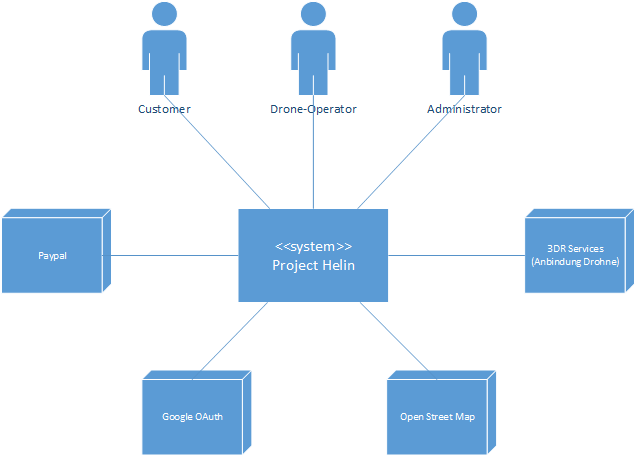
\includegraphics[width=1.0\textwidth]{images/system-context-diagram.png}
\caption{System Kontext Diagram mit externen Schnittstellen }
\label{fig:system-context-diagram}
\end{figure}










\chapter{Anforderungen}
\section{Benutzer und Personas}
Die Benutzer der Project Helin Plattform teilen sich in drei Gruppen auf:
\begin{itemize}
	\item{\textbf{Kunde:} Der Kunde möchte Produkte und Dienstleistungen nutzen, welche von Drohnen erbracht werden können. Beispielsweise die Bestellung eines Getränks und sofortige Lieferung an seine Position.}
	\item{\textbf{Administrator:} Administratoren verwenden die Project Helin Plattform, um eine Flotte von Drohnen zu verwalten. Sie nutzen dazu die Webseite der Plattform und definieren, wo ihre Drohnen fliegen dürfen und welche Produkte und Services wo angeboten werden.}
	\item{\textbf{Drone-Operator:} Der Drone-Operator ist für die Wartung der Drohne verantwortlich und verwendet dafür die Onboard-App. Er kümmert sich ausserdem um die Beladung der Drohnen.}
\end{itemize}

Bei den Personas handelt es sich um fiktive Personen.
\subsection{Persona Diego: Kunde}
\begin{minipage}{0.25\textwidth}% adapt widths of minipages to your needs
\centering
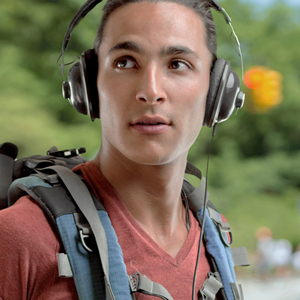
\includegraphics[width=1.0\textwidth]{images/persona-diego.jpg}
\captionof{figure}{Diego\protect\footnotemark[1]}
\label{fig:diego}
\end{minipage}%
\hfill%
\begin{minipage}{0.70\textwidth}
Diego ist \textbf{23 Jahre alt} und wohnt in einer WG in Uster.
Diego hat eine Informatik-Lehre mit BMS abgeschlossen und ist auf der Suche nach einer neuen beruflichen oder schulischen Herausforderung.
\paragraph{Technisches Verhalten}
Er arbeitet täglich acht Stunden mit dem PC und nutzt gerne neue Technologien. Er besitzt ein Android-Smartphone der neusten Generation. Die Android Updates macht er immer sofort. Interessiert sich für neue Technologien und sieht sich regelmässig Kickstarter Projekte an.
\paragraph{Ziele}
Er will sich weiterbilden und neue Herausforderungen finden. Er möchte neue Technologien entdecken und einsetzen.
\end{minipage}

\footnotetext[1]{ Freie Lizenz, \protect\url{Quelle: http://blog.placeit.net/free-avatar-pack/}}
\newpage

\subsection{Persona Stefanie: Administrator}
\begin{minipage}{0.25\textwidth}
\centering
	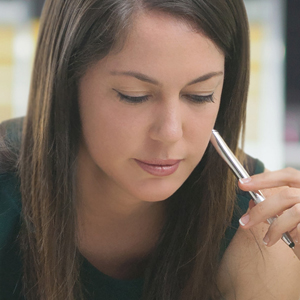
\includegraphics[width=1\textwidth]{images/persona-stefanie.jpg}
	\captionof{figure}{Stefanie \protect\footnotemark[1]}
	\label{fig:stefanie}
\end{minipage}
\hfill %
\begin{minipage}{0.70\textwidth}
Stefanie ist \textbf{33 Jahre alt} und lebt alleine in Zürich.

Als diplomierte Eventmanagerin arbeitet Stefanie bei einer Eventagentur.

\paragraph{Technisches Verhalten}
Bei der Arbeit nutzt sie vor allem Excel, Word, Outlook und Chrome als Browser. Ausserdem hat sie viel Erfahrung mit diversen mandantenfähigen Systemen (CRM, ERP), die als Web-Applikationen umgesetzt sind. Sie besitzt ein Samsung Galaxy S4, das sie schon seit einigen Jahren verwendet.
\paragraph{Kommunikationsverhalten}
Sie kommuniziert geschäftlich hauptsächlich per E-Mail. Mit Freunden unterhält sie sich oft über WhatsApp oder den Facebook-Messenger. Auch während der Arbeit verbringt sie gerne Zeit auf Facebook.
\paragraph{Ziele}
Sie möchte mit neuen und innovativen Ideen Events für Besucher spannender gestalten.
\end{minipage}

\subsection{Persona Ricardo: Drone-Operator}
\begin{minipage}{0.25\textwidth}
\centering
	
\includegraphics[width=1\textwidth]{images/persona-ricardo.jpg}
	\captionof{figure}{Ricardo \protect\footnotemark[1]}
	\label{fig:ricardo}
\end{minipage}
\hfill %
\begin{minipage}{0.70\textwidth}
Ricardo ist \textbf{26 Jahre} alt und wohnhaft in Wetzikon. Der ausgebildete Schlosser hat zurzeit keinen festen Job. Er lebt das Leben von Tag zu Tag und geniesst es, keine festen Verpflichtungen zu haben.
\paragraph{Technisches Verhalten}
Er nutzt den PC selten, vor allem aber zum Surfen im Internet. Er besitzt er ein altes Android-Smartphone. Er möchte sich auch kein neues Gerät kaufen, da er ausser WhatsApp und der Taschenlampe das Gerät nicht verwendet.
\paragraph{Kommunikationsverhalten}
Er verwendet hauptsächlich sein Mobiltelefon zur Kommunikation. Mit Freunden ist er über WhatsApp in Kontakt.
\paragraph{Ziele}
Ricardo möchte gerne mit kleinen Jobs etwas Geld dazu verdienen und ohne lange Einarbeitungszeit den Anforderungen der Eventagentur genügen.
\end{minipage}

\footnotetext[1]{ Freie Lizenz, \protect\url{Quelle: http://blog.placeit.net/free-avatar-pack/}}



\newpage


\section{Szenario}

Um eine bessere Übersicht über die Anforderungen zu erhalten wurde folgendes Szenario erstellt. Die rechtliche Situation wird dabei ausser Acht gelassen:\\

\textbf{Stefanie} hat in einem Facebook-Post von Project Helin erfahren und möchte deshalb am nächsten Openair, das ihre Firma organisiert, einen Getränke-Lieferservice mit Drohnen anbieten. Sie registriert sich und ihre Organisation auf \url{https://my.helin.ch/} und lässt sich von einem lokalen Anbieter zwei Drohnen bauen, die Getränke tragen und abwerfen können. Nach dem Aufbau des Festgeländes zeichnet sie die Flugzonen auf \url{https://my.helin.ch/} auf der Karte ein. Sie engagiert ausserdem Ricardo, der die Drohnen beladen und warten soll. Dieser lädt eine App herunter und installiert sie auf den zwei Smartphones, die auf den Drohnen montiert werden. Um die Drohnen mit dem Server zu verbinden, kann er die Adresse des Servers und einen Code eingeben, den Stefanie auf der Webseite abgeschrieben hat.\\

\textbf{Diego} möchte an einem Openair ein kühles Getränk für sich bestellen. Er hat auf einem Plakat vor Ort gesehen, dass ein Drohnen-Lieferservice existiert. Er lädt die Project Helin Bestell-App herunter und bestellt ein Rivella. Ihm wird eine Karte angezeigt mit dem voraussichtlichen Lieferort, den er bestätigen muss. Er muss sich nun einloggen und die Bestellung auf dem Mobiltelefon mit seiner Kreditkarte bezahlen.\\

\textbf{Ricardo} erhält eine Nachricht auf dem Onboard-App, die ihn fragt ob die Drohne einsatzbereit ist. Er bestätigt und ihm wird angezeigt, dass er ein Rivella laden muss. Er belädt die Drohne mit der Flasche und dem Fallschirm und bestätigt die Beladung. Die Drohne zeigt einen Countdown an und fliegt nach zehn Sekunden los. \\

\textbf{Diego} wundert sich, ob seine Bestellung unterwegs ist und sieht auf einer Karte in der App wie sich die Drohne auf ihn zubewegt. Die Drohne fliegt über ihn und wirft die Ladung ab. Danach fliegt sie auf dem gleichen Weg wieder zurück.\\

\textbf{Ricardo} sieht, dass die Drohne im Anflug ist. Sie landet an der Position, die ihm Stefanie zuvor gezeigt hatte. Er kann nun prüfen, ob die Batterie noch genug Spannung hat und ob mit der Drohne sonst alles in Ordnung ist.\\

\textbf{Stefanie} sitzt Zuhause und hat den Flug der Drohne auf \url{https://my.helin.ch/} verfolgt. Sie sieht wie sich der Stand der Batterie während des Flugs geändert hat und dass Ricardo gerade eine Drohne deaktiviert hat, bei der er die Batterie tauschen muss.

\newpage
\section{Funktionale Anforderungen (User Stories)}

Die funktionalen Anforderungen leiten sich aus der Aufgabenstellung, sowie den mit dem Betreuer diskutierten Ideen ab. Standardoperationen sind mit Teilen von \Gls{CRUD} bezeichnet. Einige Anforderungen sind mit 'zusätzlich' oder 'ausgeschlossen' gekennzeichnet, da sie nachträglich geändert wurden. Eine Erklärung zu jeder geänderten Anforderung findet sich im nächsten Abschnitt.

\subsection{Administrator}
\begin{itemize}
\item Als Administrator möchte ich auf der Webseite einen Account erstellen können.
\item Als Administrator möchte ich meine Organisation verwalten können (CRU). (zusätzlich, siehe unten)
\item Als Administrator möchte ich neue Administratoren hinzufügen und entfernen können. (zusätzlich)
\item Als Administrator möchte ich ein Projekt erfassen können.
\item Als Administrator möchte ich eine Drohne dem Projekt hinzufügen können.
\item Als Administrator möchte ich alle Drohnen verwalten können (RUD).
\item Als Administrator möchte ich Produkte verwalten können (CRUD).
\item Als Administrator möchte ich Produkte einem Projekt hinzufügen können. (zusätzlich)
\item Als Administrator möchte ich Services (z.B. Drone Selfies) verwalten können (CRUD). (optional)
\item Als Administrator möchte ich Flug-, Lade- und Abwurfzonen verwalten können (CRUD).
\item Als Administrator möchte ich Bestellungen verwalten können (CRUD). (teilweise ausgeschlossen)
\item Als Administrator möchte ich Telemetriedaten der Drohne, sowie die berechnete Route vor, nach und während der Auslieferung einer Bestellung ansehen können.
\item Als Administrator möchte ich Bestellungen abbrechen können. (ausgeschlossen)
\end{itemize}

\subsection{Kunde}
\begin{itemize}
	\item Als Kunde möchte ich eine App aus dem Google Play Store herunterladen können, um diese verwenden zu können.
	\item Als Kunde möchte ich die App nutzen, ohne mich anmelden zu müssen.
	\item Als Kunde möchte ich in der App aus einer Liste von Produkten und Services, eine Auswahl treffen können.
	\item Als Kunde möchte ich nur Produkte und Services sehen, die in meiner Umgebung angeboten werden. (zusätzlich)
	\item Als Kunde möchte ich eine Bestellung tätigen können.
	\item Als Kunde möchte ich die bestellte Ware direkt bezahlen können. (optional)
	\item Als Kunde möchte ich auf der Karte des Smartphones die Bewegung der Drohne verfolgen können um abzuschätzen wann meine Lieferung eintrifft.
	\item Als Kunde möchte ich eine Bestellung stornieren können. (ausgeschlossen)
\end{itemize}

\subsection{Drone-Operator}
\begin{itemize}
	\item Als Drone-Operator möchte ich eine Android-App mit Hilfe der heruntergeladenen \Gls{APK} installieren können.
	\item Als Drone-Operator muss ich die Drohne beim Server registrieren können.
	\item Als Drone-Operator muss ich die Drohne zu einer Organisation hinzufügen können.
	\item Als Drone-Operator muss ich das \Gls{OTG}-fähige Smartphone an einen \Gls{MAVLink} kompatiblen \Gls{Flight-Controller} über USB anschliessen können.
	\item Als Drone-Operator muss ich eine Verbindung zwischen App und Server über das Internet herstellen können.
	\item Als Drone-Operator muss ich eine Verbindung zwischen App und \Gls{Flight-Controller} herstellen können.
	\item Als Drone-Operator möchte ich den aktuellen Zustand der Verbindungen zur Drohne und zum Server sehen.
	\item Als Drone-Operator möchte ich den aktuellen Status des \Gls{Flight-Controller}s, beispielsweise GPS und Batteriespannung, sehen.
	\item Als Drone-Operator möchte ich eine Liste von Produkten angezeigt bekommen, die für die aktuelle Mission geladen werden müssen.
	\item Als Drone-Operator möchte ich eine Mission annehmen oder ablehnen können, um eine Drohne bei Problemen austauschen zu können.
	\item Als Drone-Operator möchte ich die Beladung einer Drohne bestätigen können.
	\item Als Drone-Operator erhalte ich ein visuelles und akustisches Countdown-Signal bevor die Drohne startet.
	\item Als Drone-Operator möchte ich den Start der Drohne während des Countdowns verhindern können.
\end{itemize}

\subsection{Nachträglich ausgeschlossene Anforderungen}

\subsubsection{Bestellung löschen und ändern}
Gemäss den anfänglichen Anforderungen sollte der Administrator die Möglichkeit haben eine Bestellung zu bearbeiten (\Gls{CRUD}). Dies wurde reduziert auf das Ansehen von Bestellungen (R). Unserer Meinung nach, sollte nur der Kunde die Möglichkeit haben seine Bestellung zu löschen. Ausserdem muss es auch dort Einschränkungen geben, da eine bezahlte Bestellung unter keinen Umständen gelöscht werden darf.

\subsubsection{Mission abbrechen}

Das Abbrechen einer Mission wurde aus dem Scope entfernt, da sich einerseits Fragen über den sinnvollen Einsatz eines solchen Features stellten und andererseits wichtigere Tasks wie die Bezahlung im App priorisiert werden konnten.

\subsection{Nachträglich hinzugefügte Anforderungen}

\subsubsection{Verwalten von Organisationen}

Um die Applikation mandantenfähig zu machen, wurden Organisationen eingefügt. Diese trennen verschiedene Kunden komplett ab und ermöglichen den Einsatz als Software as a Service.

\subsubsection{Administratoren hinzufügen und entfernen}

Um Organisationen nutzbar zu machen, muss es auch möglich sein, zusätzliche Administratoren zu einer Firma hinzuzufügen und wieder zu entfernen.

\subsubsection{Produkte einem Projekt hinzufügen}

Dieses Feature war nötig, damit Organisationen ihre Produkte nur einmal erfassen müssen und diese dann für verschiedene Projekte (z.B. Events) verwendet werden können (siehe Abb. \ref{fig:domain-model}).

\subsubsection{Nur verfügbare Produkte anzeigen}

Es macht keinen Sinn, dass ein Kunde Produkte sieht, die gar nicht zu ihm geliefert werden können. Deshalb wird die Liste mit Hilfe seiner Position auf verfügbare Produkte gefiltert.

\newpage
\section{Nichtfunktionale Anforderungen}

\subsection{Android Kompatibilität}
\begin{tabular}{|p{.25\textwidth}|p{.75\textwidth}|} \hline
	Synopsis & Die Onboard-App funktioniert mit Android 4.4 und die Customer-App mit Android 6.1\\ \hline
	Messbarkeit & Die obengenannten Apps können alle funktionalen Anforderungen erfüllen, wenn sie mit Android 4.4 bzw. 6.1 gestartet werden.\\ \hline
\end{tabular}

\subsection{Verbindungsabbruch}
\begin{tabular}{|p{.25\textwidth}|p{.75\textwidth}|} \hline
	Synopsis & Verbindungsabbruch der Onboard App zum Server soll keine negativen Auswirkungen auf die Mission haben.  \\ \hline
		
	Messbarkeit & Nach dem Start der Mission schliesst die Drohne, auch ohne Verbindung zum Server, die Mission ab. \\ \hline
\end{tabular}

\subsection{Flugsicherheit}
\begin{tabular}{|p{.25\textwidth}|p{.75\textwidth}|} \hline
	Synopsis & Eine Drohne führt vor dem Freigeben der Motoren (Arming) einen Check durch, der prüft ob alle nötigen Voraussetzungen für einen Start erfüllt sind. Ausserdem müssen vor einem Start ebenfalls Voraussetzungen der Mission erfüllt sein, beispielsweise muss der Drone-Operator den Start freigeben. Sollte eine dieser Vorraussetzungen nicht erfüllt sein, darf die Drohne nicht starten.  \\ \hline
	
	Messbarkeit & Drohne startet nicht, falls der Pre-Flight-Check des Autopiloten nicht erfolgreich war oder Voraussetzungen für die aktuelle Mission nicht erfüllt sind. \\ \hline
\end{tabular}
\subsection{Verbindungswiederherstellung}
\begin{tabular}{|p{.25\textwidth}|p{.75\textwidth}|} \hline
	Synopsis & Nach einem Verbindungsabbruch zwischen dem Server und der Onboard App soll die Verbindung wiederhergestellt werden sobald wieder eine Internetverbindung verfügbar ist. \\ \hline
	
	Messbarkeit & Die Verbindung zwischen Server und App wird nach dem deaktivieren und wieder aktivieren der Internetverbindung(4G) innert 30 Sekunden wiederhergestellt.\\ \hline
\end{tabular}

\subsection{Security}
\subsubsection{Sichere Messaging-Verbindungen}
\label{sec:message-security}
\begin{tabular}{|p{.25\textwidth}|p{.75\textwidth}|} \hline
	Synopsis & Es darf nicht möglich sein, dass jemand die Steuerung einer beim Server registrierten Drohne übernehmen kann.\\ \hline
	Messbarkeit & Der Übertragungskanal vom Server zur Drohne ist verschlüsselt, sodass sich keine weiteren \Gls{Message-Producer} anmelden können.\\ \hline
\end{tabular}

\subsubsection{Sichere HTTP-Verbindungen}
\begin{tabular}{|p{.25\textwidth}|p{.75\textwidth}|} \hline
	Synopsis & Neben der Messaging Verbindung muss auch die HTTP-Verbindung gesichert sein.\\ \hline
	Messbarkeit & Die Verbindung über den Webbrowser lässt nur HTTPS zu. Die Verbindung vom Customer-App zum Server läuft über HTTPS und Secure-WebSockets. Die Verbindung vom Onboard-App zum Server läuft über HTTPS.\\ \hline
\end{tabular}

\section{Usability und Accessability}

Usability-Tests und Anforderungen in der Accessability wurden bewusst und in Absprache mit dem Betreuer aus dem Scope ausgeschlossen.

\section{Domain-Model}
Aus den funktionalen Anforderungen ergibt sich das folgende Domainmodel.
\begin{landscape}
\begin{figure}[h]
	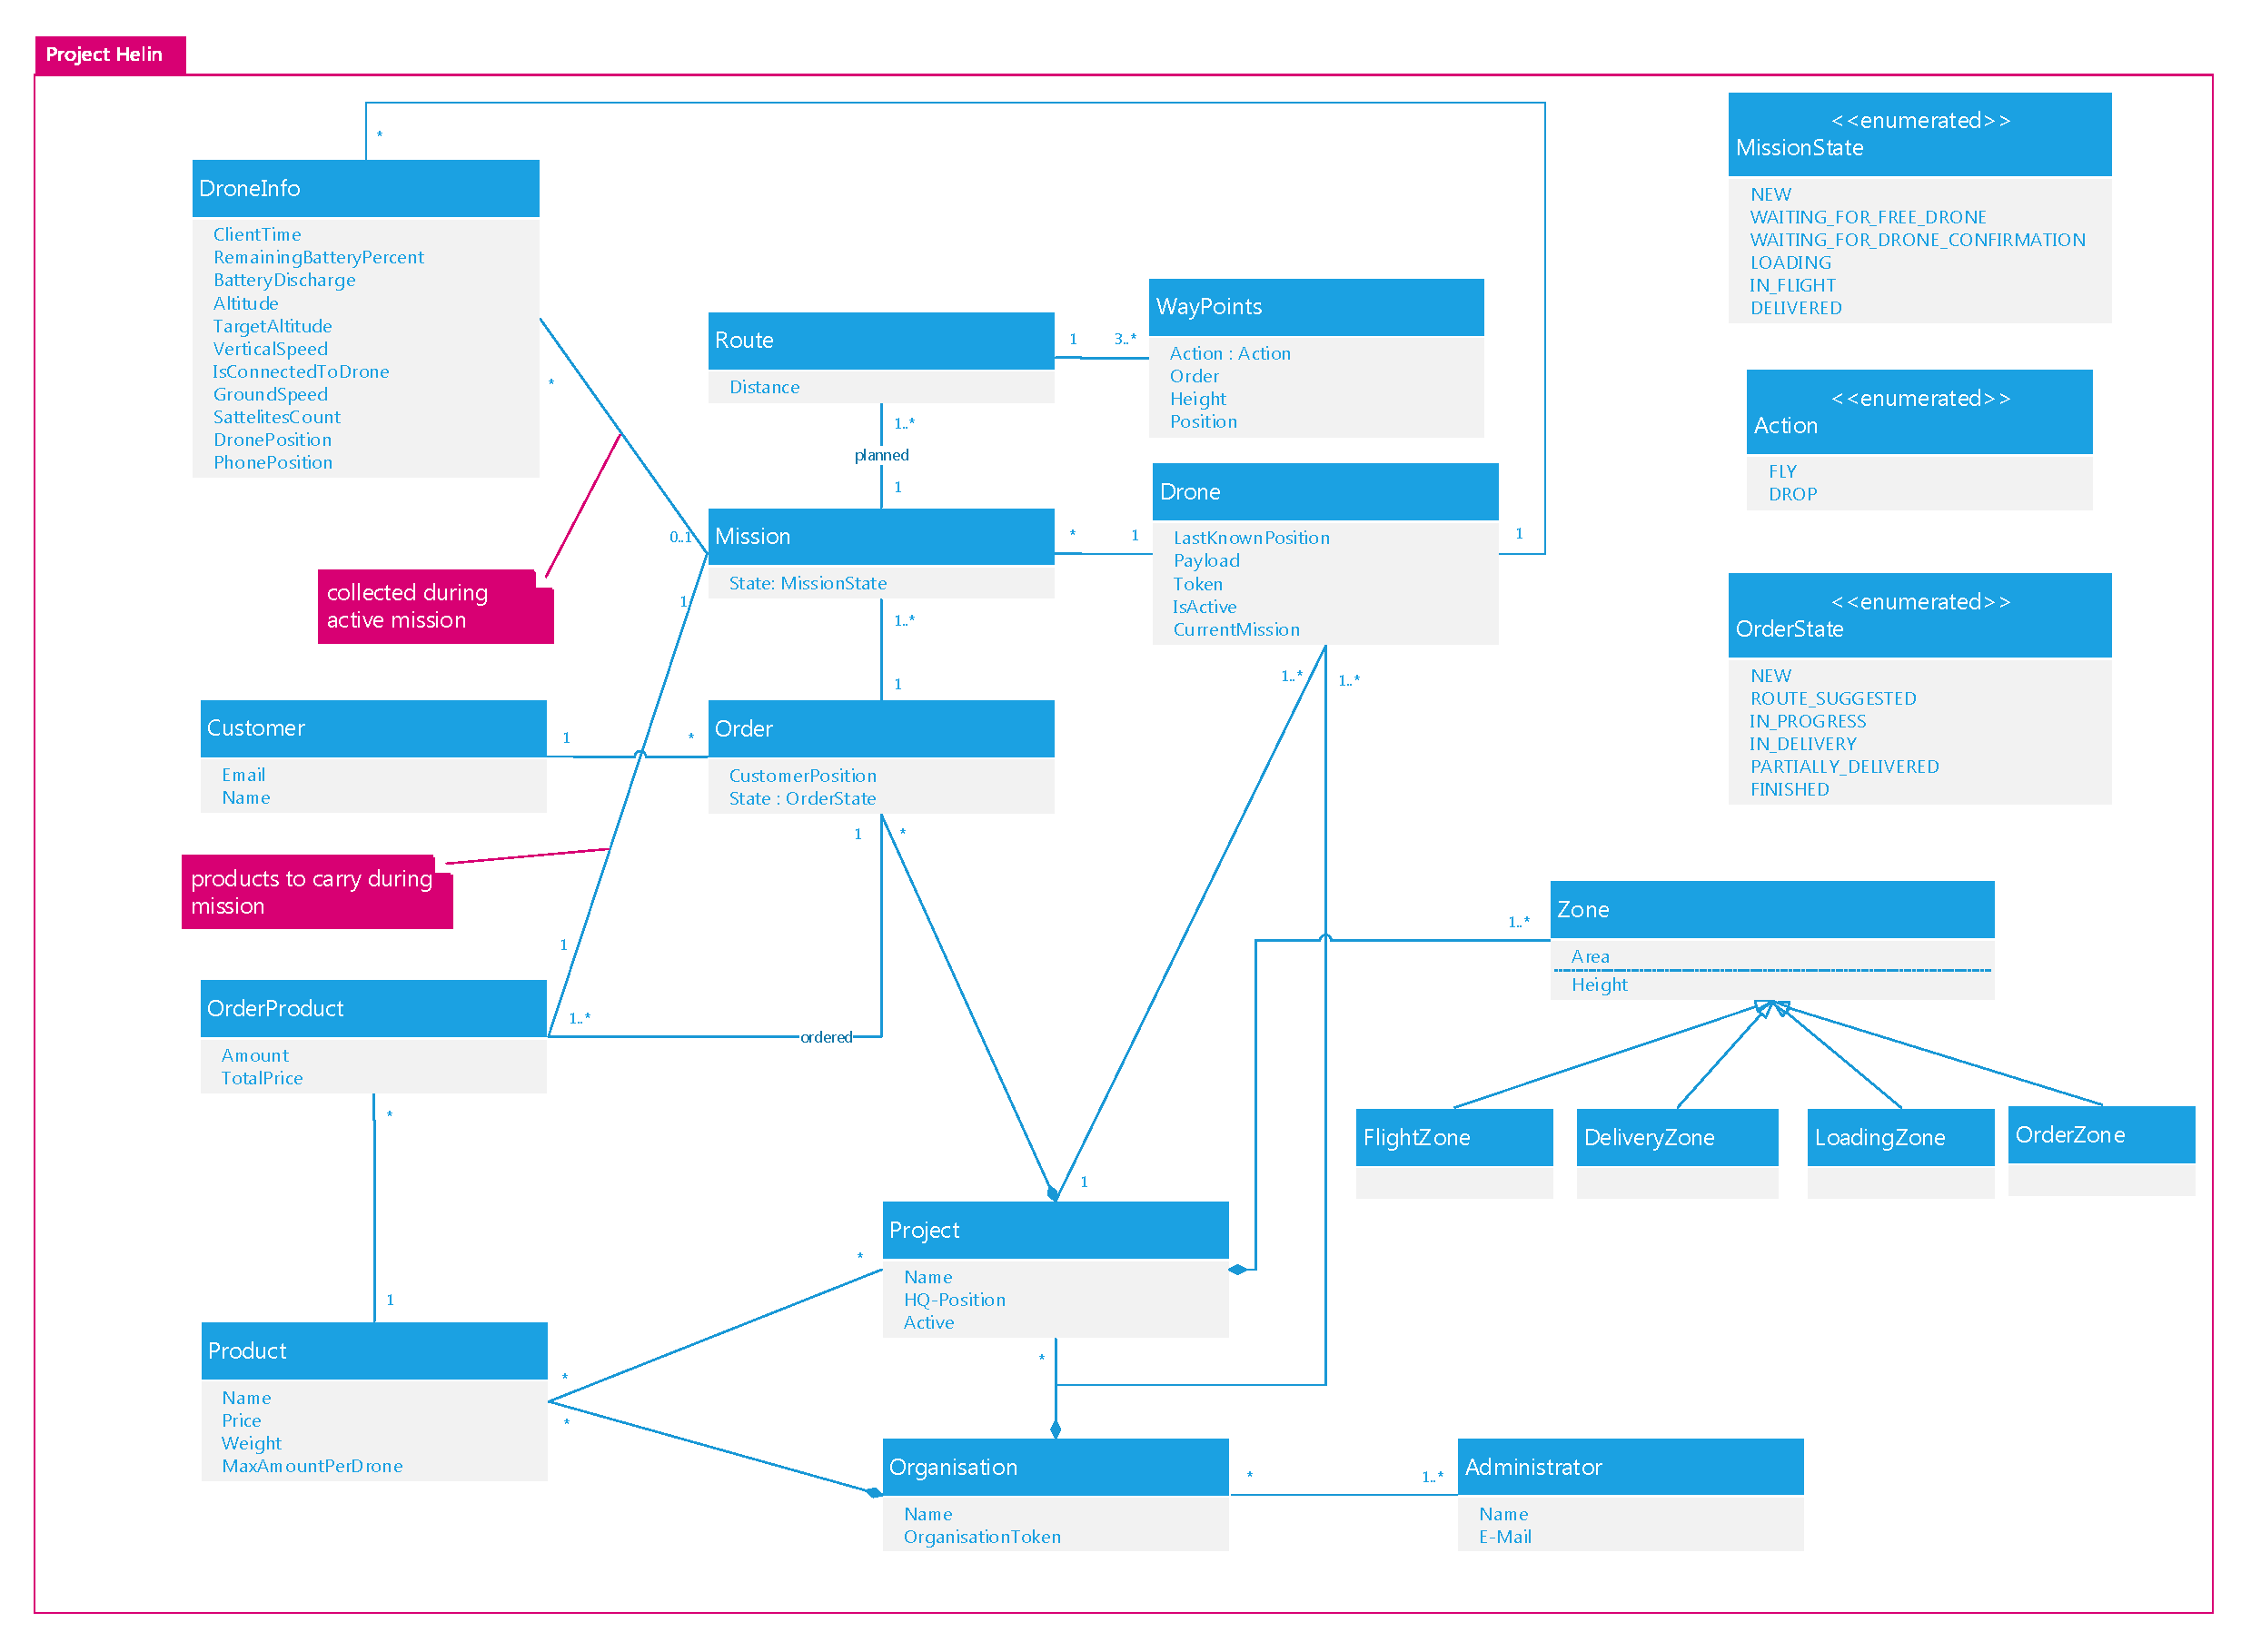
\includegraphics[width=0.75\paperheight]{images/domainmodell.pdf}
	\caption{Domain-Model}
	\label{fig:domain-model}
\end{figure}
\end{landscape}


\chapter{Architektur}

\section{Ziele}

Die folgende Architektur soll es ermöglichen, eine Flotte von Drohnen automatisiert und zentralisiert zu verwalten. Die Kommunikation zwischen Server und Drohne muss ausserdem von beiden Seiten initiierbar sein (Push-Messages). Zusätzlich muss eine Schnittstelle für Kunden existieren, damit Bestellungen getätigt werden können. 


\section{Einschränkungen}

Da der Flight-Controller bereits vor Anfang der Arbeit bestellt wurde, wird dieser als vorgegebene Limitierung angesehen. Somit steht auch die Wahl auf MAVLink, für die Kommunikation mit der Drohne fest.  


\section{Übersicht}

Die Abbildung \ref{fig:architecture-overview} zeigt eine Übersicht der verschiedenen Tiers und Server-Komponenten.

\begin{figure}[H]
	\centering
	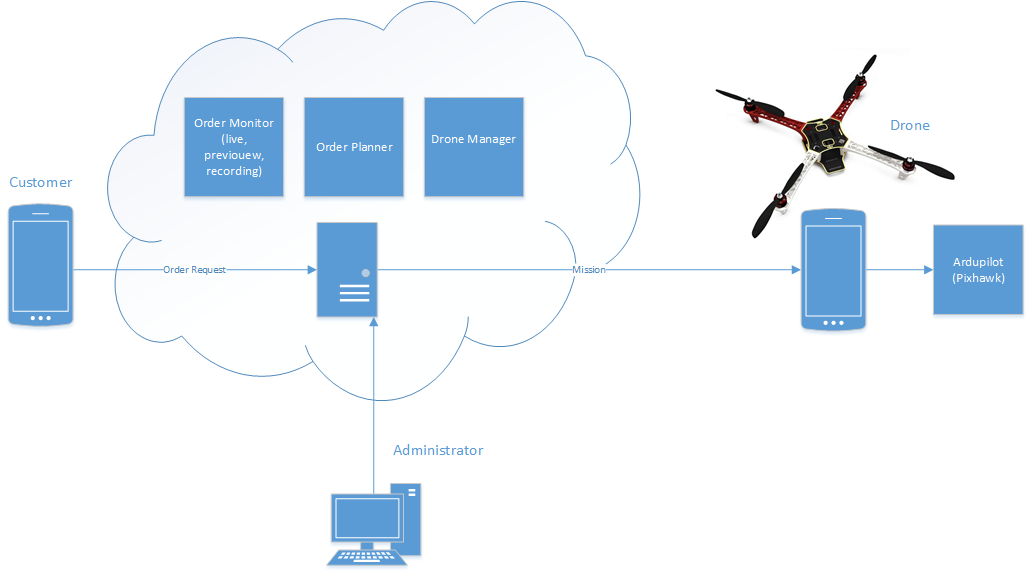
\includegraphics[width=0.8\textwidth]{images/Overview-Diagram.png}
	\caption{Übersicht der Project Helin Architektur }
	\label{fig:architecture-overview}
\end{figure}

\section{Logische Architektur}

\subsection{Komponenten Übersicht}

Abbildung \ref{fig:logical-architecture-overview} zeigt die Hauptkomponenten, sowie eine Übersicht der enthaltenen Layer und Packages. Ausserdem sind die Abhängigkeiten zu den wichtigsten externen Komponenten dargestellt. Hervorzuheben ist ebenfalls die gemeinsame Verwendung der Commons-Komponente. 

\begin{figure}[H]
	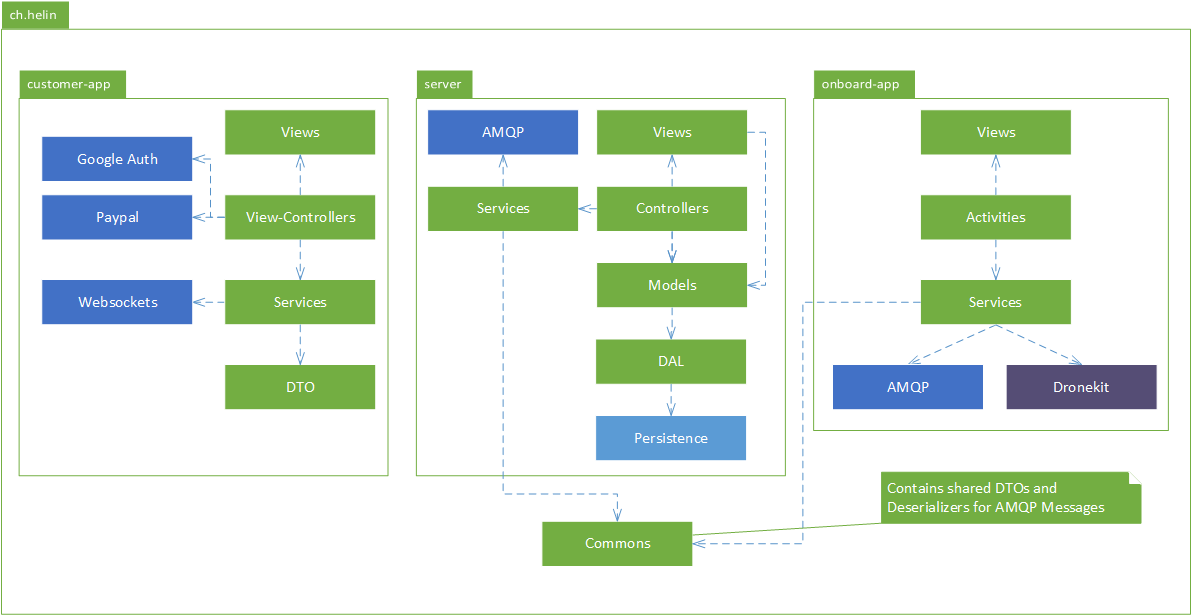
\includegraphics[width=1.0\textwidth]{images/logical-architecture-overview.png}
	\caption{Vereinfachte Übersicht der logischen Architektur und deren Komponenten }
	\label{fig:logical-architecture-overview}
\end{figure}

\section{Server-Komponente}

\subsection{Anforderungen}
Aus den in den Anforderungen definierten Zielen, ergeben sich für die Server-Komponente folgende Anforderungen:

\begin{itemize}
	\item Bietet Benutzeroberfläche für Administratoren
	\item Verwaltet CRUD für alle nötigen Klassen (siehe Domain Model)
	\item Verwaltet Verbindungen zu Onboard-Apps und Customer-Apps
	\item Berechnet Flugrouten basierend auf den erhaltenen Bestellungs-Koordinaten
\end{itemize}

\subsection{Layers}
Die Architektur des Servers basiert auf dem {MVC Pattern \cite{MVC}}, da dieses für CRUD Applikationen mit Benutzeroberfläche besonders geeignet ist und dafür viele geeignete Frameworks zur Verfügung stehen.\\

Für Komponenten die aus unterschiedlichen Controllern verwendet werden, wurde zusätzlich eine Service Komponente verwendet. Die Services stellen Abstraktionen für wichtige Funktionen wie das Messaging und die Routenberechnung bereit.\\

Die Verantwortlichkeiten und Kollaborationen der Layer werden nachfolgend genauer definiert.

\subsubsection{View-Layer}
Stellt die grafische Benutzeroberfläche zur Verfügung und rendert diese basierend auf den Model-Daten.

\subsubsection{Controller-Layer}
\begin{tabular}{|p{.70\textwidth}|p{.30\textwidth}|} \hline
	\textbf{Verantwortlichkeiten} & \textbf{Zusammenarbeit} \\ \hline \hline
	\begin{itemize}
		\item Lädt Daten für Views aus dem Data-Access-Layer
		\item Verarbeitet eingehende HTTP-Requests
		\item Verarbeitet eingehende Messages aus den Messaging-Queues
		\item Enthält Business-Logik und steuert Ablauf nach einem Request	
	\end{itemize}&
	\begin{itemize}
		\item Data-Access-Layer
		\item Service-Layer
		\item Model-Layer
		\item Messages
	\end{itemize}
	\\ \hline
\end{tabular}

\subsubsection{Model-Layer}

Der Model-Layer enthält die Datenmodelle. (siehe Domain Model)

\subsubsection{Service-Komponente}

\begin{tabular}{|p{.70\textwidth}|p{.30\textwidth}|} \hline
	\textbf{Verantwortlichkeiten} & \textbf{Zusammenarbeit} \\ \hline \hline
	
	\begin{itemize}
		\item Verwaltet Verbindungen zu den Drohnen
		\item Deserialisiert eingehende Nachrichten
		\item Leitet eingehende Nachrichten von Drohnen an den Controller-Layer weiter	
		\item Leitet eingehende Nachrichten von Customers an den Controller-Layer weiter	
		\item Berechnet Flugrouten basierend auf den vorgegebenen Flugzonen
	\end{itemize}&
	\begin{itemize}
		\item Controller-Layer
		\item AMQP-Library
		\item Messages
	\end{itemize}
	\\ \hline
\end{tabular}

\subsubsection{Data-Access-Layer (DAL)}

Der Data Access Layer bietet die Möglichkeit auf die Persistence Library zuzugreifen und stellt dafür die wichtigsten Funktionen zur Verfügung. 

\section{Onboard-App}

\subsection{Anforderungen}

\begin{itemize}
	\item Kommuniziert mit dem Flight-Controller der Drohne
	\item Kommuniziert mit dem Server
	\item Bietet eine Benutzeroberfläche für den Drone-Operator 
\end{itemize}

\subsection{Layer}

Die App enthält die normalen Android-Application-Layer wie Activities und Views. Zusätzlich kommt der Service-Layer hinzu. Dieser enthält keine Android-Services, sondern selbst entwickelte Service-Klassen. Android Services werden nur zwingend benötigt, wenn etwas im Hintergrund weiterlaufen soll. Da die Onboard-App aber immer im Vordergrund läuft, konnte die aufwendige Kommunikation mit Android-Services mit Hilfe von {Dependency-Injection \cite{DI} umgangen werden.\\

\subsubsection{Service-Komponente}

\begin{tabular}{|p{.70\textwidth}|p{.30\textwidth}|} \hline
	\textbf{Verantwortlichkeiten} & \textbf{Zusammenarbeit} \\ \hline \hline
	
	\begin{itemize}
		\item Verwaltet Verbindung zur Drohne
		\item Verwaltet Verbindung zum Server
		\item Deserialisiert eingehende Nachrichten.
		\item Leitet eingehende Nachrichten vom Server and den Activities-Layer oder andere Services weiter
		\item Ermöglicht das Senden von Nachrichten an den Server
	\end{itemize}&
	\begin{itemize}
		\item Activities-Layer
		\item AMQP-Library
		\item Commons
	\end{itemize}
	\\ \hline
\end{tabular}


\section{Customer-App}

\subsection{Anforderungen}

\begin{itemize}
	\item Kommuniziert mit dem Server
	\item Bietet eine Benutzeroberfläche für den Customer
	\item Ermöglicht die Bezahlung von Produkten
	\item Ermöglicht das Login über einen externen Identifikationsprovider
\end{itemize}

\subsection{Layer}

\subsubsection{View-Layer}
Ist zuständig für die Darstellung der Benutzeroberfläche und bindet die Schnittstellen zum Zahlungsanbieter und Identifikationsprovider an.

\subsubsection{Service-Layer}
\begin{tabular}{|p{.70\textwidth}|p{.30\textwidth}|} \hline
	\textbf{Verantwortlichkeiten} & \textbf{Zusammenarbeit} \\ \hline \hline
	
	\begin{itemize}
		\item Verwaltet Verbindung zum Server
		\item Deserialisiert eingehende Nachrichten.
		\item Leitet eingehende Nachrichten vom Server and den Activities-Layer weiter
		\item Ermöglicht das Senden von Nachrichten an den Server
	\end{itemize}&
	\begin{itemize}
		\item View-Layer
		\item WebSockets-Library
		\item Identifikationsprovider
		\item Zahlungsanbieter
	\end{itemize}
	\\ \hline
\end{tabular}

\section{Kommunikations-Architektur}
\label{sec:communication-architecture}
Die Abbildung \ref{fig:communication-architecture-overview} zeigt die Kommunikations-Architektur in der Übersicht. Wichtig sind vor allem die verschiedenen verwendeten Protokolle, die benötigt werden um die Anforderungen erfüllen zu können. Für die Kommunikation mit dem Onboard-App wird Messaging ({\Gls{AMQP}) verwendet, um bidirektionale Kommunikation zu ermöglichen und die höchstmögliche Zuverlässigkeit zu erreichen. Eine bidirektionale bzw. beidseitig initiierbare Kommunikation ist bei allen Geräten nötig um Live-Updates zu ermöglichen (Verfolgung der Drohne). Ausserdem muss die eingesetzte Technologie für die Kommunikation zwischen dem Server und den Onboard-App den Nicht-Funktionalen-Anforderungen gerecht werden, die im Bezug auf Verbindungsabbrüche und Verbindungswiederherstellung bestehen.\\
	
Bei der Anbindung der Customer-App steht die Platzformunabhängigkeit der Schnittstelle mehr im Vordergrund als die Zuverlässigkeit der bidirektionalen Verbindung. Einzig die Liveupdates der Drohnenposition werden über diese Verbindung gesendet. Deswegen wird dort vor allem HTTP verwendet und nur wo nötig WebSockets eingesetzt. Damit können in Zukunft auch andere Geräte verwendet werden um das System anzusprechen, ohne dass sie ein Messaging-Protokoll unterstützen müssen.\\

Die Anbindung an die Administrationsoberfläche erfolgt ebenfalls über HTTP und WebSockets, da dort die Wahrscheinlichkeit eines Verbindungsabbruchs viel geringer ist als bei einem mobilen Gerät.\\

\begin{figure}[H]
	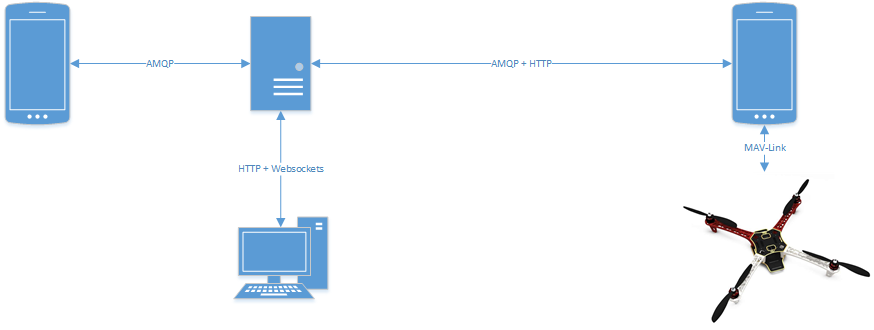
\includegraphics[width=1.0\textwidth]{images/Communication-Overview-Diagram.png}
	\caption{Übersicht der Kommunikations-Architektur mit den jeweiligen Protokollen. }
	\label{fig:communication-architecture-overview}
\end{figure}

\subsection{Verwendete Enterprise Integration Patterns}
Messaging-Systeme und Protokolle bieten eine grosse Auswahl an Patterns die je nach Anforderungen verwendet werden können.({\cite{EIP}}) Für dieses Projekt benötigen wir nur einen kleinen Teil davon um den gestellten Anforderungen gerecht zu werden.
%
\subsubsection{Point-to-Point Channel}
Um zwischen einer registrierten Drohne und dem Server einen sicheren und zuverlässigen Nachrichtenaustausch zu ermöglichen, wird jede Drohne bzw. jede App über einen separaten Point-to-Point Channel	\cite[S. 103]{EIP}} angebunden. Der Channel wird nach der Registrierung zugeteilt und stellt den Point-to-Point Kanal zwischen Drohne und Server dar. Dies garantiert dem Server, eine Nachricht an nur eine Drohne zu schicken.
%
\subsubsection{At-most-once}

Die Fehlersemantik At-most-once gibt die Sicherheit, dass eine Drohne eine Mission oder einen Befehl nur ein Mal erhält. Ansonsten müsste das System idempotent gebaut werden. Exactly-once delivery ist ausserdem in der Praxis eigentlich unmöglich umzusetzen, weshalb wir uns für diese Alternative entschieden haben. 
%
\subsubsection{Event-driven Consumer}
{Event-driven Consumer \cite[S. 442]{EIP}} Systeme bieten die Möglichkeit auf Grund von Nachrichten Aktionen auszuführen. Beispielsweise:
%
\begin{itemize}
	\item Drohne erhält neue Mission vom Server und soll dies dem Drone-Operator anzeigen.
	\item Server erhält neue Position von der Drohne und soll diese Nachricht dem Kunden weiterleiten und dem Administrator auf dem Web-Client anzeigen.
	\item Smartphone des Kunden erhält neue Position der Drohne, auf der Karte wird die Position der Drohne angezeigt.
\end{itemize}

\section{Bestellprozess}

Order Cargo (Abbildung \ref{fig:registerDrone}) beschreibt den Bestellprozess und die damit zusammenhängende Kommunikation. \\

Der Kunde bestellt mittels der App ein Produkt, der Server bestätigt ihm die Bestellung und schlägt einen Abwurfort vor. Sollte der Abwurfort dem Kunden nicht entsprechen, so kann er den Prozess abbrechen und ihn noch einmal auslösen, sobald er sich an einer passenderen Stelle befindet.\\

Der Server analysiert die Eignung der verfügbaren Drohnen und bestimmt im Anschluss eine, welche den Auftrag ausführen kann und zeigt die Mission dem Drone-Operator an. Sollte die Drohne bereit sein, so kann er diesen Auftrag bestätigen. Im Falle einer nötigen Wartungsarbeit kann der Auftrag zu diesem Zeitpunkt auch abgelehnt werden. Sobald der Auftrag angenommen wurde, erhält der Drone-Operator genaue Angaben zur Beladung der Drohne. Anschliessend wird die Ladung bestätigt und der Server kann dem Kunden mitteilen, dass die Drone startklar ist. Während des Fluges erhält der Kunde Benachrichtigungen vom Server mit der aktuellen Position der Drohne. Sobald die Ladung abgeworfen wurde, fliegt die Drohne zur Ladezone zurück und bestätigt dem Server die Ankunft. So kann gewährleistet werden, dass bekannt ist, ab wann die Drohne wieder verfügbar ist. \\

Der Bezahl- und Anmeldeprozess wird hier aus Übersichtsgründen nicht dargestellt.
\begin{figure}[H]
	\centering
	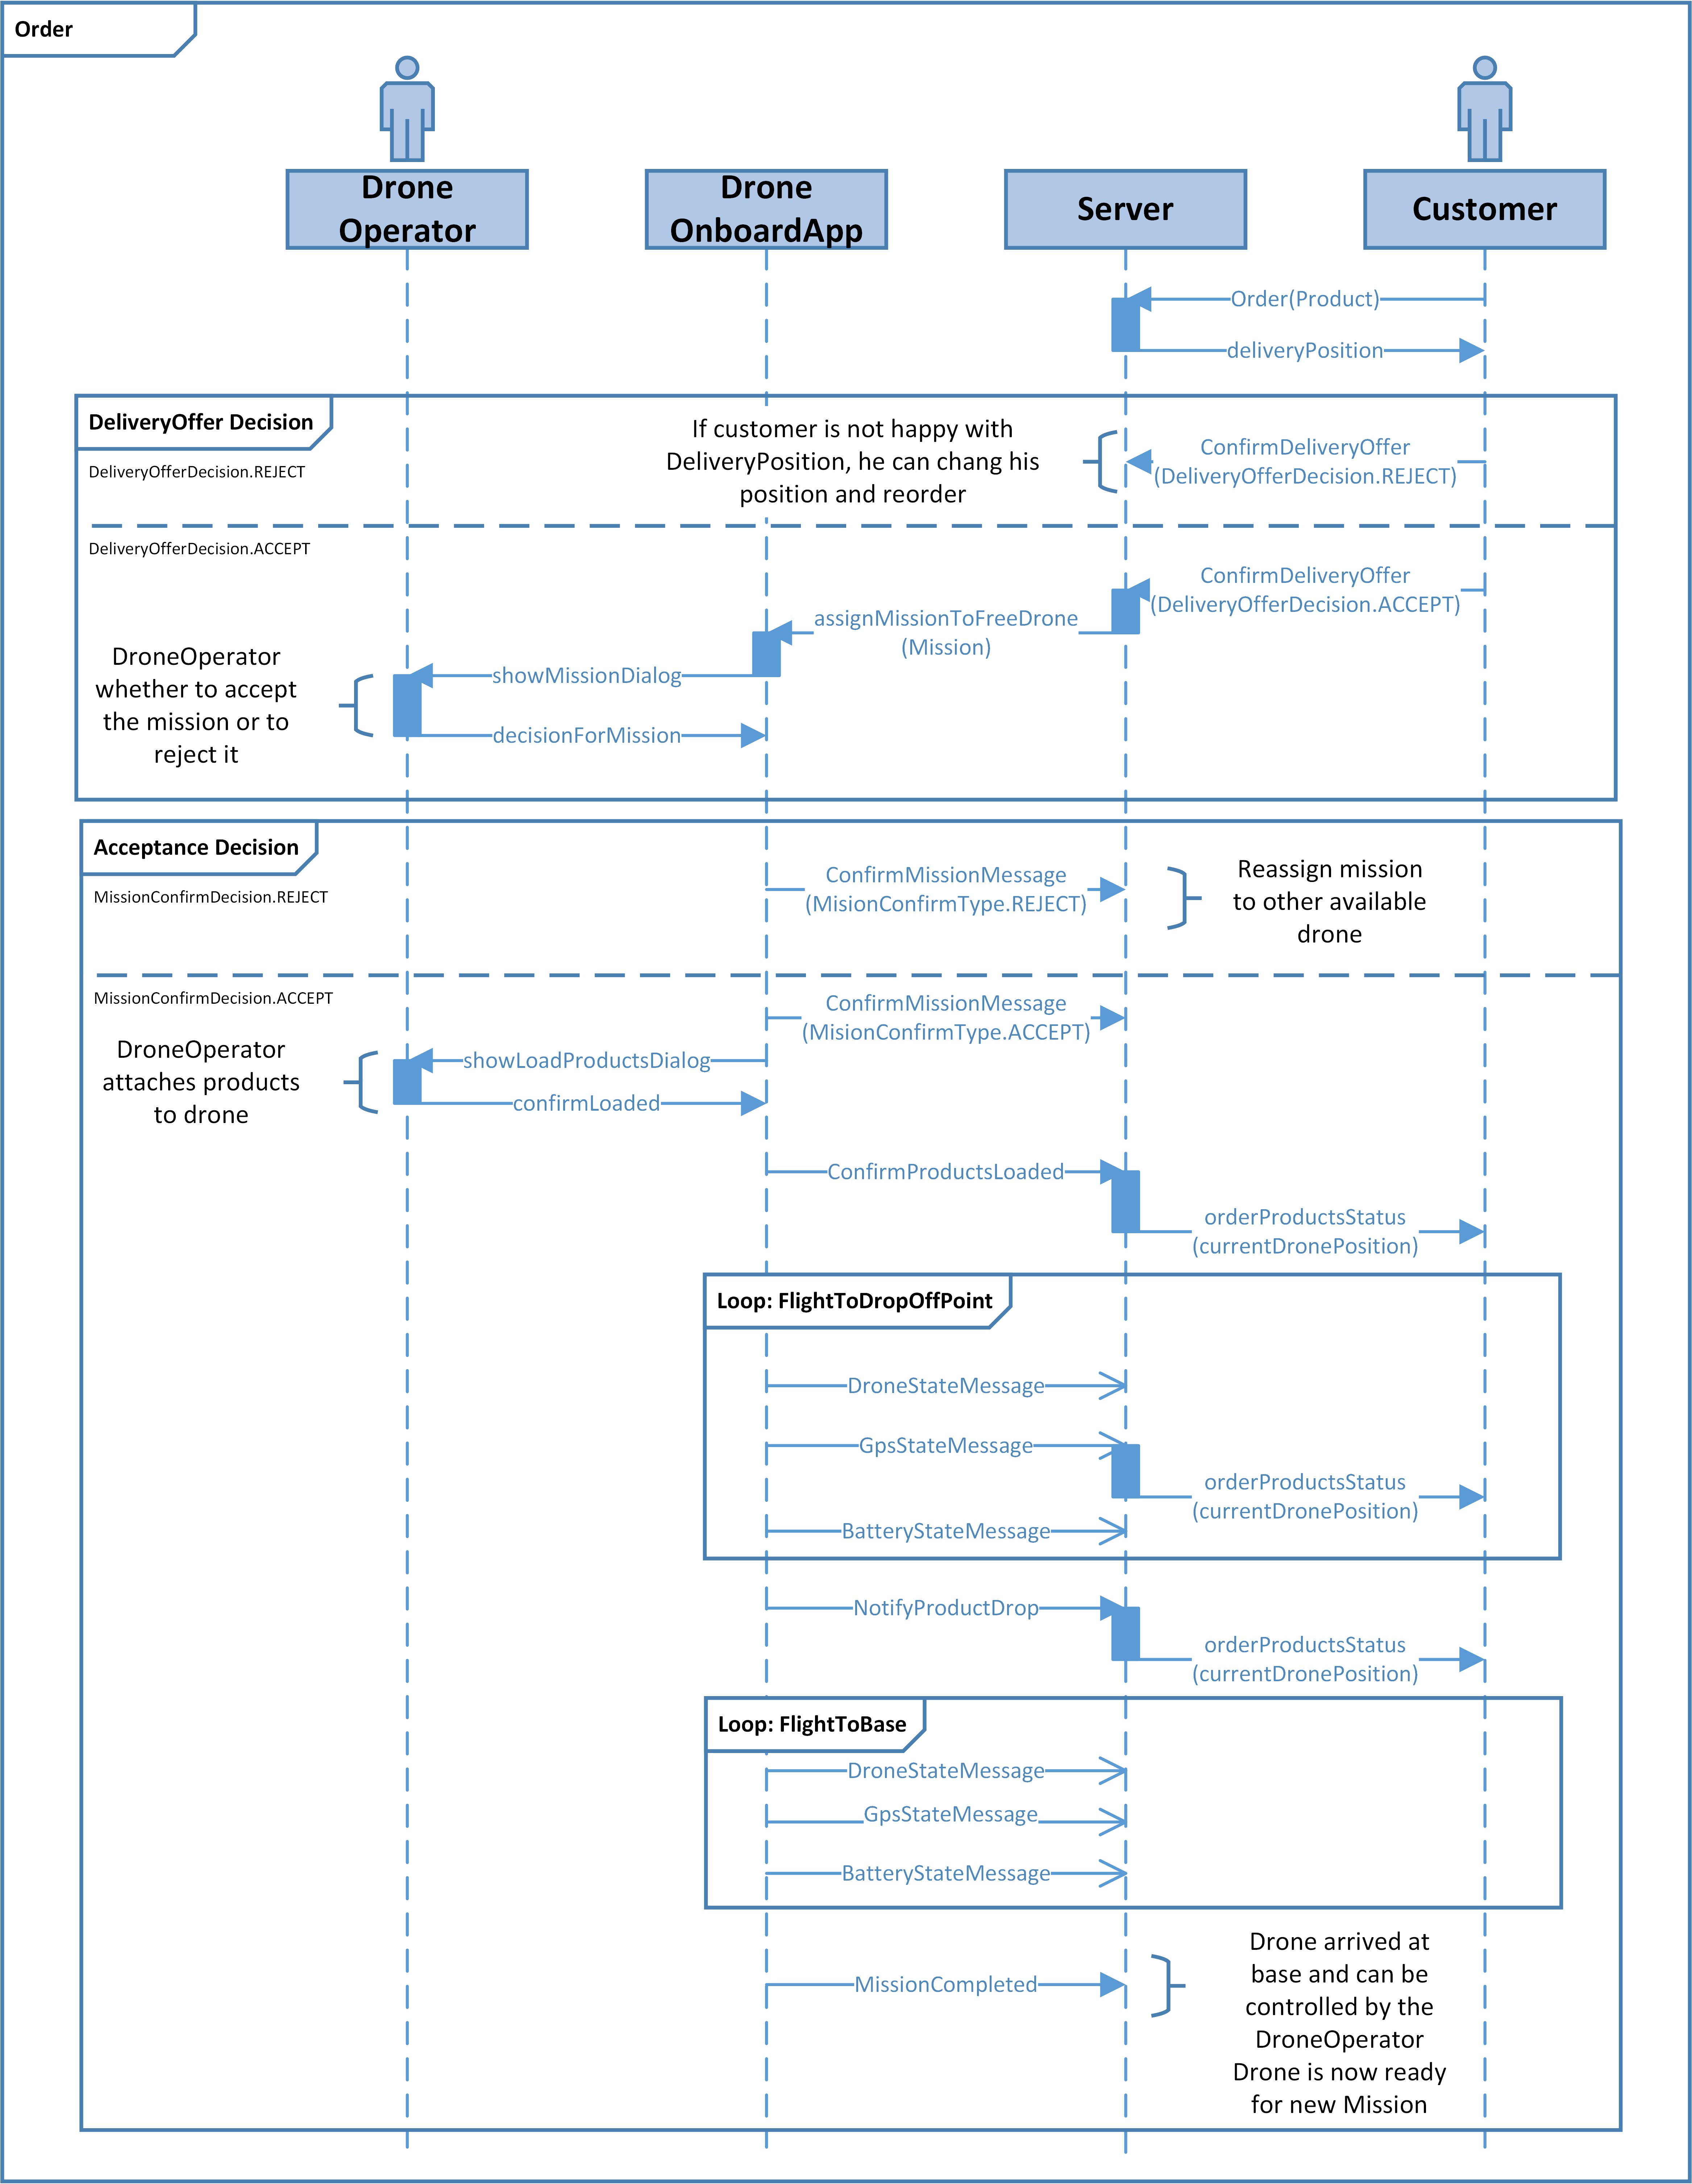
\includegraphics[height=1.0\textheight]{images/sequence_diagram.png}
	\caption{Übersicht der Project Helin Architektur }
	\label{fig:registerDrone}
\end{figure}

\section{Missionen}

Wie im Domainmodel (Abb. \ref{fig:domain-model}) ersichtlich, enthalten alle Bestellungen mindestens eine Mission. Die Mission wiederum enthält alle Informationen, die für die Auslieferung notwendig sind. Das folgende Diagramm (Abb. \ref{fig:mission-state}) zeigt die möglichen Zustände einer Mission, von der Bestellung bis zur Rückkehr nach der Lieferung.

\begin{figure}[h]
	\centering
	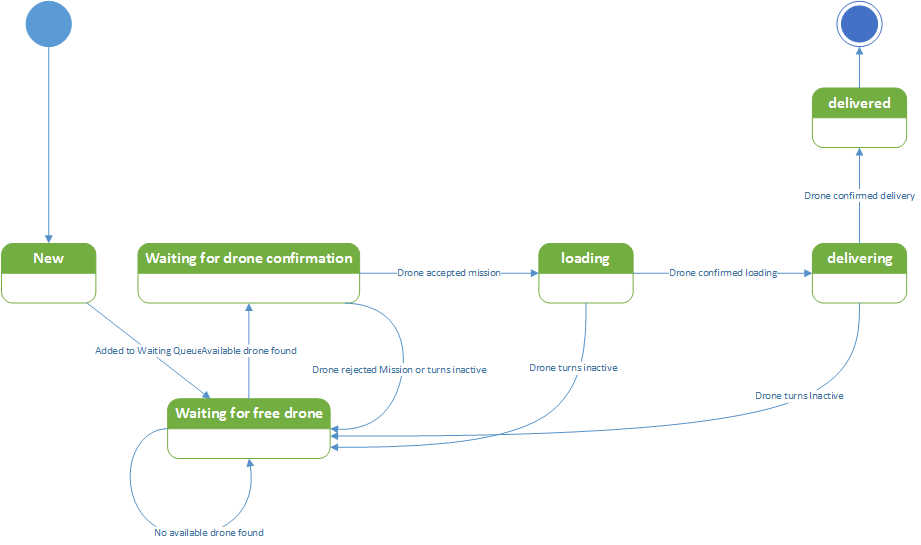
\includegraphics[width=1.0\textwidth]{images/mission-state-flow-diagram.png}
	\caption{Zustände der Mission}
	\label{fig:mission-state}
\end{figure}
\newpage
\chapter{Umsetzung}

\section{Implementierung}

\subsection{Server}

\subsubsection{Verwendete Bibliotheken}
\begin{tabularx}{\textwidth}{|X|X|c|X|}
	\hline
	\textbf{Name} & \textbf{Verwendungszweck} & \textbf{Version} & \textbf{Lizenz} \\
	\hline \hline
	Hibernate ORM Mapper & Objekt-Relationales mapping zwischen Datenbank und Models  & 5.1.0 & Apache 2.0\\
	\hline 
	RabbitMQ Client & Client Komponente zur Kommunikation mit dem Rabbit MQ Server & 3.6.0 &  Mozilla Public License 1.1, GPL 2, Apache 2.0 \\
	\hline 
	jGraphT & Graph Bibliothek für Java, um effizient Operationen auf dem Graph auszuführen & 0.9.2 &  LGPL, EPL \\
	\hline 
	\hline
	\textbf{Name} & \textbf{Verwendungszweck} & \textbf{Version} & \textbf{Lizenz} \\
	\hline \hline
	Google GSON & Java Serialisierungs / Deserialisierungs Bibliothek & 2.6.2 & Apache 2.0\\
	\hline 
\end{tabularx}

\subsection{Onboard-App}

\subsubsection{Verwendete Bibliotheken}
\begin{tabularx}{\textwidth}{|X|X|c|X|}
	\hline
	\textbf{Name} & \textbf{Verwendungszweck} & \textbf{Version} & \textbf{Lizenz} \\
	\hline \hline
	DroneKit-Android Client & Android API für MAV-Link Protokoll zum ansteuern der Drohne & 1.5.1 & Apache 2.0\\
	\hline 
	AMQP Messaging Library & Messaging für Android & 3.6.0 &  Mozilla Public License 1.1, GPL 2,  Apache 2.0 \\
	\hline 
	Lyra  & High availability Messaging & 0.4.3 &  Apache 2.0 \\
	\hline 
\end{tabularx}
\subsection{Customer App}
Gemäss Aufgabenstellung sollte ein Prototyp für eine App, mit welchem Bestellungen am System abgegeben können, entwickelt werden.
Diese App wurde als letzte Komponente entwickelt, da sie erst getestet werden konnte als die Server- und Onboard-App-Komponenten fertiggestellt waren.

Um manuelle Tests der Bestell-API möglich zu machen, wurde in der Administrations-Seite eine "'Fake Order"' Funktionen eingeführt. 
Diese imitiert eine Bestellung des Kunden und schickt eine Anfrage mit vordefinierten Koordinaten und Produkten an das System.

\begin{figure}[H]
	\centering
	
\includegraphics[width=1\textwidth] {images/customer-app-fake-order.png}
	\caption{Send Fake Order within Administrator Page}
\end{figure}

Anders als die Onboard-App, welche native mit Java entwickelt wurde und nur auf Android läuft, entschieden wir uns beim Bestell-App für eine Cross-Plattform Lösung, welche Android und iOS unterstützt. 

Auch wenn gemäss der Aufgabenstellung keine iOS App gefordert war, stelle sich doch die Frage ob man die iPhone-Kunden ausschliessen soll und spätere Entwickler zwingt, einen grossen Teil des Codes in einer nativen iOS App duplizieren zu müssen. Mit einem Marktanteil von 42.2\% (Zahlen 2015) \cite{ios-user} von iOS Benutzern in der Schweiz, ist anzunehmen, dass zu einem späteren Zeitpunkt eine iPhone App implementiert werden muss.

Deshalb wurde auf Xamarin Forms gesetzt, welches ermöglicht, die ganzen Service-Klassen und einen Teil der Benutzeroberfläche für die verschiedenen Plattformen nur einmal zu implementieren.

Die App wurde in einer minimalen Ausbaustufe erstellt, erfüllt aber bereits alle nötigen Funktionalen Anforderungen. In Abbildung \ref{fig:customer-app-flow} wird gezeigt, wie ein Benutzer durch die App navigieren kann. 

Besonders wichtig ist die Anzeige des berechneten Abwurfpunktes vor der Bezahlung der Ware, sowie die Anzeige der Drohnenposition in Echtzeit während des Anflugs der Drohne.  

\begin{landscape}
	\begin{figure}[h]
		\centering
		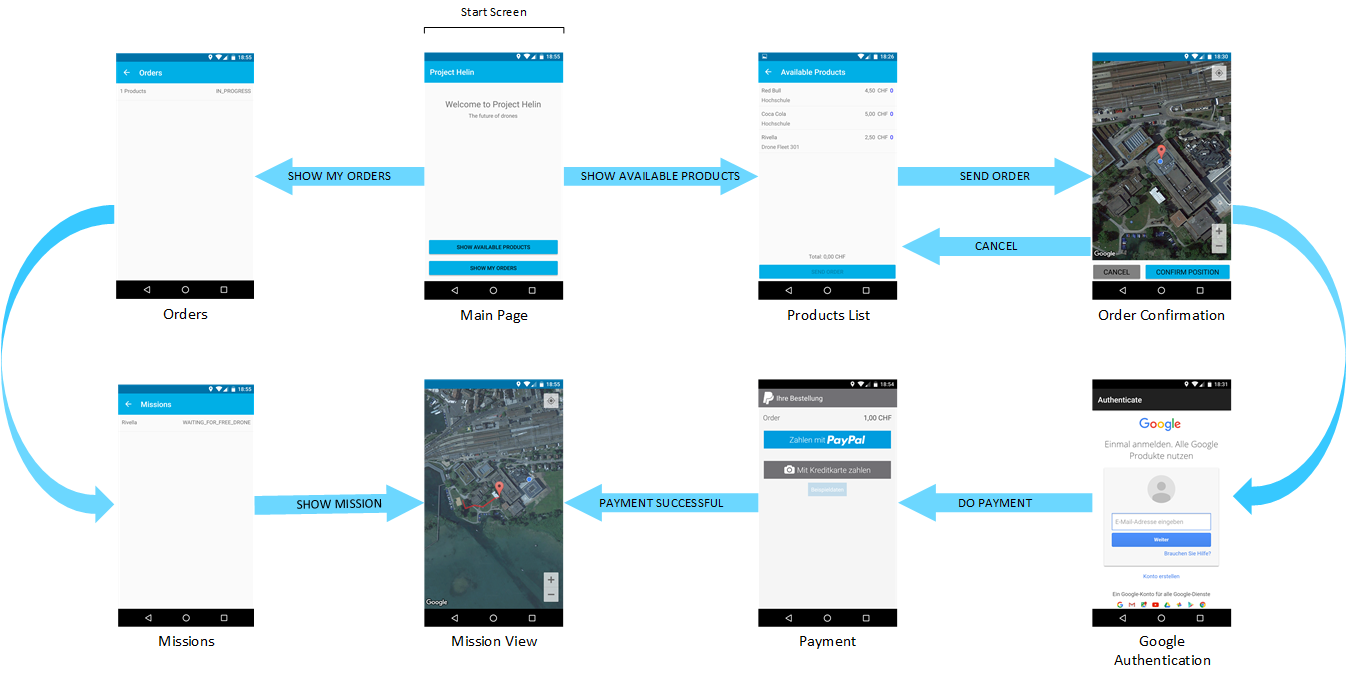
\includegraphics[width=0.8\paperheight] {images/customer-app-pages.png}
		\caption{Übersicht der Customer App mit allen Verknüpfungen zwischen den Screens}
		\label{fig:customer-app-flow}
	\end{figure}
\end{landscape}

\subsubsection{Verwendete Bibliotheken}
\begin{tabularx}{\textwidth}{|X|X|c|X|}
	\hline
	\textbf{Name} & \textbf{Verwendungszweck} & \textbf{Version} & \textbf{Lizenz} \\
	\hline \hline
	Paypal Forms & Paypal integration für Xamarin.Forms & 2.0.4 & MIT \\
	\hline 
	Xamarin Forms & Plattform übergreifende Komponente für Xamarin & 2.2.0.45 & \url{https://www.xamarin.com/license} \\
	Websocket.PCL & Plattformübergreifende Websocket Anbindung & 1.1.9 & MIT \\
	Newton.Json & Json zu Object mapper & 8.0.3 & MIT \\
	\hline 
\end{tabularx}


\subsection{Kommunikation}
Um die nichtfunktionalen Anforderungen im Bereich der Kommunikation zu erfüllen, wurde AMQP als Protokoll ausgewählt. Mit Messaging soll gewährleistet werden, dass die Verbindungswiederherstellung funktioniert. Die funktionale Anforderung des Missionsabbruchs wird somit soweit gedeckt, dass versucht wird die Verbindung aufrechtzuerhalten, sofern das Netz es erlaubt. Bei kurzen Netzunterbrüchen kann somit über das AMQP Protokoll eine Verbindung zur Drohne gewährleistet werden.

\begin{itemize}
	\item{\textbf{Verbindungsabbruch:} \\
		Gemäss den nicht funktionalen Anforderungen darf der Verbindungsabbruch keinen Einfluss auf die Mission haben. Um gemäss den funktionalen Anforderungen einen Missionsabbruch zu gewährleisten, wird versucht Unterbrüche so kurz wie möglich zu halten und einen automatischen Verbiundungsaufbau zu ermöglichen. Aus diesem Faktoren wird die gesamte Mission vor dem Start übertragen, damit sie ausgeführt werden kann. Einzelne Wegpunke sind somit nicht auf eine stabile Internetverbindung angewiesen, da die Route bereits von Anfang bekannt ist. Der Missionsabbruch ist ebenfalls gewährleistet - sofern die GSM Verbindung besteht. 
		\\
		Verbindungsabbrüche auf dem Mobiltelefon haben zweierlei Konsequenzen:	
		\begin{itemize}
			\item{\textbf{Mobiltelefon kann die Messages vom Server nicht empfangen:} \\
				Dieses Szenario wird durch das RabbitMQ abgefangen. Der Messaging Broker cached die Nachrichten solange bis der Consumer (Mobiltelefon) wieder verfügbar ist. Es besteht somit kein zusätzlicher Handlungsbedarf auf dem Onboard-App.
			}
			\item{\textbf{Messages vom Mobiltelefon zum Server können nicht gesendet werden:} \\
				In diesem Fall kann der Übertragungsfehler nicht durch RabbitMQ abgefangen werden. Der Broker hat vom Producer (Mobiletelefon) noch keine Nachricht bekommen. Aus diesem Grund wird producerseitig eine Exception geworfen, die darauf hinweist, dass die Verbindung unterbrochen ist. In diesem Fall wird die Nachricht in einem Queue zwischengespeichert. Sämtliche Folgenachrichten, die während des Verbindungsunterbruchs nicht übertragen werden können, werden ebenfalls in dieser Queue gespeichert. Sobald die Verbindung wieder besteht, werden die Nachrichten aus der Queue gesendet.
			}
		\end{itemize}
		Mit diesen Massnahmen ist ein guter Kompromiss aus Zuverlässigkeit und Aufwand entstanden. Alle missionskritischen Nachrichten können übertragen werden. Telemetriedaten sind von einem Verbindungsausfall ebenfalls nicht betroffen.
	}
	\item{\textbf{Verbindungswiederherstellung:}
		Aus den nicht funktionalen Anforderungen ist zu entnehmen, dass bei einem Verbindungsunterbruch ein Reconnect statt findet. Dieser Reconnect soll, sobald die Verbindung im GSM Netz wieder besteht nicht länger als 30s dauern. \\
		Bei der Konfiguration von AMQP bestanden mehrere Möglichkeiten. Einersetis war der bekannte Backoff Algorithmus eine Option. Dieser Algorithmus arbeitet nach einem incrementellen Prinzip. Je länger der Unterbruch dauert, desto länger dauert es bis er die Verbindung wieder versucht aufzubauen. Auf der anderen Seite stand ein einfacher Interval-Algorithmus. Dieser versucht alle drei Sekunden die Verbindung wiederherzustellen, bis zum erfolgreichen Verbindungsaufbau. Mit diesen Erkenntnissen haben wir folgende Messung gemacht:
		\begin{center}
			\begin{tabular}{|r|r|}
				\hline
				\textbf{Backoff} & \textbf{Interval 3s} \\
				\hline
				17 & 7 \\
				7 & 7 \\
				9 & 7 \\
				11 & 7 \\
				10 & 7 \\
				\hline
				% TODO: Kommentar noch: Anzahl Sekunden bis zum Verbindungsaufbau
			\end{tabular}
		\end{center}
		Aus diesen Erkenntnissen standen beide Möglichkeiten offen, denn beide erfüllen die Anforderungen und haben somit auch keine Auswirkungen auf die Qualität. Am Ende wurde bewusst auf den BackOff Algorithmus gesetzt. Der Backoff Algorithmus benötigt zwar deutlich länger für einen Reconnect als das fixe Zeitinterval. Die hetrogene Verteilung der Wiederverbindungszeiten spricht aber für den Backoff Algorithmus. Sollte es zu Probleme auf der Serverseite kommen, so werden nicht alle Geräte gleichzeitig einen Reconnect probieren - der Reconnect passiert somit gestaffelt. Dies bringt zusätzlich Stabilität ins System.}
	\item{\textbf{Android Process Lifecycle:} \\
		Da die OnboardApp auf einem Android Betriebssystem läuft, mussten gewisse Voraussetzungen geprüft werden. Im Grund kann davon ausgegangen werden, dass die Applikation immer im Vordergrund steht. Es ist doch sehr unwahrscheinlich, dass die Appliaktion in den Hintergrund rückt, weil eine andere Applikation verwendet wird. \\
		Laut Android Dokumentation ist das Verhalten einer Applikation im Hintergrund nicht deterministisch \cite{androidGuide}. Sollte eine Applikation im Hintergrund gewisse Garantien haben, so muss von einem Service und der spezifischen Implementierung eines Services gesprochen werden. Im Fall der OnboardApp und den getroffenen Annahmen, wurde davon abgesehen, da die Applikation während des Fluges nicht gewechselt wird.
	}
	\newpage
\end{itemize}

\section{Qualitätsmassnahmen und Messungen}

\subsection{Statistiken}

Folgende Statistiken wurden am Ende der Arbeit erstellt um einen Eindruck der Grösse und der Qualität des Projektes zu erhalten.

\begin{figure}[h]
	\centering
	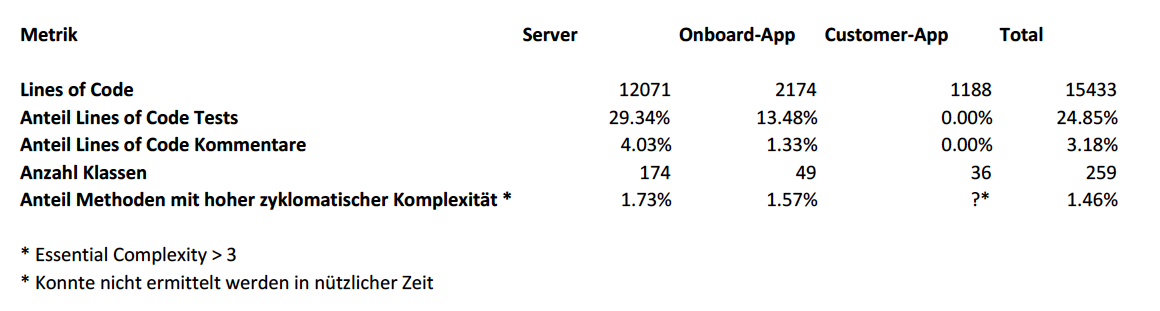
\includegraphics[width=1.0\textwidth] {images/code-metrics.png}
	\caption{Code Metriken nach Abschluss der Arbeit}
	\label{fig:code-metrics}
\end{figure}

\subsection{Continous Integration}

Als Build-Server haben wir TeamCity verwendet. Dort waren alle Projekte (ausser Customer-App) jeweils mit einem Build für den develop- und master-branch eingerichtet. Alle Builds führten die nötigen Tests aus und produzierten ein entsprechendes Artifact für das Deployment. Das Deployment für den Server wurde ebenfalls automatisiert.

\subsection{Testing}

Je nach Plattform wurden andere Formen von Tests durchgeführt. 

\subsubsection{Server}

Auf dem Server wurden vor allem E2E- und Integration-Tests verwendet um die Funktionalität zu prüfen. Wir haben uns bewusst gegen Unit-Tests entschieden, da auf dem Server nur wenig Logik zu finden ist, die nicht von der Datenbank oder der RabbitMQ-Connection abhängt. Unit-Tests hätten deswegen nur einen ganz kleinen Teil der Anwendungen abdecken können und wären in den meisten Fällen sehr aufwändig gewesen. Sogar die Routenberechnung konnte nicht mit Unit-Tests abgedeckt werden, da ein Teil der Berechnung auf der Datenbank stattfindet und somit nur Integrationtests einen Sinn ergeben.\\

Wir haben darauf geachtet, dass immer nur die minimale Integrationsstufe gewählt wurde. Für die Simulation eines Benutzers (E2E) wurde Selenium verwendet, das widerum einen Firefox Browser verwendet. Für die Api- und Messaging-Controller wurden Integrationtests verwendet, welche den Server ohne Browser verwenden.\\

Es wurde eine durchschnittliche Testabdeckung von 72\% über das ganze Projekt erreicht. In wichtigen Packages liegen diese aber meist über 85\%.

\subsubsection{Onboard-App}

Beim Onboard App wurden nur Unit-Tests ausgeführt. 


\subsection{Code Reviews}



\newpage
\section{Flugrouten}
Die zentrale Aufgabe des Projektes ist es Drohnen zu verwalten, die sich in einem geografischen Gebiet autonom und sicher bewegen können. 
Dieses Gebiet, beispielsweise die HSR (siehe Abb. \ref{fig:campus-hsr}) kann Hindernisse wie Gebäude oder Bäume enthalten, welche um- oder überflogen werden müssen. \\

\begin{figure}[H]
	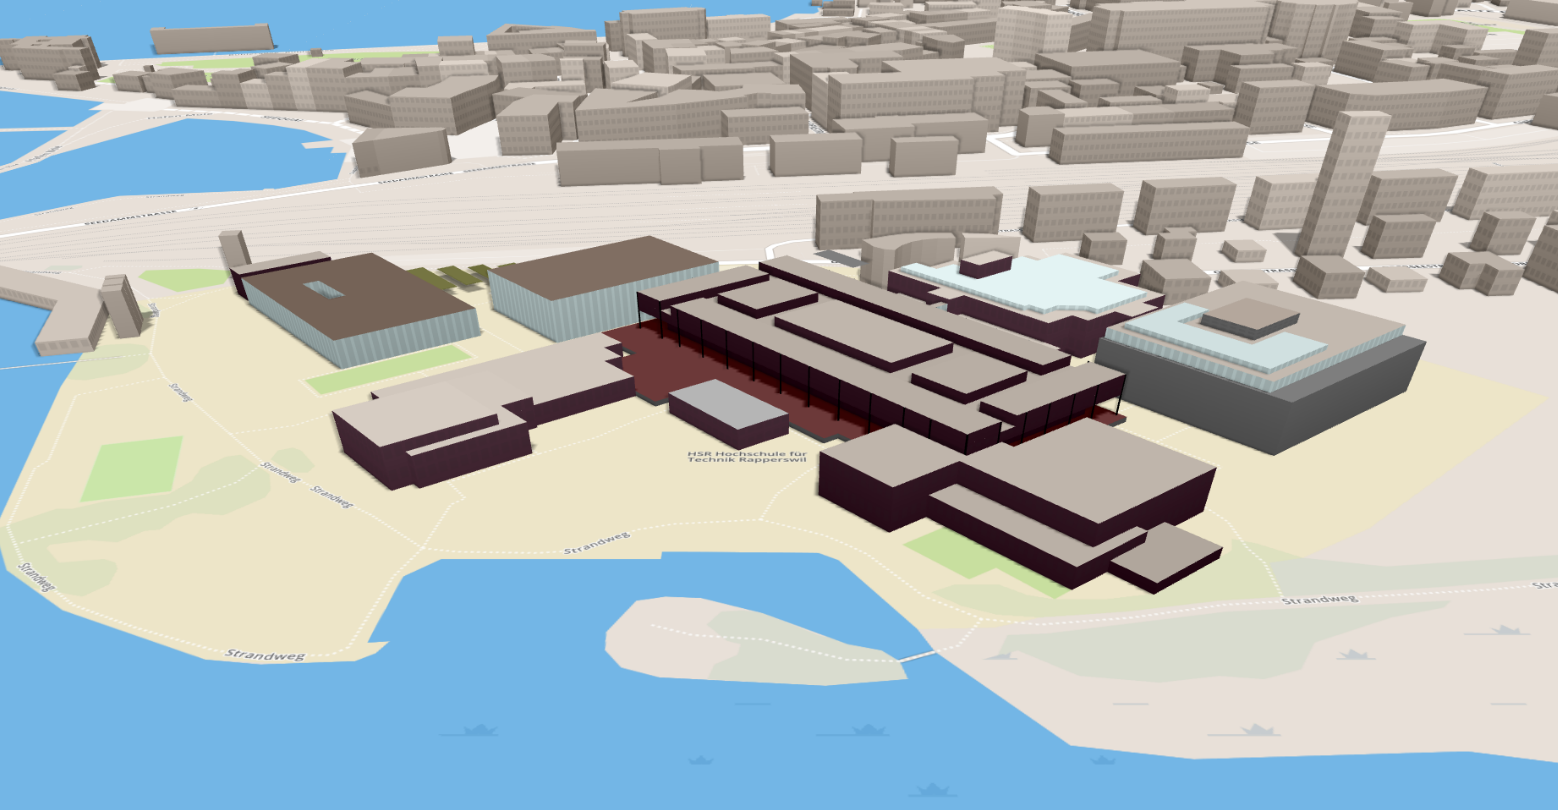
\includegraphics[width=1.0\textwidth]{images/routing/topology_example.png}
	\caption{Topologische Ansicht des Campus HSR}
	\label{fig:campus-hsr}
\end{figure}

\subsection{Das Zonen Model}
Um Kollisionen mit statischen Objekten zu vermeiden und sichere Flugwege zu erhalten, wurde ein Zonen Model eingeführt. Dieses ermöglicht dem Anbieter zu definieren, wo geflogen werden kann und wie hoch dort geflogen werden muss. Die Abbildung \ref{fig:demo-project} zeigt die Benutzeroberfläche für die Zonendefinition anhand des HSR-Campus.

\begin{figure}[H]
	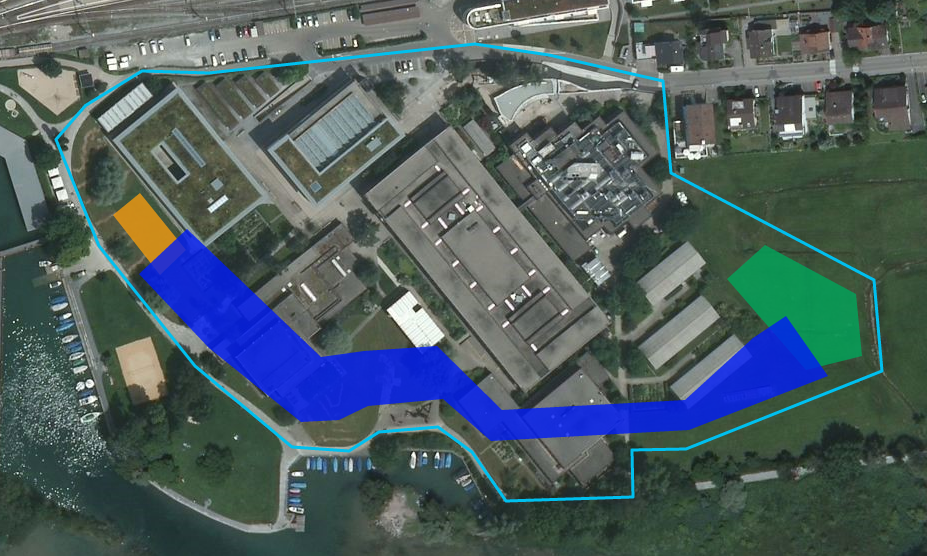
\includegraphics[width=1.0\textwidth]{images/routing/simpleProject_example.png}
	\caption{Einfaches Demo Projekt an der HSR}
	\label{fig:demo-project}
\end{figure}
Jedes Polygon bildet eine Zone ab. Jede Zone enthält eine Flughöhe sowie einen Typ:
\begin{itemize}
	\item{\textbf{Order Zone:} Zone in welchem die Produkte des Projekts bestellt werden können. (\textit{hell blauer Rahmen})}
	\item{\textbf{Loading Zone:} Zone in welcher die Drohne beladen wird. (\textit{orange})}
	\item{\textbf{Delivery Zone:} Zone in der geliefert und geflogen werden darf. (\textit{grün})}
	\item{\textbf{Flight Zone:} Zone in der nur geflogen aber nicht geliefert werden darf. (\textit{blau})}
\end{itemize}

\subsection{Von der Zone zum Graph}
Normalerweise wird eine Routenberechnung mit Hilfe eines Graphen durchgeführt, der durch die möglichen Wege (z.B. Strassen) definiert ist. Da die Zonen aber eine Fläche bilden, mussten diese zuerst in einen Graphen umgewandelt werden. \\

Folgende Lösungsmöglichkeiten wurden evaluiert:

\subsubsection{Erstes Konzept: Direkte Route}
Dieses Konzept umfasste den Ansatz den Start und den Endpunkt direkt zu verbinden, und bei einem Verlassen des Polygons dem Rand zu folgen (siehe Abb. \ref{fig:first-concet-routing}).

\begin{figure}[H]
	\centering
	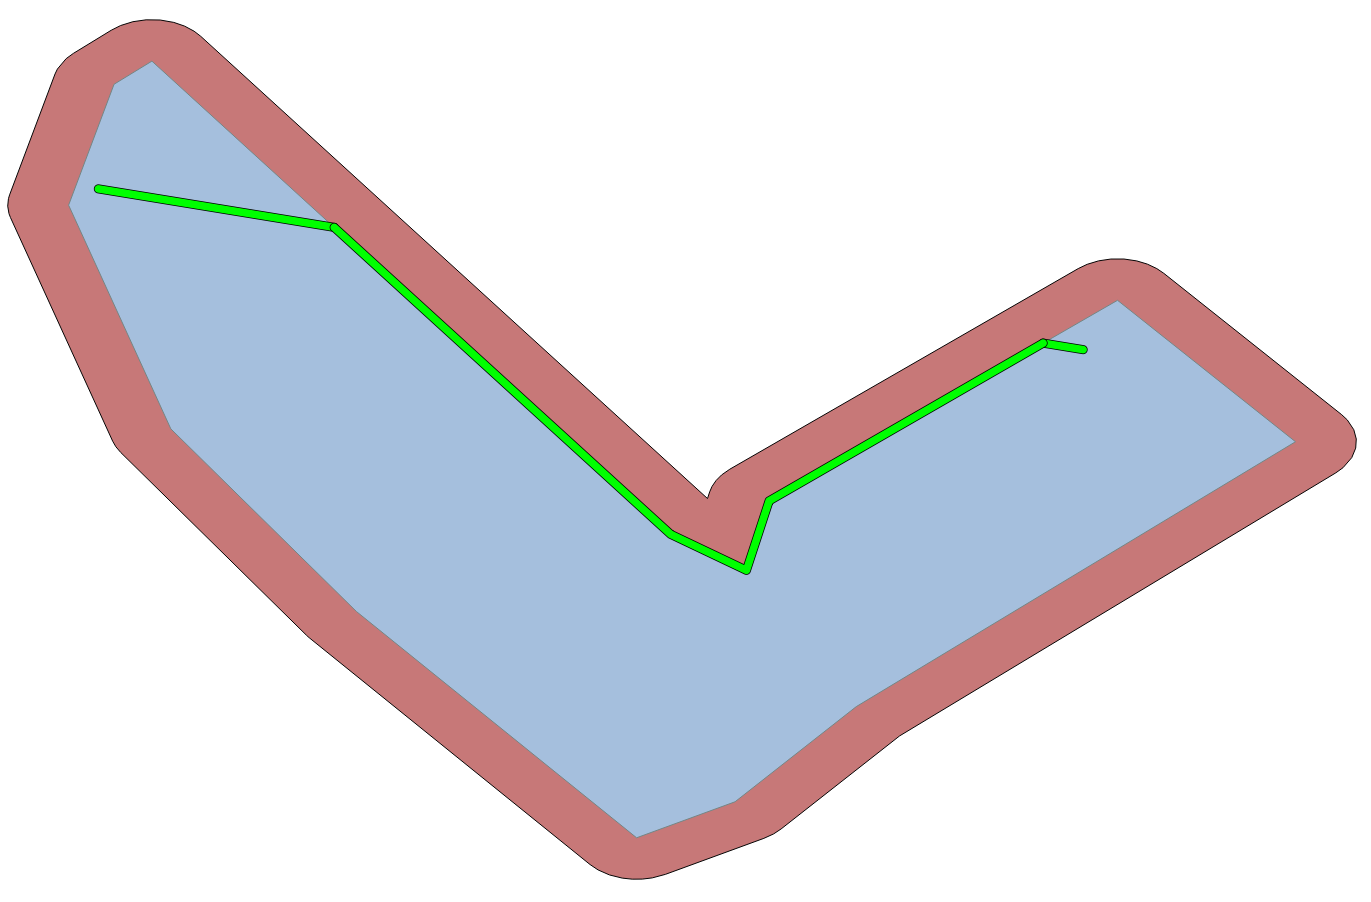
\includegraphics[width=0.8\textwidth]{images/routing/firstSolution.png}
	\caption{Erstes Konzept}
	\label{fig:first-concet-routing}
\end{figure}
Es wurde ausserdem ein Rand (\textit{Rot}) hinzugefügt. Diese Massnahme wurde getroffen, um allfällige GPS Ungenauigkeiten zu berücksichtigen.\\

Der Nachteil dieser Lösung zeigt sich bei grösseren Polygonen, wo unnötigerweise dem Rand entlang geflogen wird, obwohl ein Flug durch die Mitte viel sicherer wäre.
\newpage
\subsubsection{Zweites Konzept: Visibility Graph}
Das nächste Konzept orientiert sich an einem 'Visibility Graphen'. 
\cite[]{IEEEPaper} 

\blockquote{Using visibility graphs for determining the shortest path is very practical and intuitive. The visibility graph of a set of nonintersecting polygonal obstacles in the plane is an undirected graph whose vertices are the vertices of the obstacles and whose edges are pairs of vertices such that the open line segment between each two vertices does not intersect any of the obstacles.}

In unserem Fall haben wir den Gedanken umgedreht. Wir haben den Graphen in einem Polygon mit potentiellen Löchern berechnet. Diese Löcher stellen Enklaven für Bäume oder Gebäude dar. Das Konzept ist aber identisch, angewendet auf unser Beispiel Polygon ergibt sich folgende Abstraktion:
\begin{figure}[H]
	\centering
	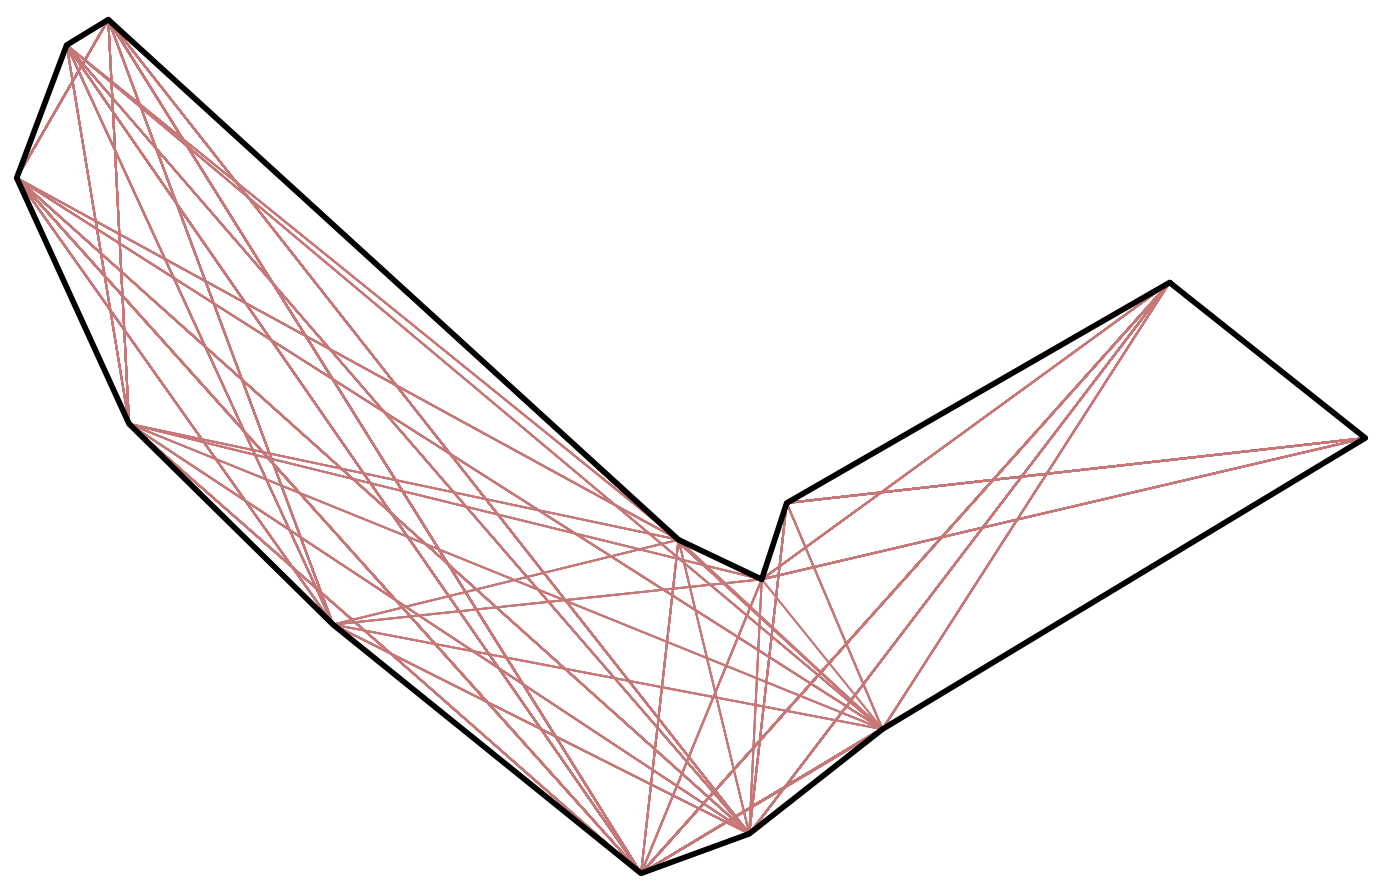
\includegraphics[width=0.8\textwidth]{images/routing/visibilityGraph.png}
	\caption{Visibility Graph in einer Flugzone}
	\label{fig:visibility-graph}
\end{figure}
Wie in der Abbildung \ref{fig:visibility-graph} gezeigt wird, verlaufen deutlich weniger Flugrouten entlang der Kante des Polygons. \\
Dies ist eine deutliche Verbesserung gegenüber dem ersten Konzept. Der Nachteil ist, dass die innere Ecke des L-förmigen Polygons sicher angeflogen wird, da es die vermeintlich kürzeste Route in einem nächsten Schritt darstellen würde. Aus diesem Grund haben wir uns gegen den Einsatz dieses Konzepts entschieden.\\

\subsubsection{Drittes Konzept: Straight Skeleton}
Da die Pfadfindung von \Gls{UAV} bereits ein weit erarbeitetes und erforschtes Gebiet ist, waren wir der Überzeugung, dass bereits verwendete Konzepte vereinfacht und abstrahiert werden konnten, um unser Problem zu lösen. Während vollständig autonome Drohnen an Hindernissen vorbei navigieren müssen, können wir uns auf einen bestehenden Flugkorridor verlassen.
\blockquote{The idea behind this method is to assign a function similar to the electrostatic potential to each obstacle and then derive the topological structure of the free space in the form of minimum potential valleys. The robot is positioned at the start point, and then the goal generates a strong attractive force. By the action of the force, the robot moves along the steepest descent of the potential to the goal, at the same time the obstacle generates a repulsive force to keep robot away from colliding with them} 

Die Kernaussage des zitierten Papers \cite[]{SkeletonUAV} ist, dass ein Pfad den grösstmöglichen Abstand zu den Hindernissen aufweisen soll. Auf unseren Fall übertragen, sind die Polygonränder die Hindernisse. Somit muss gewährleistet werden, dass die Drohne den grössten Abstand zu den Rändern aufweist. Aus diesem Grund erscheint diese Lösung für uns sehr geeignet, da sie mittenbetonte Routen vorschlägt. \\
\begin{figure}[H]
	\centering
	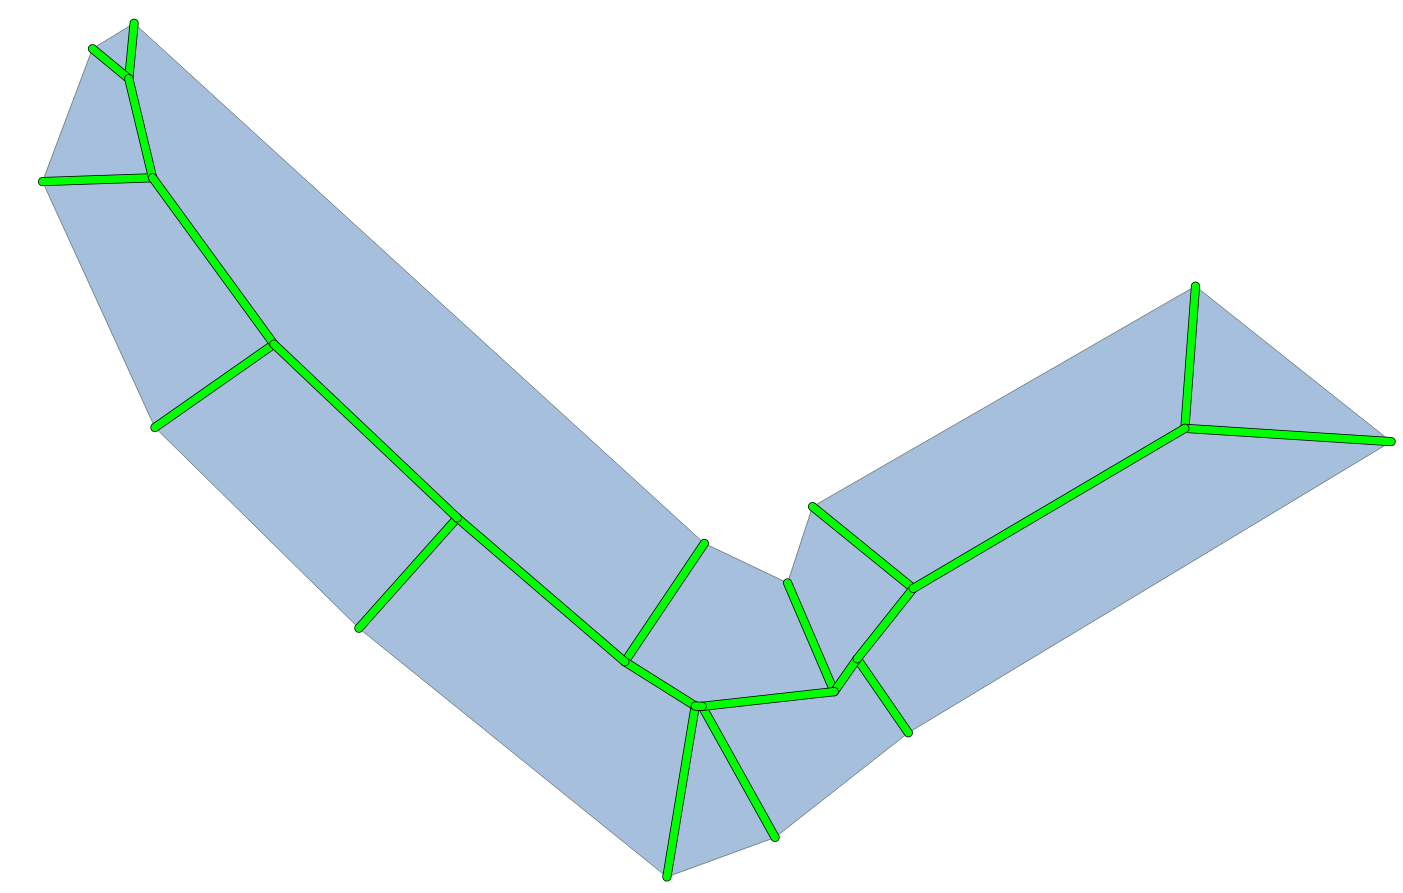
\includegraphics[width=0.8\textwidth]{images/routing/skeleton.png}
	\caption{Skeleton in Polygon}
	\label{fig:skeleton-in-polygon}
\end{figure}
Die Abbildung \ref{fig:skeleton-in-polygon} illustriert die Lösung mithilfe eines Skeletons. Dieses Konzept kann nachvollzogen werden, indem man sich das Polygon 3-dimensional vorstellt und dann  von der Mitte aus, parallel zu den Kanten schneidet. Der entstandene Grat ist hier als Linie sichtbar und wird als Skeleton bezeichnet. Der Felkel-Algorithmus, welcher dieses Skeleton aus einem 2-dimensionalen Polygon berechnet ist bereits in \Gls{CGAL} implementiert \cite{SkeletonCGAL} und war uns im weiteren Verlauf des Projektes von grossem Nutzen.\\






\subsection{Routing Algorithmus}
Nach der Herleitung des Graphen aus den Zonen, musste nun der passende Algorithmus gefunden werden, um einen möglichst effizienten Weg von A nach B zu finden. Es kamen vier Algorithmen in Frage, wobei ein Algorithmus sich als besonders geeignet herausstellte.
\begin{itemize}
	\item{\textbf{BFS:} (\textit{Breadth-first search}) Die Breitensuche durchsucht einen Baum in der Breite. Sie bringt garantiert eine Lösung, wenn eine Lösung vorhanden ist und kann problemlos mit Zyklen im Graph umgehen. Bei der Lösung handelt es sich aber nicht um de 'optimale Lösung' (kürzester Pfad). Die Lösung liefert den Pfad mit den wenigsten Knoten. \cite{AiClass}}
	\item{\textbf{DFS:} (\textit{Depth-first search}) Die Tiefensuche fängt an einem Knoten an und arbeitet sich dann in die Tiefe. Das Problem ist, dass sie sehr anfällig auf Zyklen ist und ohne weitere Hilfsmittel (loop detection oder pruning) nicht terminieren kann. \cite{AiClass}}
	\item{\textbf{A-Star:} Der A-Star Algorithmus arbeitet mit einer Heuristik und funktioniert effizienter als die zwei bereits genannten Algorithmen. Allerdings ist der Aufwand für die Umsetzung deutlich höher. \cite{AiClass}}
	\item{\textbf{Dijkstra:} Der Dijkstra-Algorithmus ist ebenfalls ein klassischer Graphpropagierungsalgorithmus. Der Vorteil ist, dass er grundsätzlich ohne Heuristik auskommt und robust mit Zyklen umgehen kann. Ausserdem können die Kanten mit einem Gewicht versehen werden und dadurch, der kürzeste Weg berechnet werden.}
\end{itemize}
Wir haben uns für den Dijkstra Algorithmus entschieden. Er liefert ohne Metrik eine ähnliche Lösung wie die BFS-Suche, kann aber im Nachhinein erweitert werden um effizientere Routen zu liefern.

\subsection{Höhenhandling}
Damit die Route 2-Dimensional berechnet werden kann, werden die Höhen erst zum Schluss berücksichtigt. Das Höhenhandling bildet den abschliessenden Schritt bei der Berechnung einer Route und wird in zwei Schritten durchgeführt:

\begin{itemize}
	\item{\textbf{Eindeutigkeit der Höhe:} In einem ersten Schritt werden die Zonen nach Höhe absteigend sortiert und Überlagerungen zugunsten der höheren Zone entfernt.}
	\item{\textbf{Bestimmen der Zugehörigkeit des Knotens:} Angefangen bei der höchsten Zone werden die Liniensegmente mit der jeweiligen Zonenhöhe versehen. Bei Linien, welche die Zone verlassen, wird ein Punkt am Schnittpunkt eingefügt.}
\end{itemize}
\begin{figure}[h]
	\centering
	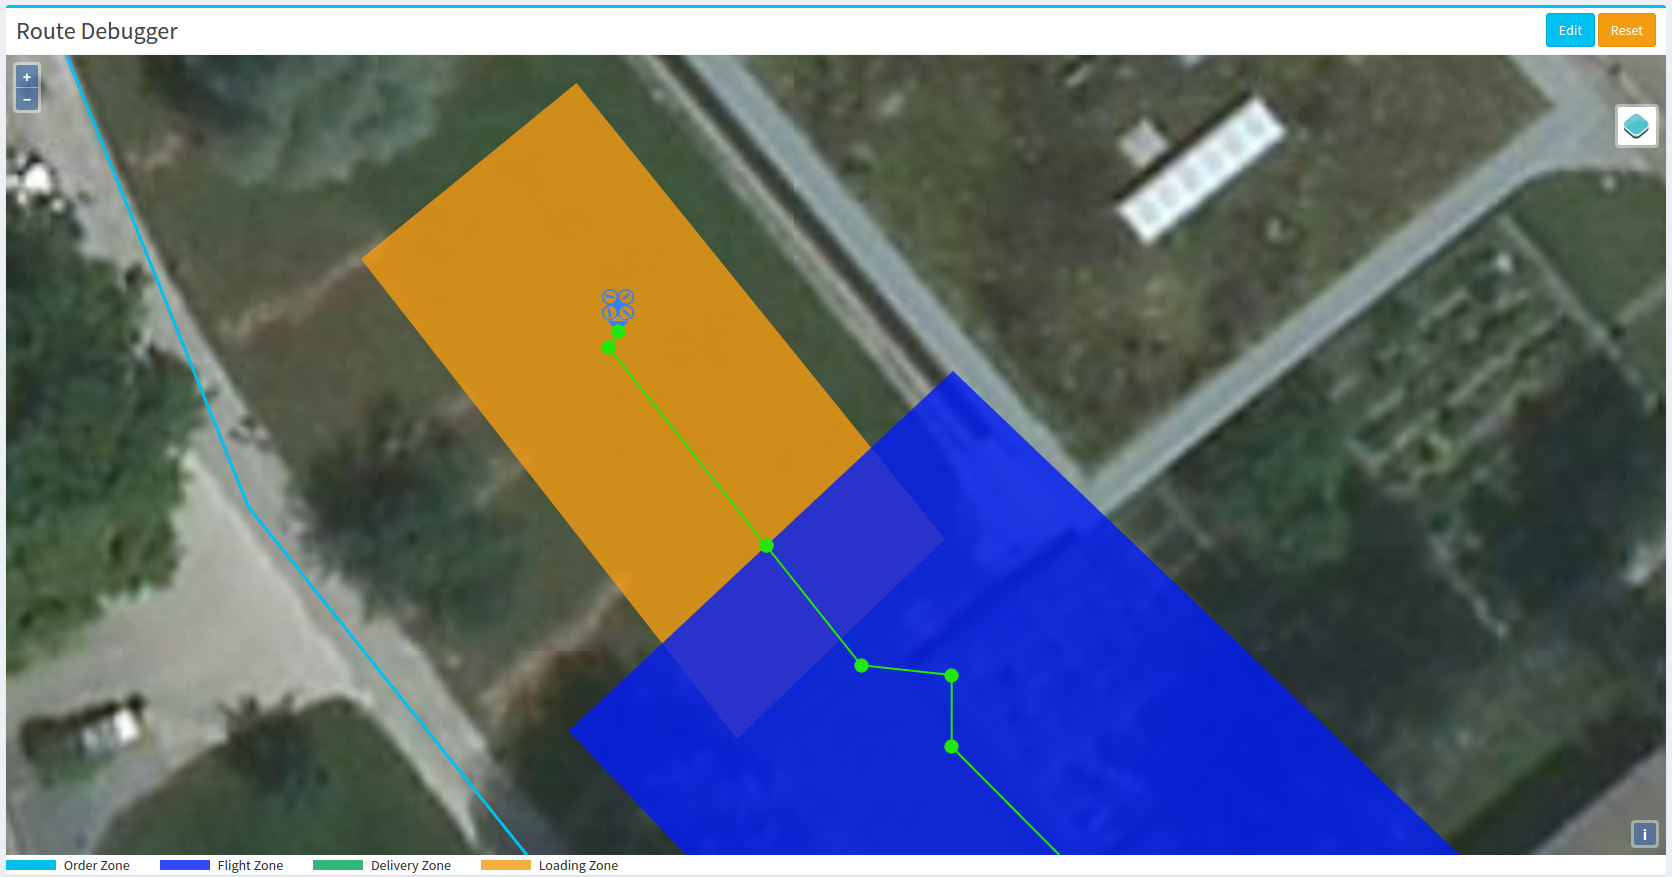
\includegraphics[width=1.0\textwidth]{images/routing/height_example.png}
	\caption{Beispiel der Höhe am Übergang zweier Polygone}
	\label{fig:polygon-border-example}
\end{figure}
Wie gemäss der Abbildung \ref{fig:polygon-border-example} ersichtlich ist, ist trotz des langen geraden Pfades zwischen den zwei Zonen ein Punkt eingezeichnet. Im Grunde sind es zwei Punkte, die für den Wechsel der Flughöhe verantwortlich sind.
\newpage
\subsection{Wahl der Rückroute}
Das Bilden der Rückroute erfolgt in einem sehr einfachen Verfahren. Bei der aktuellen Lösung werden Start und Endpunkt mit der dazugehörigen Aktion versehen. Im Falle des Endpunktes ist es in unserem Fall der Abwurf.
\\
Nun kann dieser Pfad genommen, umgedreht und angehängt werden, wobei der letzte Punkt entfernt wird. So ist garantiert, dass die Drohne den gleichen Rückweg wie Hinweg verwendet um die Mission zu erfüllen. Diese Liste wird verwendet um dem Autopiloten mit Wegpunkten zu versorgen.

\chapter{Versuchsaufbau}

\section{Einleitung}

Um die vom Team erstellte Plattform auch unter realen Bedingungen testen zu können, wurde ein Versuchsaufbau mit zwei Drohnen erstellt, die es ermöglichen Produkte zu transportieren und über dem Kunden mit einem Fallschirm abzuwerfen. Der Aufbau der Drohnen beinhaltete die Zusammenstellung der passenden Komponenten, den Zusammenbau der Drohnen und die Planung und Erstellung von zusätzlichen Halterungen für die obengenannten spezifischen Anforderungen.\\


<<<<<<< HEAD
\begin{itemize}

\item Flight-Controller muss \Gls{MAVLink} Protokoll unterstüzen
\item Onboard-App muss über MAVLink mit dem Flight-Controller verbunden sein. (Über USB oder eine Funk-Telemetrieverbindung.)
\end{itemize}

\section{Multicopter Hardware}

\section{Teile-Liste}

\begin{tabularx}{\textwidth}{|X|l|l r|}
	\hline
	\textbf{Bezeichnung} & \textbf{Bezugsquelle} && \textbf{Preis}\\
	\hline \hline
	DJI F450 ARF Kit & conrad.ch & CHF &229.95 \\\hline
	DJI F450/F550 Landegestell & conrad.ch & CHF &24.95 \\\hline
	3DR Pixhawk & 3dr.com & USD& 199.99 \\\hline
	3DR uBlox GPS with Compass Kit & 3dr.com & USD &89.99 \\\hline
	Pixhawk external LED and USB & 3dr.com & USD & 20.00 \\\hline
	FrSky X8+ Radio Transmitter & 3dr.com & USD & 89.99 \\\hline
	FrSky X8R Receiver & hebu-shop.ch & CHF & 39.95 \\\hline
	Delock Micro USB OTG Kabel & digitec.ch & CHF &15.90 \\\hline
	Multistar High Capacity 4S Akku (2x) & hobbyking.com & USD& 50.50 \\\hline
	APM Flight Controller Damping Platform & hobbyking.com & USD& 2.69 \\\hline
	Smartphone und GPS Halterung & eigener 3D-Print & CHF &27.50\\\hline
	Abwurfvorrichtung & eigener 3D-Print & CHF &25.50\\\hline
	Hitec Super Servo S-Bec (Stromversorgung Servo) & brack.ch & CHF &13.90\\\hline
	Tactic TSX10 (Servo für Abwurf) & brack.ch & CHF & 14.90\\\hline
	Kleinmaterial & diverse & CHF & 50.00\\\hline
		\hline
	\textbf{Total} & & \textbf{CHF/USD} & $\boldsymbol{\approx 900.00}$\\\hline
\end{tabularx}

\subsection{Frame und Antrieb}

Der Frame, die Motoren und ESCs wurden als Kit gekauft. Es handelt sich dabei um ein DJI Flamewheel 450 Frame mit DJI 2312 960kV Motoren und ESeries 420 20A ESCs. Dieses Kit ist weltweit gut verfügbar und deshalb ideal geeignet um einen Versuchsaufbau zu erstellen.

\begin{figure}[h]
\centering
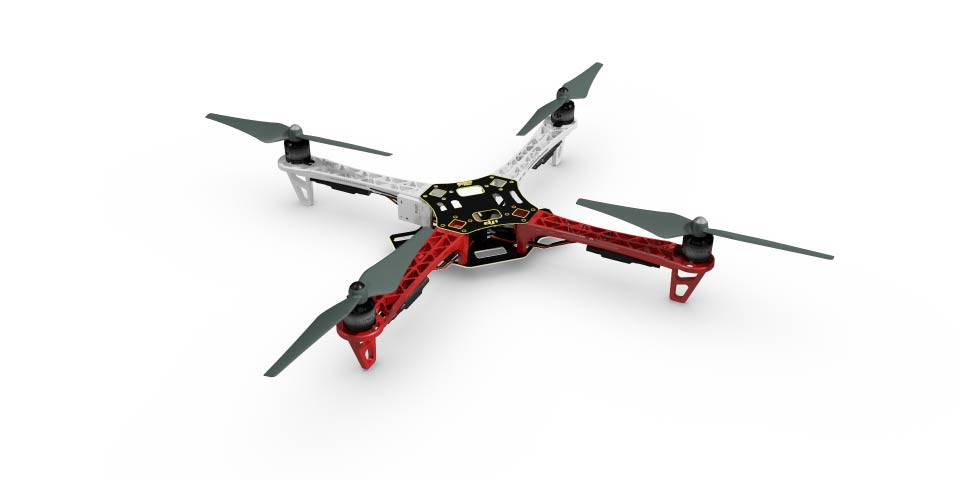
\includegraphics[width=0.9\textwidth] {images/hardware/f450.jpg} 
\caption{DJI F450 Flamewheel Kit}
\label{fig:f450}
\end{figure}


\subsection{Flight-Controller}

Der Flight-Controller ist das Herzstück eines Multicopters. Im Unterschied zu anderen ferngesteuerten Fahr- und Flugzeugen kann ein Multicopter nur über ein Fly-by-Wire System kontrolliert werden. Das heisst alle Befehle, die von der Fernbedienung gesendet werden, müssen interpretiert und umgewandelt werden, damit die Motoren eine Bewegung in die gewünschte Richtung erzeugen können. In Kombination mit einem GPS Modul (Abb. \ref{fig:gps-module}) ermöglich der Controller verschiedene Flugmodi, wie beispielsweise das Schweben an einem Punkt oder automatisches Abfliegen von Wegpunkten.

Als Flight-Controller setzen wir ein Pixhawk ein. Es ist sehr vielseitig und kann gut mit zusätzlichen Sensoren erweitert werden, ausserdem unterstützt es gängige Firmwares, die auch auf günstigeren Controllern laufen. Als Firmware für das Pixhawk setzen wir ArduCopter ein, da sie komplett Open-Source ist und auch bei vielen anderen Projekten eingesetzt wird. Sie unterstützt ausserdem das \Gls{MAVLink} Protokoll.

\begin{figure}[h]
\centering
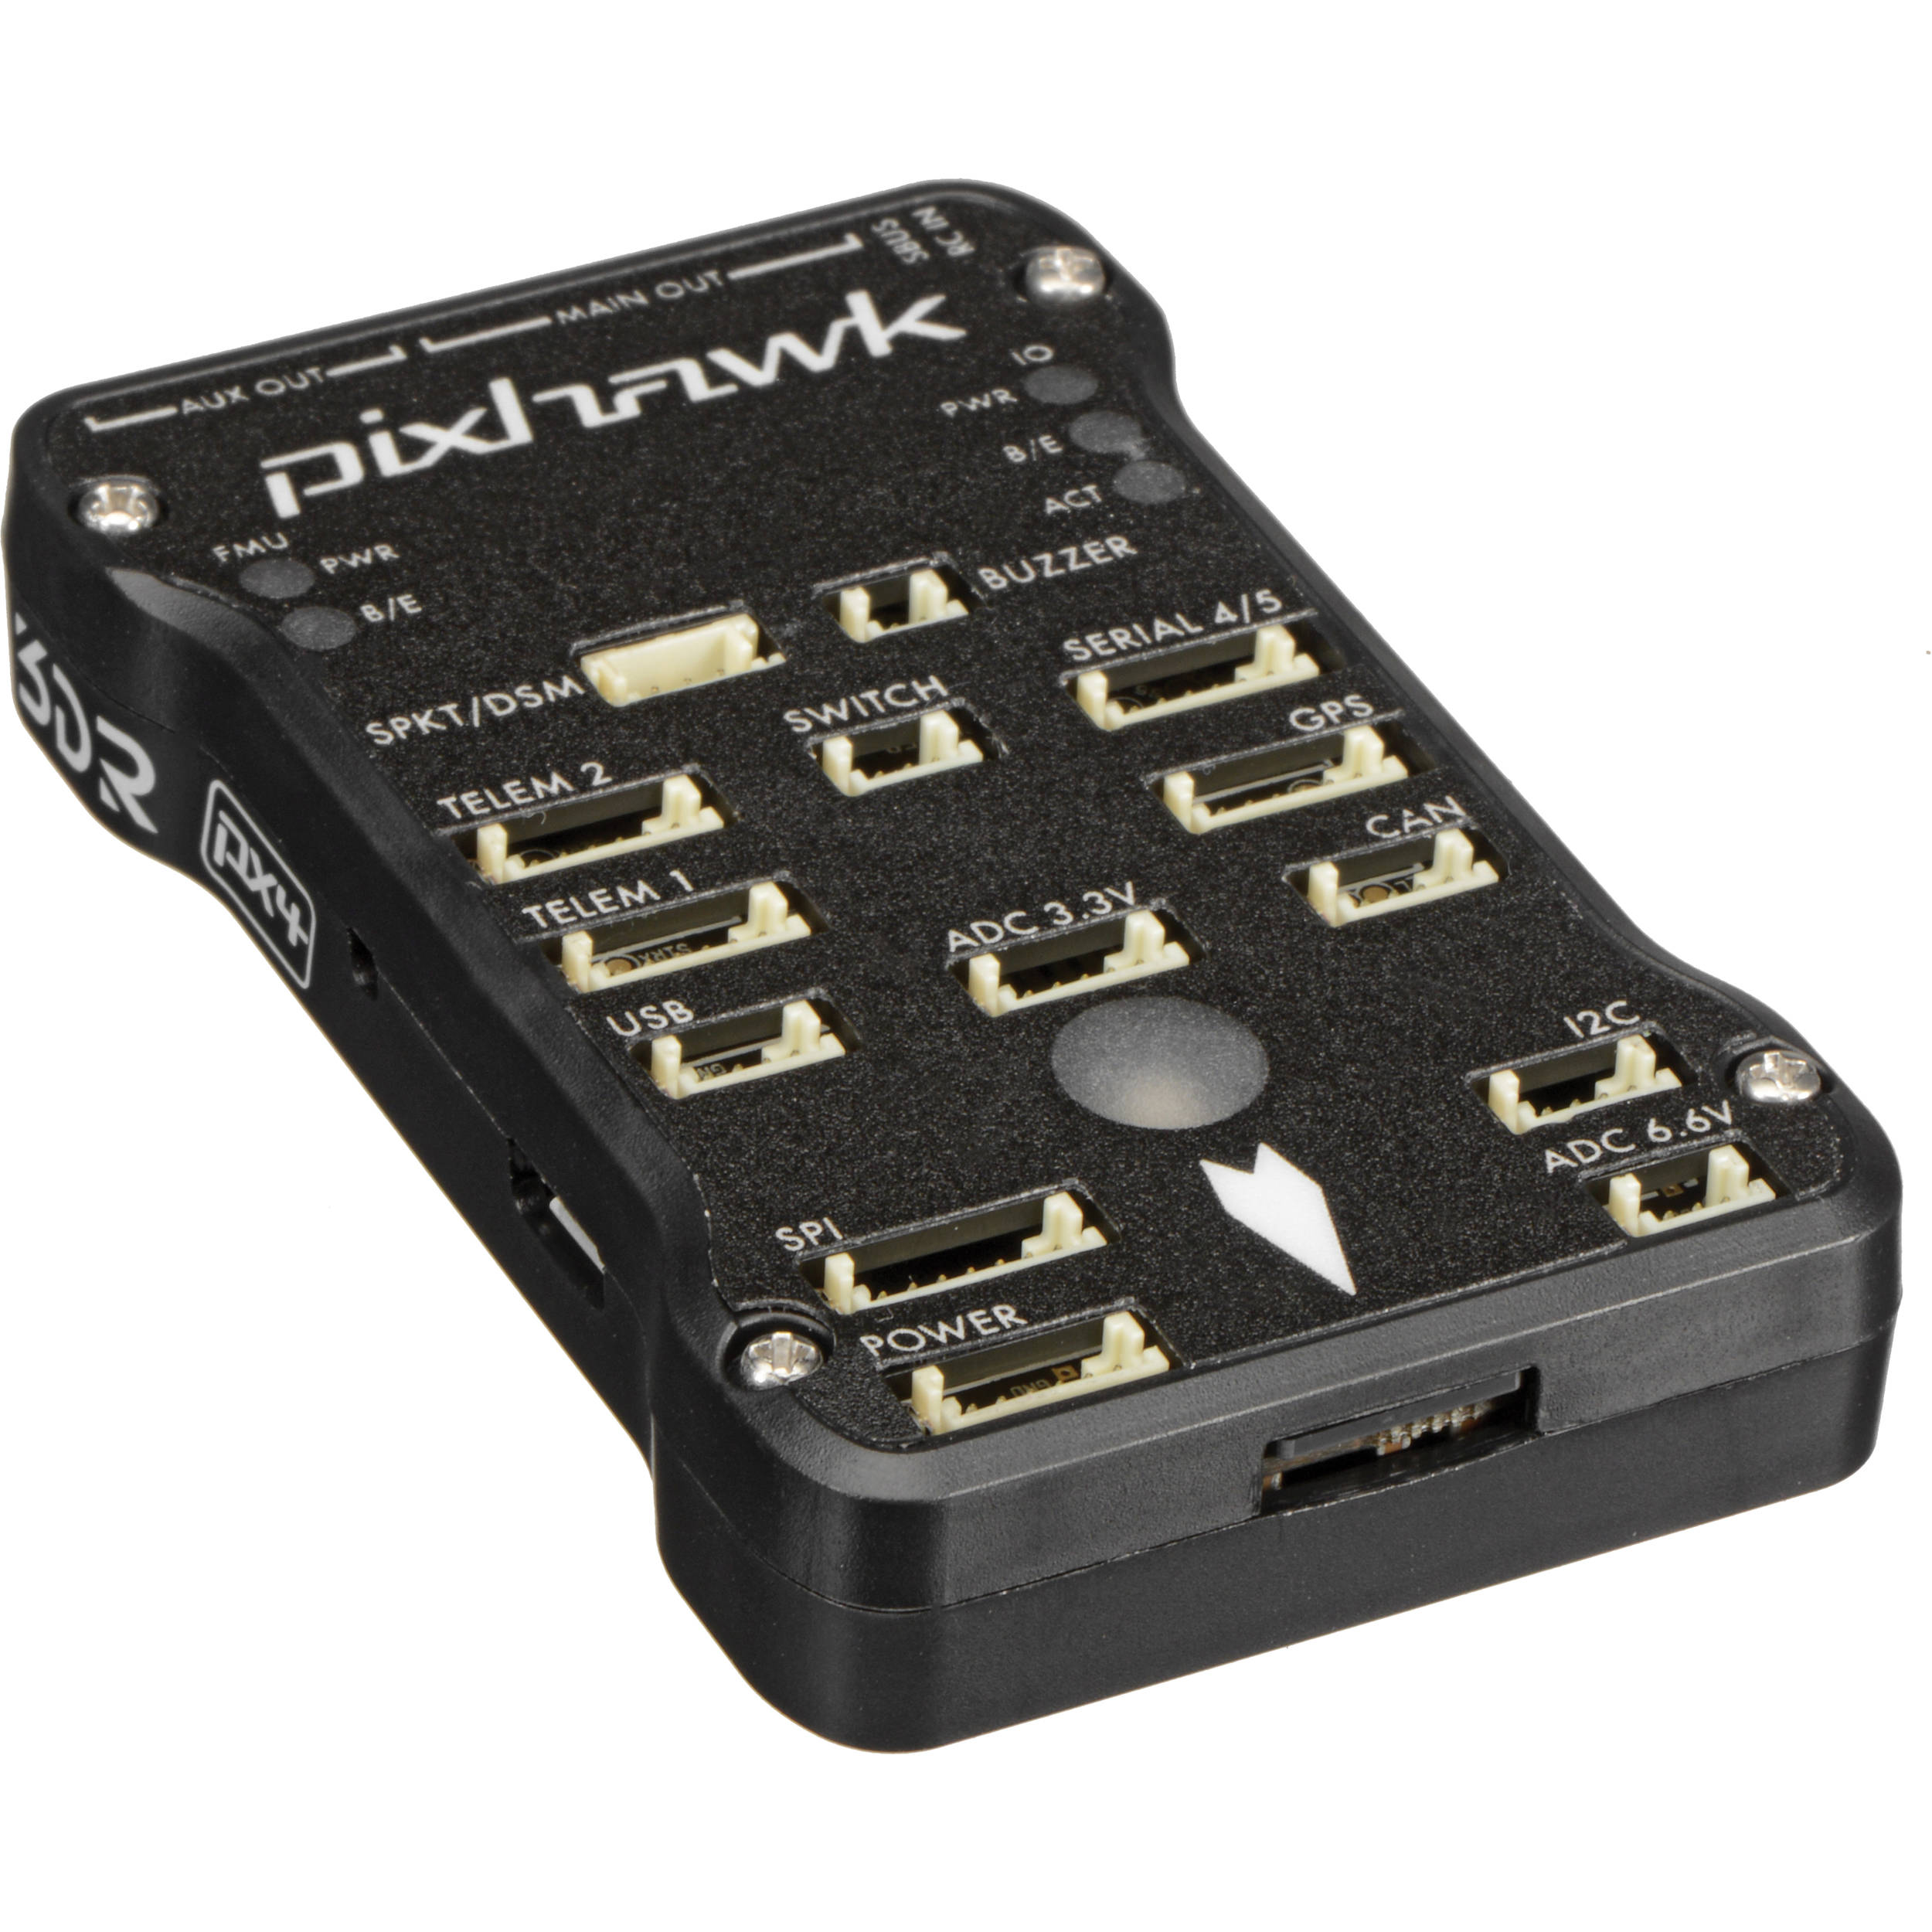
\includegraphics[width=0.3\textwidth] {images/hardware/pixhawk.jpg} 
\caption{Pixhawk Flight-Controller}
\label{fig:pixhawk}
\end{figure}

\begin{figure}[h]
\centering

\includegraphics[width=0.3\textwidth] {images/hardware/gps-module.jpg} 
\caption{GPS-Modul für Pixhawk}
\label{fig:gps-module}
\end{figure}

\subsection{Ausbaustufen}

Während des Projekts wurde die Hardware laufend den Bedürfnissen angepasst. Daher sind mehrere Versionen der Drohne entstanden, die für die Versuche genutzt wurden und geholfen haben Risiken früh auszuschliessen.

\subsubsection{Version 1}

\begin{figure}[H]
\centering
\includegraphics[width=0.4\textwidth] {images/hardware/prototype1.jpg}
\caption{Erster Prototyp ohne Landegestell und ohne Smartphone}
\label{fig:prototyp-1}
\end{figure}

Um das Zusammenspiel der Hardwarekomponenten zu testen und erste Erfahrungen mit dem GPS und den verschiedenen Flugmodi zu sammeln, wurde in der ersten Iteration nur die Drohne in einem minimal Flugzustand aufgebaut.

\subsubsection{Version 2}

\begin{figure}[H]
\centering
\includegraphics[width=0.4\textwidth] {images/hardware/prototype2.jpg}
\caption{Drohnen Aufbau mit Smartphone}
\label{fig:prototyp-2}
\end{figure}

Um die Risiken R08 (Ardupilot Handhabung) und R09 (Ardupilot API) frühzeitig auszuschliessen (siehe Tabelle \ref{table:risk-table}), wurde das Smartphone provisorisch auf die Drohne montiert, und mit einem ersten Prototypen der Onboard-App getestet. \\
Nach dem Test wurde uns klar, dass eine Befestigung für das Smartphone erarbeitet werden musste, um es sicher zu transportieren und bedienbar zu positionieren.

\begin{figure}[H]
	\centering
	\begin{minipage}[b]{0.4\textwidth}
		% TODO Ein Bild ohne Tastatur und Stuhl wäre auch gut?
		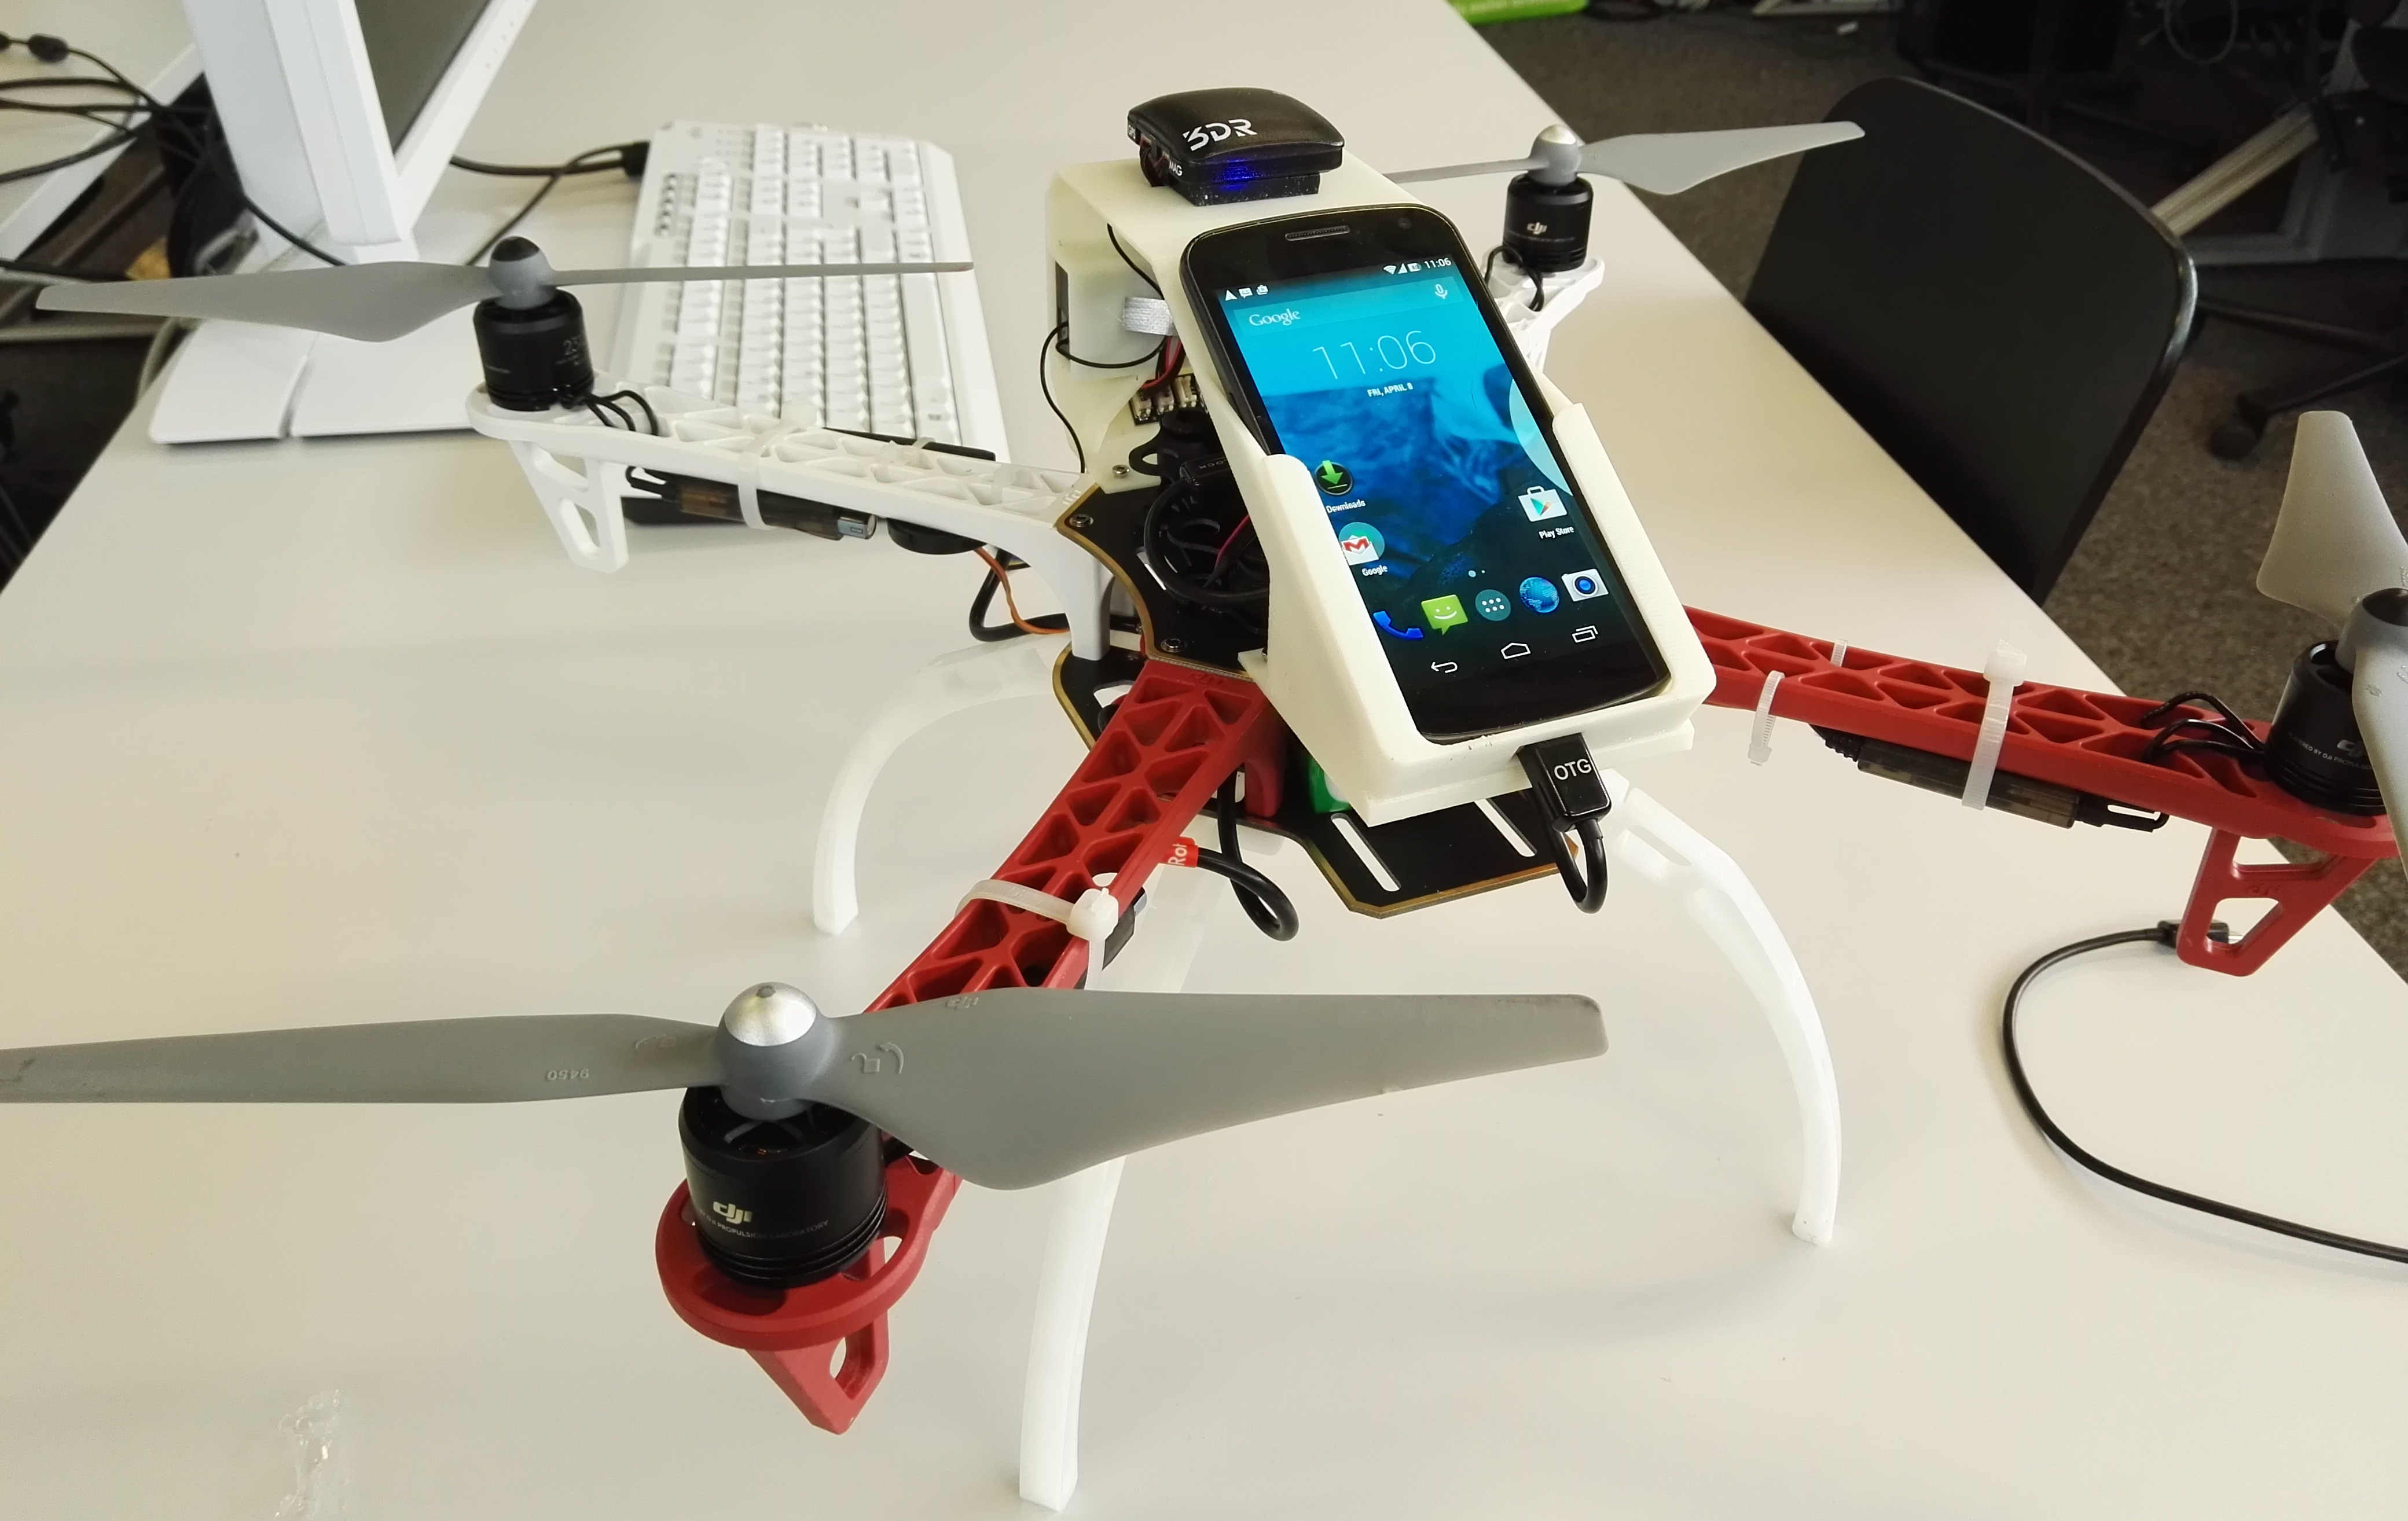
\includegraphics[width=\textwidth]{images/hardware/drone-with-handy.jpg}
	\caption{Drohne mit Handy Halterung}
	\label{fig:prototyp-3}
	\end{minipage}
	\hfill
	\begin{minipage}[b]{0.4\textwidth}
		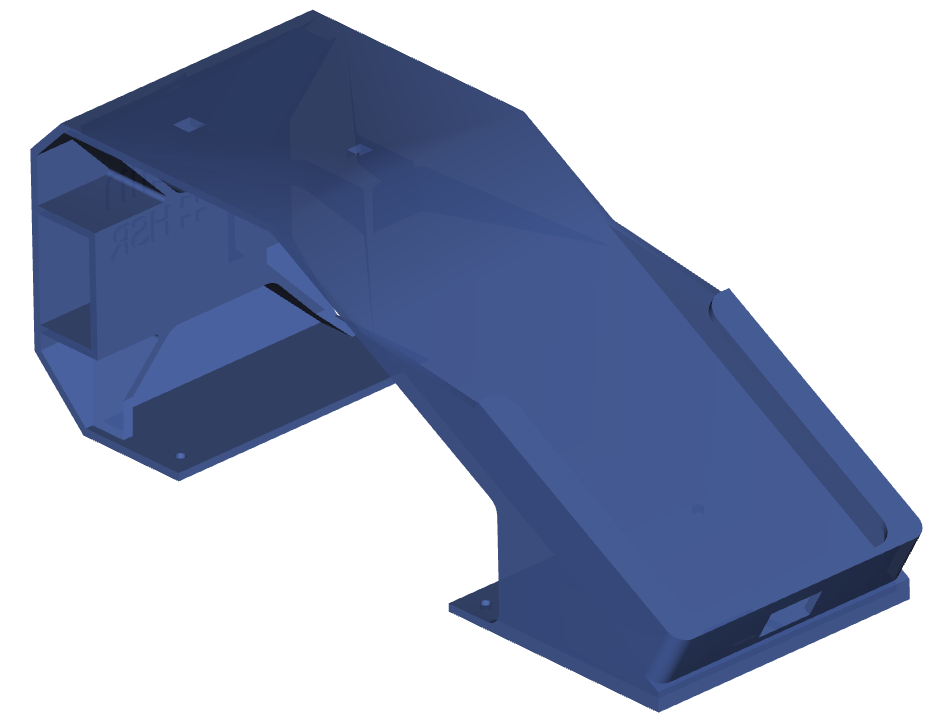
\includegraphics[width=\textwidth]{images/hardware/case-model.png}
	\caption{3D-Modell der Handy Halterung}
	\label{fig:case-model}
	\end{minipage}
\end{figure}

Es wurde eine Halterung konzipiert (siehe Abb.\ref{fig:case-model}), welche wir im 3D-Druck Verfahren produzieren liessen.
Die Handy-Halterung konnte auch gleich genutzt werden, um das GPS-Modul an einer passenden Stelle zu positionieren. 

\subsubsection{Version 3}
Nachdem mit der Drohne zahlreiche autonome Testflüge unternommen wurden, musste eine Möglichkeit erarbeitet werden, wie die Lieferung an den Kunden gebracht werden kann.

\begin{figure}[H]
	\centering
	\begin{minipage}[b]{0.4\textwidth}
		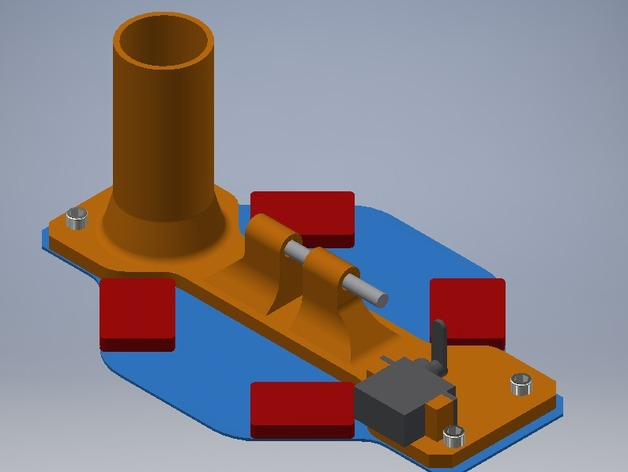
\includegraphics[width=\textwidth]{images/hardware/parachute-model.jpg}
		\caption{Halterung}
		\label{fig:parachute-mode}
	\end{minipage}
	\hfill
	\begin{minipage}[b]{0.4\textwidth}
		% TODO Hier muss ein bessers Bild her ( oder Kafferahmen weg photoshoppen )
		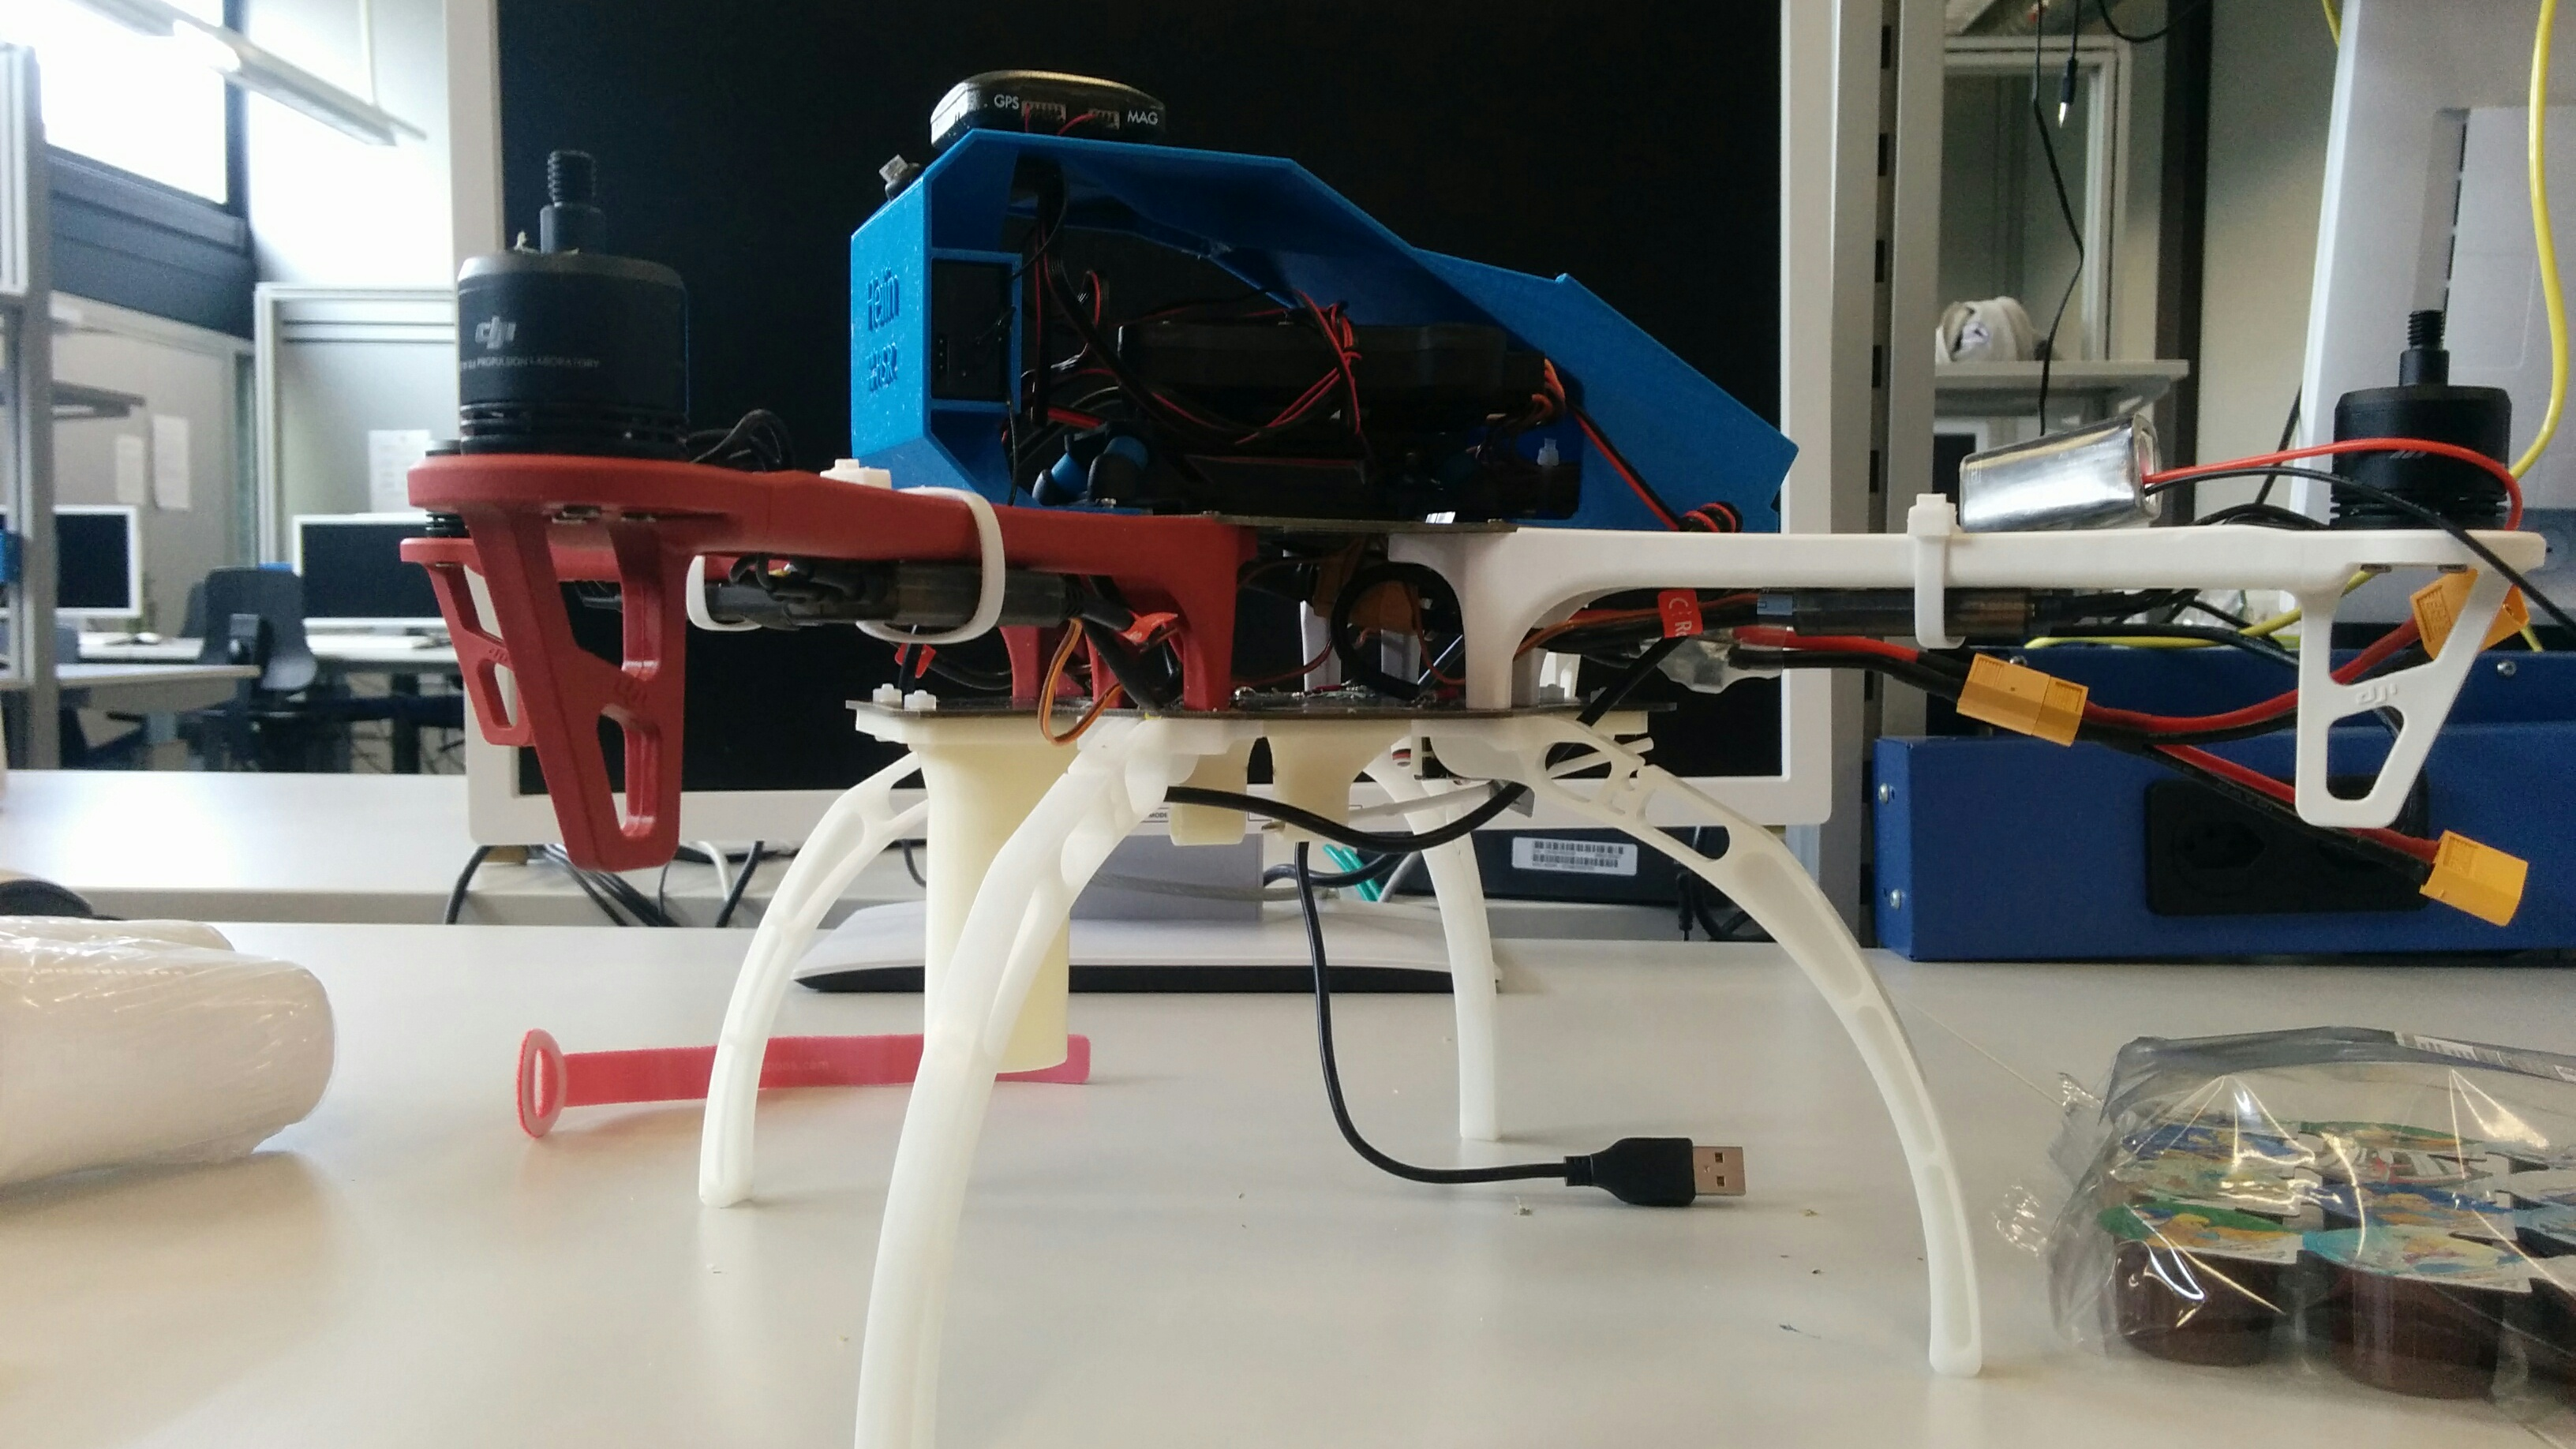
\includegraphics[width=\textwidth]{images/hardware/drone-with-servo.jpg}
		\caption{Drohne mit dem Abwurfsmechanismus}
		\label{fig:drone-with-servo}
	\end{minipage}
\end{figure}


Es wurde ein einfacher Mechanismus mit einem handelsüblichen Modelbau-Servo konstruiert. Die Abbildung \ref{fig:drone-with-servo} zeigt, den Mechanismus mit dem Stift, der vom Servo herausgezogen werden kann. Das Rohr auf der Vorrichtung dient zur Aufbewahrung des Fallschirms während des Flugs. Nach dem Lösen des Stifts zieht das Gewicht der Ladung den Fallschirm aus dem Rohr.\\

\subsection{Kommunikationshardware}
\label{sec:communication-hardware}
=======
\section{Kommunikationshardware}
>>>>>>> 9bc3b404e6fc6214d2424b8a17ca7f0adf126991
Da die Drohne eine Verbindung zum Server benötigt, muss geeignete Kommunikationshardware installiert werden. Aus folgenden Gründen haben wir uns für ein Android-Smartphone entschieden:
\begin{itemize}
	\item{Der Status der Drohne und Anweisungen zur Beladung können angezeigt werden}
	\item{Die Anbindung an den Flight-Controller ist über eine bestehende API möglich}
	\item{Das Android-Betriebssystem stellt die Kommunikation über WLAN oder GSM zur Verfügung}
\end{itemize}

Falls die Beladung automatisiert wird, oder keine Beladung notwendig ist, benötigt man nicht zwingend ein Smartphone. Um Gewicht und Platz auf der Drohne zu sparen gibt es folgende Alternativen:
\begin{itemize}
	\item{\textbf{Raspberry PI} \\
	Bereits ab dem leichtgewichtigen Raspberry PI zero sind die nötigen Funktionen vorhanden. Zusätzlich muss hier auf ein GSM Modem zurückgegriffen werden um eine permanente Internetverbindung aufzubauen. Bei Verwendung eines Raspberry PI 3 kann sogar auf ein eingebautes WLAN Interface verwendet werden.
	}
	\item{\textbf{Arduino} \\
	Bei der Arduino Hardware Plattform kann auf einem beliebigen Arduino Board implementiert werden, welches als USB Host Device arbeiten kann. Zusätzlich muss ein GSM Shield 2 verwendet werden um eine GSM Verbindung aufbauen zu können. Eine Option auf WLAN existiert nur durch zusätzliche Komponenten.}
	\item{\textbf{Pixhawk Controller mit GSM Modul} \\
	Es existieren GSM Module, wie etwa DroneCell \ref{drone-cell}, um am Pixhawk anzuschliessen. Diese werden aber dazu genutzt um Telemetriedaten zu übertragen. Da die verwendete Firmware für Pixhawk opensource ist, besteht die Möglichkeit die Firmware anzupassen, um bidirektionale Kommunikation über das GSM Module zu ermöglichen.
	}

\end{itemize}

Die ersten zwei Alternativen bringen zusätzlich mit sich, dass sie externe Stromversorgung benötigen. Somit muss, um eine stabile Betriebsspannung zu generieren, auf die Bordstromversorgung zurückgegriffen werden und ein \Gls{BEC}, welches für eine konstante Spannung sorgt, für die Servo-Stromversorgung verwendet werden. \\

Abschliessend kann gesagt werden, dass das von uns verwendete Smartphone (Nexus 4) 139 Gramm schwer ist. Die Lösung mit dem Raspberry PI 3 schlägt mit 40 Gramm zu buche. Die Einsparung von 100 Gramm bringt einen Verzicht auf ein Display und den Zwang einer zusätzlichen Stromversorgung mit sich.


\section{Ablieferungskonzept}
\label{chap:ablieferung}
Um ein möglichst sicheres und einfaches Ablieferungsverfahren zu finden, wurden folgende Optionen in Betracht gezogen.

\subsection{Landung ohne automatischen Abwurf}

Bei diesem Konzept landet die Drohne an der Position des Kunden und dieser kann dann selbst das Paket von der Drohne lösen. Er wird dann mit Hilfe der Onboard-App aufgefordert den Erhalt der Bestellung zu bestätigen. Nach der Bestätigung startet die Drohne einen Countdown, hebt danach ab und fliegt zur Ausgangsposition zurück. Der Kunde kann den Countdown unterbrechen und erneut starten.

Vorteile:
\begin{itemize}
	\item Kunde bestätigt Lieferung
	\item Ware kann keinen Schaden nehmen
	\item Kunde kann entscheiden wann es sicher genug ist, damit die Drohne starten kann.
	\item Die Lieferung ist punktgenau 
\end{itemize}


Nachteile:
\begin{itemize}
	\item Drohne kann Personen verletzen, während sie sich in Bodennähe befindet
	\item Aufwendiges Handling auf der Onboard-App
	\item Landung kann je nach Gelände schwierig sein 
	\item Fremde Personen haben physischen Zugriff auf die Drohne
\end{itemize}

\subsection{Landung mit automatischem Abwurf}

Dieses System ermöglicht es ohne Fallschirm die Ware abzuwerfen. Dabei Landet die Drohne, löst die Ladung und startet sofort wieder. Es gibt keinerlei Interaktion mit dem Kunden.

Vorteile:
\begin{itemize}
	\item Ware kann keinen Schaden nehmen
\end{itemize}


Nachteile:
\begin{itemize}
	\item Drohne kann Personen verletzen, während sie sich in Bodennähe befindet
	\item Landung kann schwierig sein je nach Gelände
	\item Fremde Personen haben physischen Zugriff auf die Drohne
\end{itemize}


\subsection{Abwurf mit Fallschirm}

Dabei wird ein Fallschirm an der Ware befestigt. Die Drohne löst die Ladung in einer vorgegebenen Höhe und die Ladung schwebt zu Boden.

Vorteile:
\begin{itemize}
	\item Drohne kann niemanden Verletzen 
	\item Drohne ist ausser Reichweite von Personen
	\item Einfaches Handling auf der Onboard-App
	\item Mechanismus erlaubt auch Landung mit automatischem Abwurf
\end{itemize}


Nachteile:
\begin{itemize}
	\item Ware kann Schaden nehmen
	\item Ware kann Personen verletzen bei Versagen des Fallschirms
	\item Einweg Fallschirme (Kosten und Abfall)
	\item Windlage kann Fallschirm Flugrichtung beeinflussen
\end{itemize}


\subsection{Entscheidung}

\begin{figure}[H]
	\centering
	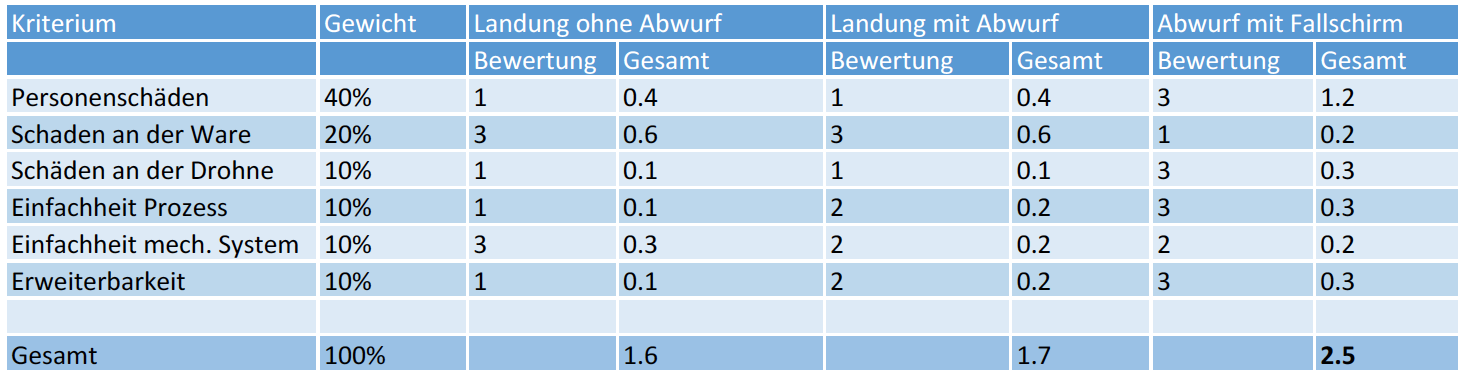
\includegraphics[width=0.9\textwidth] {images/nutzwertanalyse_abwurf.png} 
	\caption{Nutzwertanalyse der verschiedenen Liefervarianten}
	\label{fig:nutzwertanalyse_abwurf}
\end{figure}


Die Nutzwertanalyse in Abbildung \ref{fig:nutzwertanalyse_abwurf} zeigt klar, dass die letzte Variante die meisten Vorteile bringt. Wichtig ist auch, dass ein Abwurf im gelandeten Zustand weiterhin möglich bleibt, ohne die mechanischen Komponenten zu verändern. Deshalb haben wir uns für einen Abwurf mit dem Fallschirm entschieden.

\subsection{Fallschirmgrösse}

Für den Fallschirm musste die optimale Grösse berechnet werden. Aufgrund der Resultate aus dem Tragfähigkeitstests wird die Grösse für eine $1/2$-Liter Flasche berechnet.
Eine PET-Flasche die von einem ein Meter hohen Tisch fällt, bleibt unbeschädigt. Aus diesem Grund haben wir die Geschwindigkeit für diesen Aufprall errechnet.

\begin{equation}
\label{eq:pet}
\begin{split}
v &= \sqrt{2gd} \\
v &= \sqrt{2 \cdot 9.81\frac{\text{m}}{\text{s}^2} \cdot 1.0\text{m}} \\
v &= 4.429 \frac{\text{m}}{\text{s}} \approx 4.5 \frac{\text{m}}{\text{s}} \\
\end{split}
\end{equation}

Nun musste der Fallschirm dimensioniert werden. 
Einfachheitshalber wird angenommen, dass der Fallschirm die Form einer Kugelkalotte hat und ein Zielgewicht von 500g. Die Fläche des Fallschirms kann anhand der folgender Gleichung ausgedrückt werden:


%Todo Skizze
\begin{equation}
\begin{split}
F_{Brems} &= F_{G} \\
c_{w} \cdot A \cdot \frac{\rho}{2} \cdot v_{sink}^{2} &= m_{Pet} \cdot g \\
A &= \frac{2 \cdot m_{Pet} \cdot g}{\rho \cdot c_{w} \cdot v_{sink}^{2} } \\
\end{split}
\end{equation}

Nun lässt sich der Durchmesser ($d$) über die Öffnungsfläche $A = \pi \cdot r^2$ berechnen. Wir näheren an, dass der Öffnungsdurchmesser dem Fallschirmdurchmesser entspricht. 

\begin{equation}
\begin{split}
\pi \cdot r^2 &= \frac{2 \cdot m_{Pet} \cdot g}{\rho \cdot c_{w} \cdot v_{sink}^{2} } \\
r &= \sqrt{\frac{2 \cdot m_{Pet} \cdot g}{\rho \cdot c_{w} \cdot v_{sink}^{2} \cdot \pi}} \\
d &= 2 \cdot \sqrt{\frac{2 \cdot m_{Pet} \cdot g}{\rho \cdot c_{w} \cdot v_{sink}^{2} \cdot \pi}} \\
\end{split}
\end{equation}

Für die Werte $\rho$, $c_w$ wurden die Standardwerte genommen. Bei der Luftdichte $\rho$ entspricht das $1.225 \frac{kg}{m^3}$. 
Für den Strömungswiderstandskoeffizenten $c_w$ wird der Literaturwert für die konkave Seite der Halbkugelschale $1.33$ eingesetzt. Herr Prof. Dr. F. Müller hat uns darauf hingewiesen, dass bei seinen Raketenversuche, er einen $c_w$-Wert von 1.8 als gute Annäherung verwendet. Aus diesem Grund haben wir diesen für die weitere Berechnung eingesetzt.
\begin{equation}
\begin{split}
d &= 2 \cdot \sqrt{\frac{2 \cdot 0.5\text{kg} \cdot  9.81\frac{\text{m}}{\text{s}^2}}{1.225 \frac{\text{kg}}{\text{m}^3} \cdot 1.80 \cdot 4.5 \frac{\text{m}}{\text{s}} \cdot \pi}} \\
d &= 1.12\text{m} \\
\end{split}
\end{equation}
Der Durchmesser des Prototypenfallschirms muss somit etwa 1.12m betragen.

\newpage
\section{Multicopter Hardware}

Bei der Zusammenstellung der Komponenten haben wir vor allem auf die gute Verfügbarkeit von 
Ersatzteilen und einen hohen Marktanteil der Komponenten geachtet. Besonders wichtig erschien uns, dass ein Anbieter nicht an einen Hersteller gebunden ist, sondern die Drohne an seine Bedürfnisse (Zuladung, Reichweite, Geschwindigkeit) anpassen kann. Es sollten also möglichst wenige Voraussetzungen bestehen um die Plattform nutzen zu können. Folgende Anforderungen sind allerdings unabdingbar:
\begin{itemize}
	\item Flight-Controller muss \Gls{MAVLink} Protokoll unterstüzen
	\item Onboard-App muss über MAVLink mit dem Flight-Controller verbunden sein. (Über USB oder eine Funk-Telemetrieverbindung.)
\end{itemize}

\subsection{Teile-Liste}

\begin{tabularx}{\textwidth}{|X|l|l r|}
	\hline
	\textbf{Bezeichnung} & \textbf{Bezugsquelle} && \textbf{Preis}\\
	\hline \hline
	DJI F450 ARF Kit & conrad.ch & CHF &229.95 \\\hline
	DJI F450/F550 Landegestell & conrad.ch & CHF &24.95 \\\hline
	3DR Pixhawk & 3dr.com & USD& 199.99 \\\hline
	3DR uBlox GPS with Compass Kit & 3dr.com & USD &89.99 \\\hline
	Pixhawk external LED and USB & 3dr.com & USD & 20.00 \\\hline
	FrSky X8+ Radio Transmitter & 3dr.com & USD & 89.99 \\\hline
	FrSky X8R Receiver & hebu-shop.ch & CHF & 39.95 \\\hline
	Delock Micro USB OTG Kabel & digitec.ch & CHF &15.90 \\\hline
	Multistar High Capacity 4S Akku (2x) & hobbyking.com & USD& 50.50 \\\hline
	APM Flight Controller Damping Platform & hobbyking.com & USD& 2.69 \\\hline
	Smartphone und GPS Halterung & eigener 3D-Print & CHF &27.50\\\hline
	Abwurfvorrichtung & eigener 3D-Print & CHF &25.50\\\hline
	Hitec Super Servo S-Bec (Stromversorgung Servo) & brack.ch & CHF &13.90\\\hline
	Tactic TSX10 (Servo für Abwurf) & brack.ch & CHF & 14.90\\\hline
	Kleinmaterial & diverse & CHF & 50.00\\\hline
	\hline
	\textbf{Total} & & \textbf{CHF/USD} & $\boldsymbol{\approx 900.00}$\\\hline
\end{tabularx}

\subsection{Frame und Antrieb}

Der Frame, die Motoren und ESCs wurden als Kit gekauft. Es handelt sich dabei um ein DJI Flamewheel 450 Frame mit DJI 2312 960kV Motoren und ESeries 420 20A ESCs. Dieses Kit ist weltweit gut verfügbar und deshalb ideal geeignet um einen Versuchsaufbau zu erstellen.

\begin{figure}[h]
	\centering
	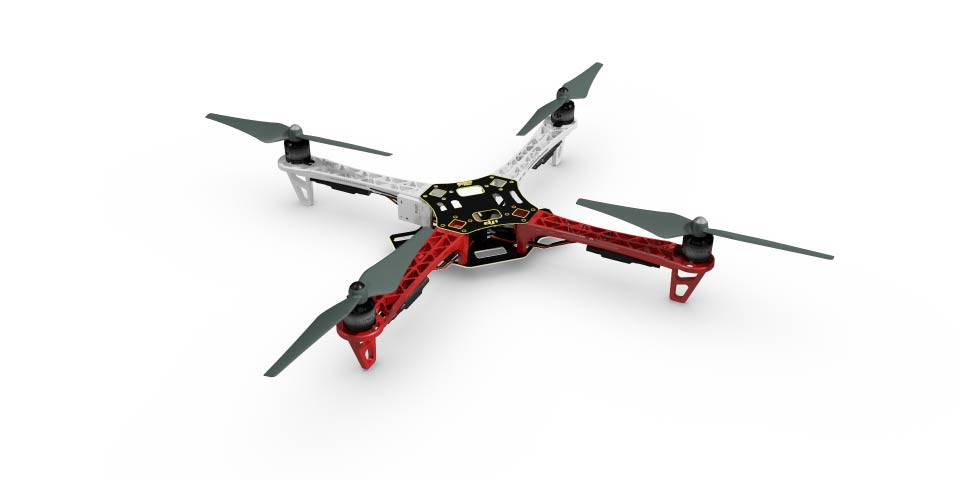
\includegraphics[width=0.9\textwidth] {images/hardware/f450.jpg} 
	\caption{DJI F450 Flamewheel Kit}
	\label{fig:f450}
\end{figure}


\subsection{Flight-Controller}

Der Flight-Controller ist das Herzstück eines Multicopters. Im Unterschied zu anderen ferngesteuerten Fahr- und Flugzeugen kann ein Multicopter nur über ein Fly-by-Wire System kontrolliert werden. Das heisst alle Befehle, die von der Fernbedienung gesendet werden, müssen interpretiert und umgewandelt werden, damit die Motoren eine Bewegung in die gewünschte Richtung erzeugen können. In Kombination mit einem GPS Modul (Abb. \ref{fig:gps-module}) ermöglich der Controller verschiedene Flugmodi, wie beispielsweise das Schweben an einem Punkt oder automatisches Abfliegen von Wegpunkten.

Als Flight-Controller setzen wir ein Pixhawk ein. Es ist sehr vielseitig und kann gut mit zusätzlichen Sensoren erweitert werden, ausserdem unterstützt es gängige Firmwares, die auch auf günstigeren Controllern laufen. Als Firmware für das Pixhawk setzen wir ArduCopter ein, da sie komplett Open-Source ist und auch bei vielen anderen Projekten eingesetzt wird. Sie unterstützt ausserdem das \Gls{MAVLink} Protokoll.

\begin{figure}[h]
	\centering
	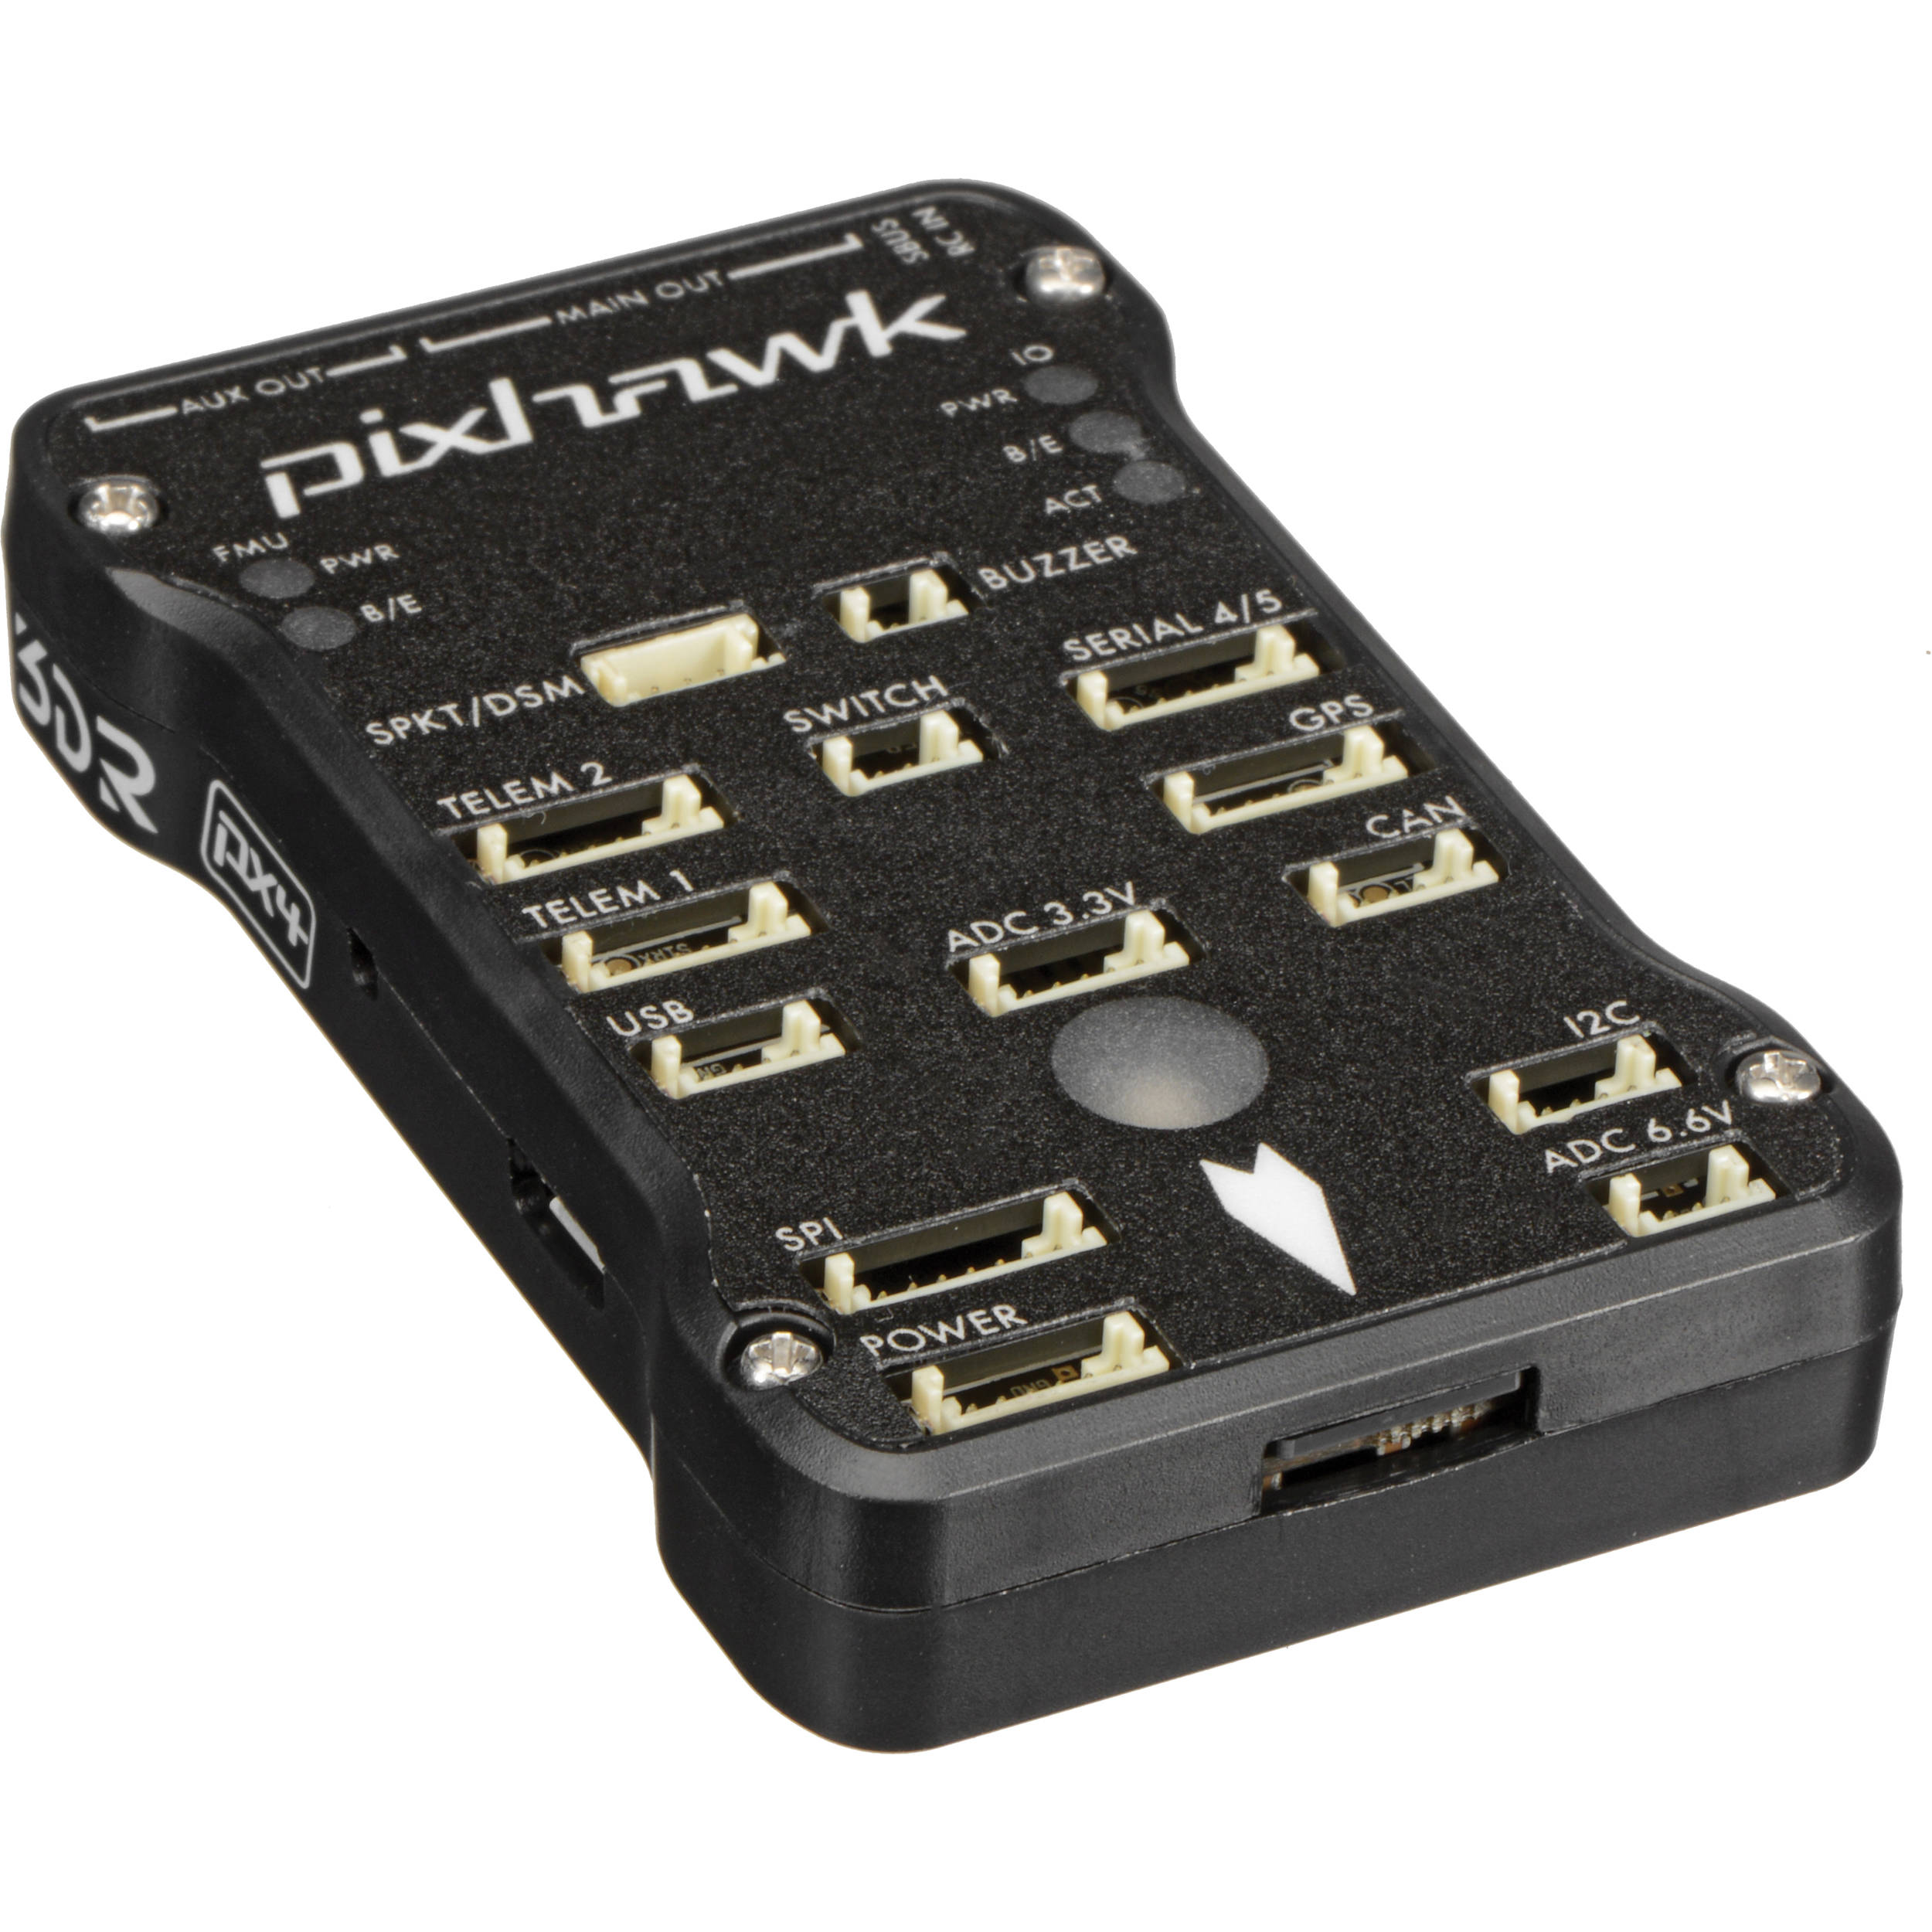
\includegraphics[width=0.3\textwidth] {images/hardware/pixhawk.jpg} 
	\caption{Pixhawk Flight-Controller}
	\label{fig:pixhawk}
\end{figure}

\begin{figure}[h]
	\centering
	
\includegraphics[width=0.3\textwidth] {images/hardware/gps-module.jpg} 
	\caption{GPS-Modul für Pixhawk}
	\label{fig:gps-module}
\end{figure}

\subsection{Ausbaustufen}

Während des Projekts wurde die Hardware laufend den Bedürfnissen angepasst. Daher sind mehrere Versionen der Drohne entstanden, die für die Versuche genutzt wurden und geholfen haben Risiken früh auszuschliessen.

\subsubsection{Version 1}

\begin{figure}[H]
	\centering
	\includegraphics[width=0.4\textwidth] {images/hardware/prototype1.jpg}
	\caption{Erster Prototyp ohne Landegestell und ohne Smartphone}
	\label{fig:prototyp-1}
\end{figure}

Um das Zusammenspiel der Hardwarekomponenten zu testen und erste Erfahrungen mit dem GPS und den verschiedenen Flugmodi zu sammeln, wurde in der ersten Iteration nur die Drohne in einem minimal Flugzustand aufgebaut.

\subsubsection{Version 2}

\begin{figure}[H]
	\centering
	\includegraphics[width=0.4\textwidth] {images/hardware/prototype2.jpg}
	\caption{Drohnen Aufbau mit Smartphone}
	\label{fig:prototyp-2}
\end{figure}

Um die Risiken R08 (Ardupilot Handhabung) und R09 (Ardupilot API) frühzeitig auszuschliessen (siehe Tabelle \ref{table:risk-table}), wurde das Smartphone provisorisch auf die Drohne montiert, und mit einem ersten Prototypen der Onboard-App getestet. \\
Nach dem Test wurde uns klar, dass eine Befestigung für das Smartphone erarbeitet werden musste, um es sicher zu transportieren und bedienbar zu positionieren.

\begin{figure}[H]
	\centering
	\begin{minipage}[b]{0.4\textwidth}
		% TODO Ein Bild ohne Tastatur und Stuhl wäre auch gut?
		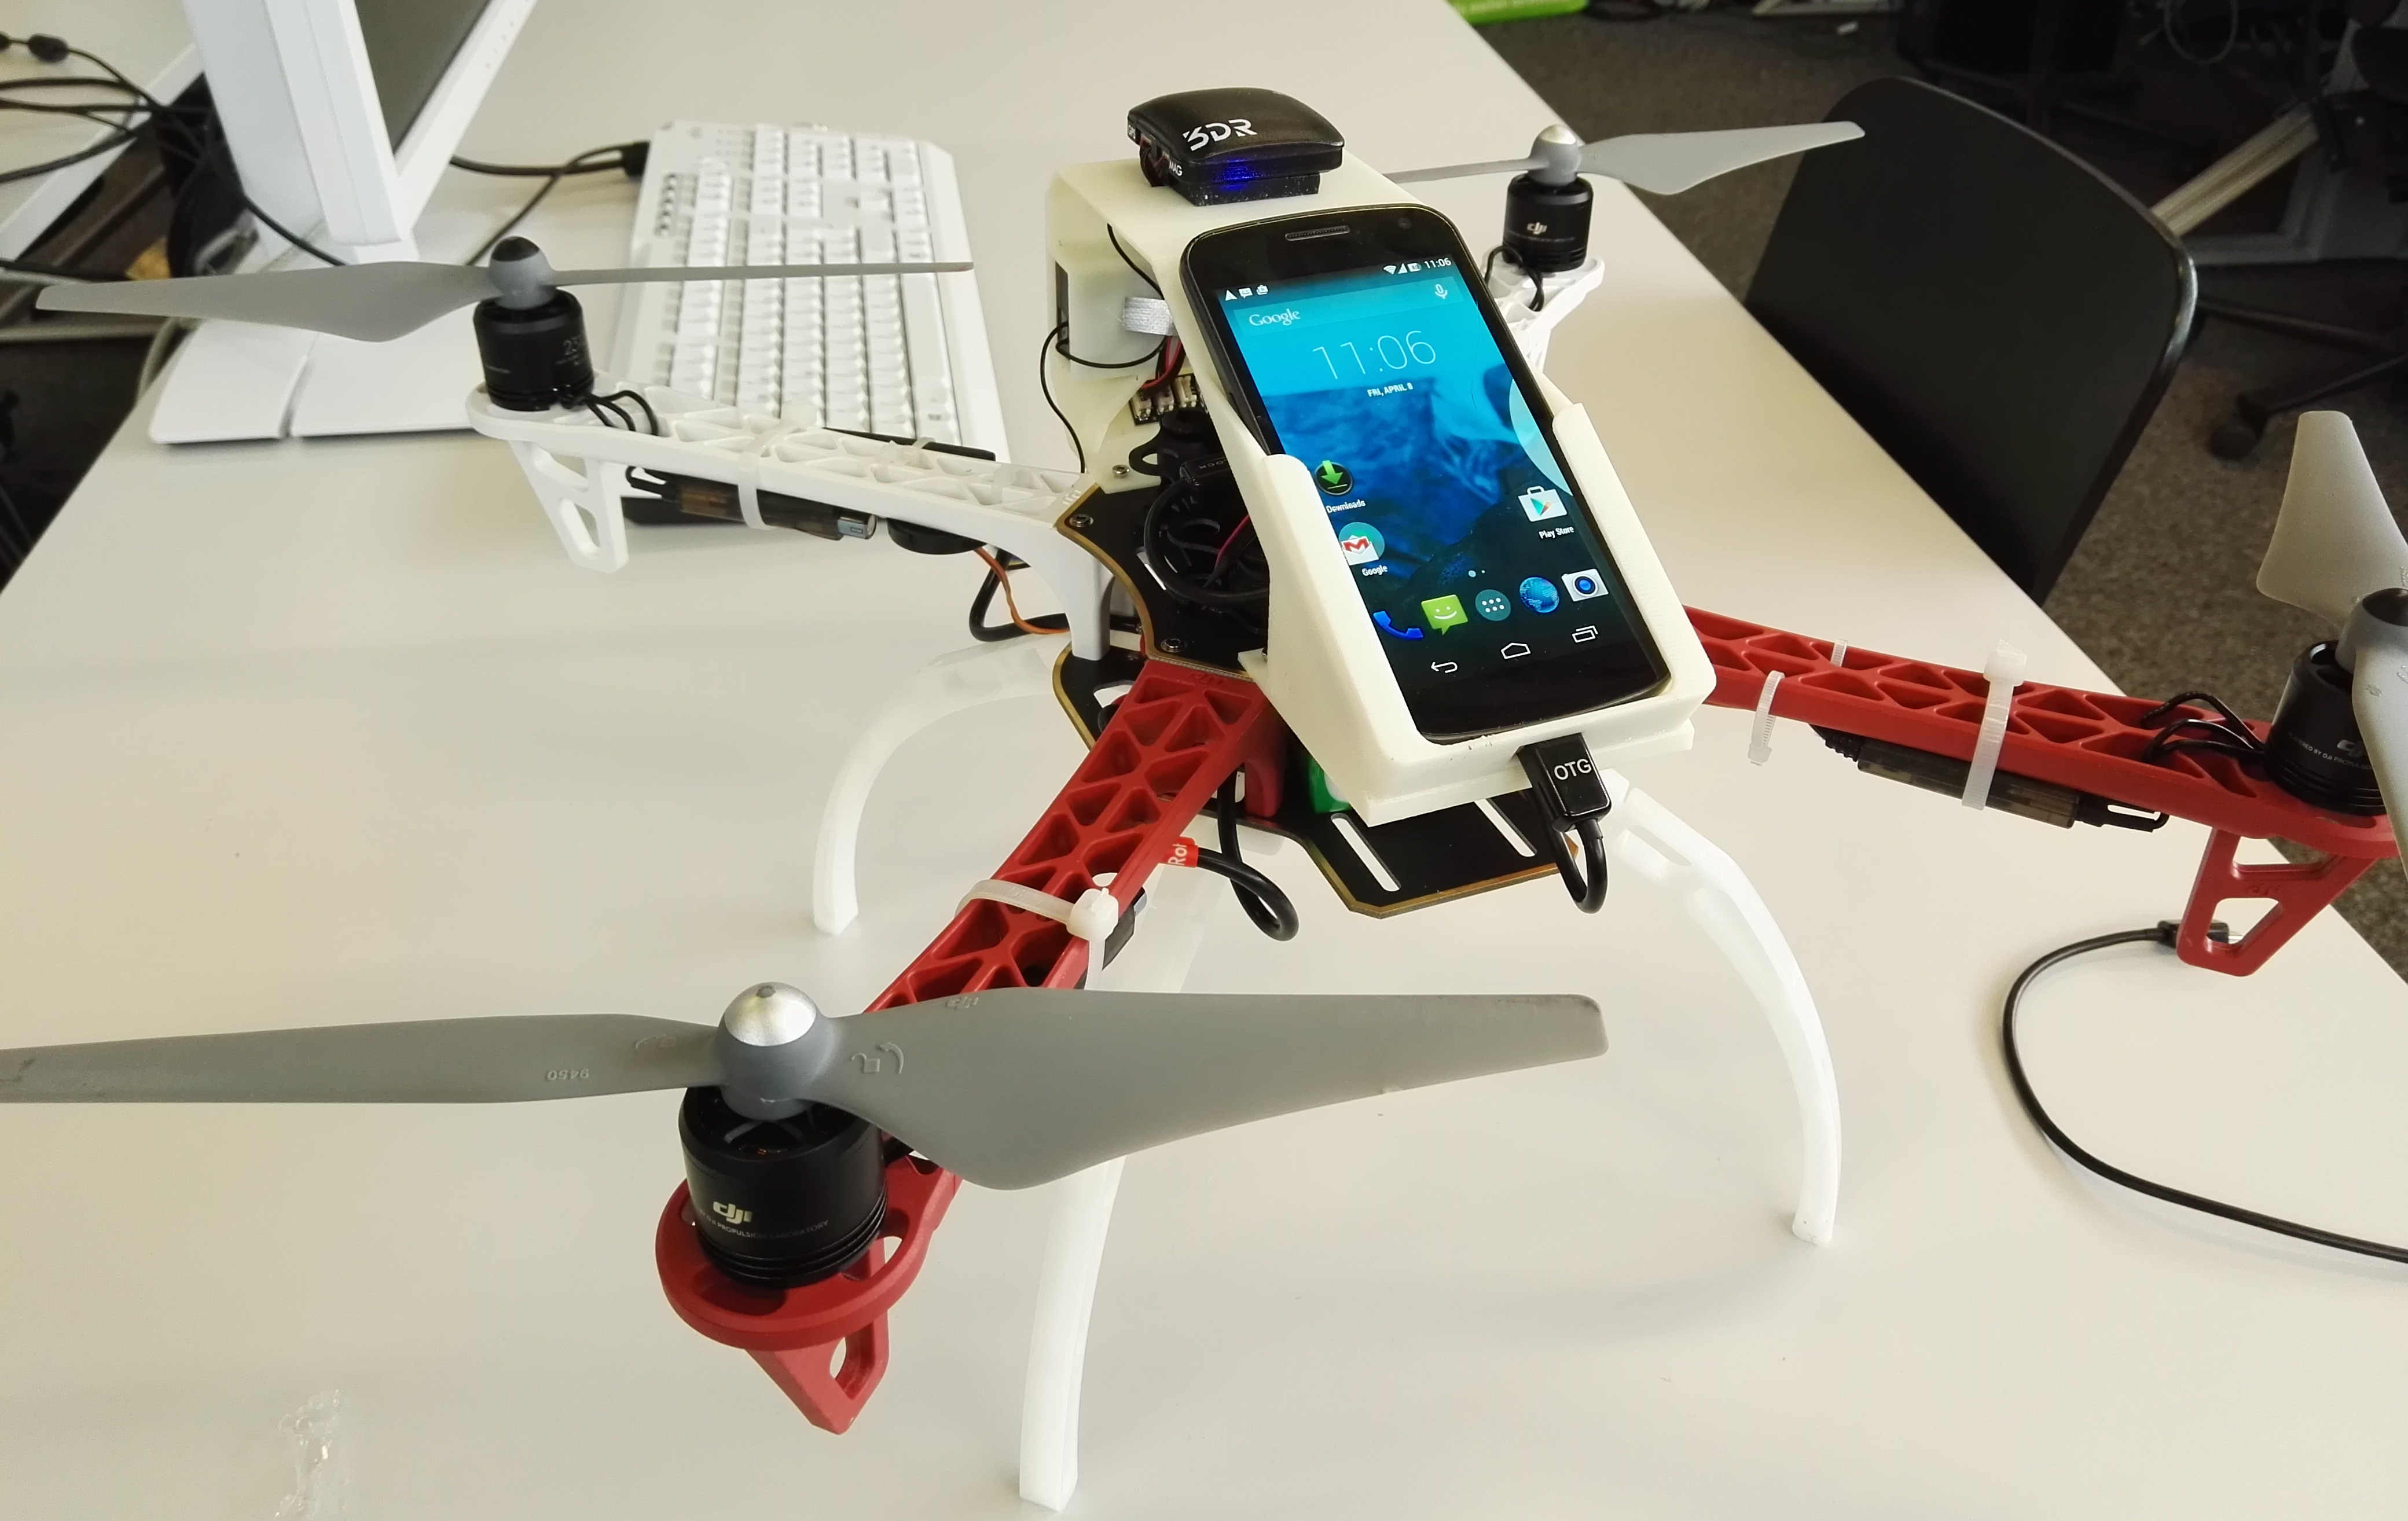
\includegraphics[width=\textwidth]{images/hardware/drone-with-handy.jpg}
		\caption{Drohne mit Handy Halterung}
		\label{fig:prototyp-3}
	\end{minipage}
	\hfill
	\begin{minipage}[b]{0.4\textwidth}
		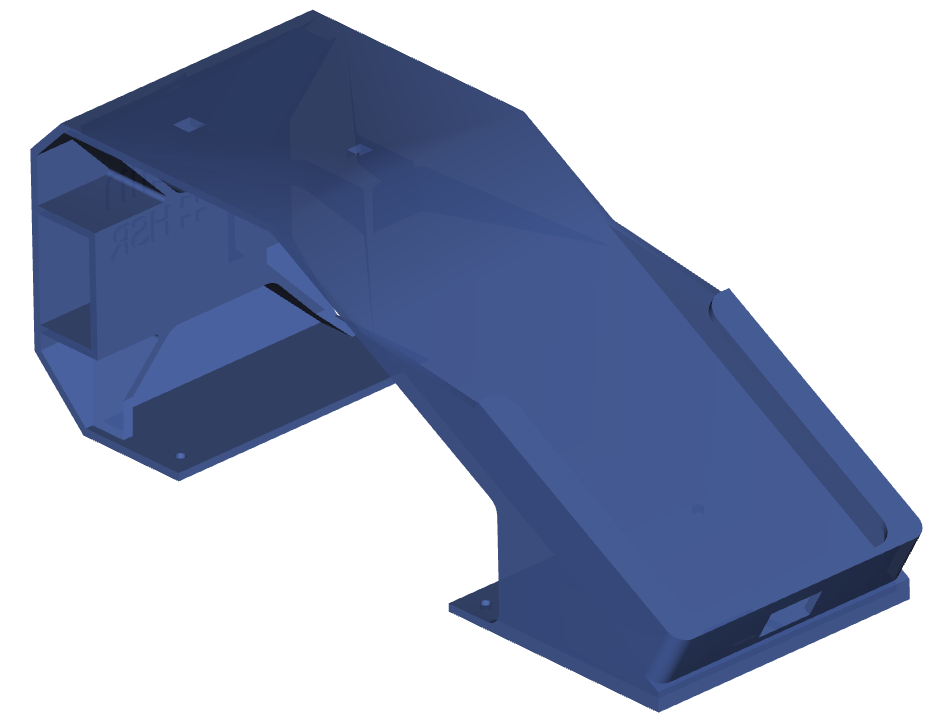
\includegraphics[width=\textwidth]{images/hardware/case-model.png}
		\caption{3D-Modell der Handy Halterung}
		\label{fig:case-model}
	\end{minipage}
\end{figure}

Es wurde eine Halterung konzipiert (siehe Abb.\ref{fig:case-model}), welche wir im 3D-Druck Verfahren produzieren liessen.
Die Handy-Halterung konnte auch gleich genutzt werden, um das GPS-Modul an einer passenden Stelle zu positionieren. 

\subsubsection{Version 3}
Nachdem mit der Drohne zahlreiche autonome Testflüge unternommen wurden, musste eine Möglichkeit erarbeitet werden, wie die Lieferung an den Kunden gebracht werden kann ( Abschnitt \ref{chap:ablieferung} ).

\begin{figure}[H]
	\centering
	\begin{minipage}[b]{0.4\textwidth}
		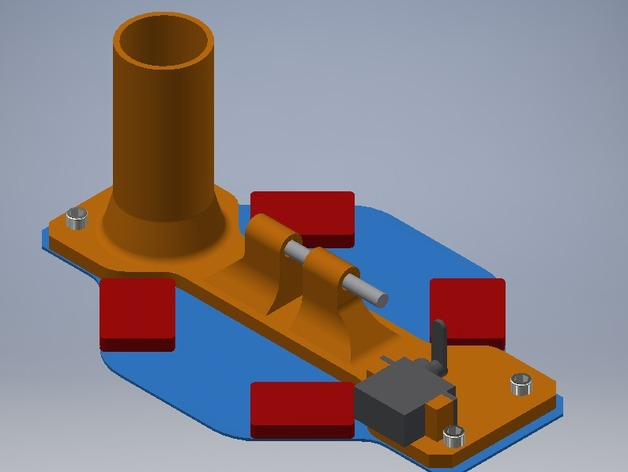
\includegraphics[width=\textwidth]{images/hardware/parachute-model.jpg}
		\caption{Halterung}
		\label{fig:parachute-mode}
	\end{minipage}
	\hfill
	\begin{minipage}[b]{0.4\textwidth}
		% TODO Hier muss ein bessers Bild her ( oder Kafferahmen weg photoshoppen )
		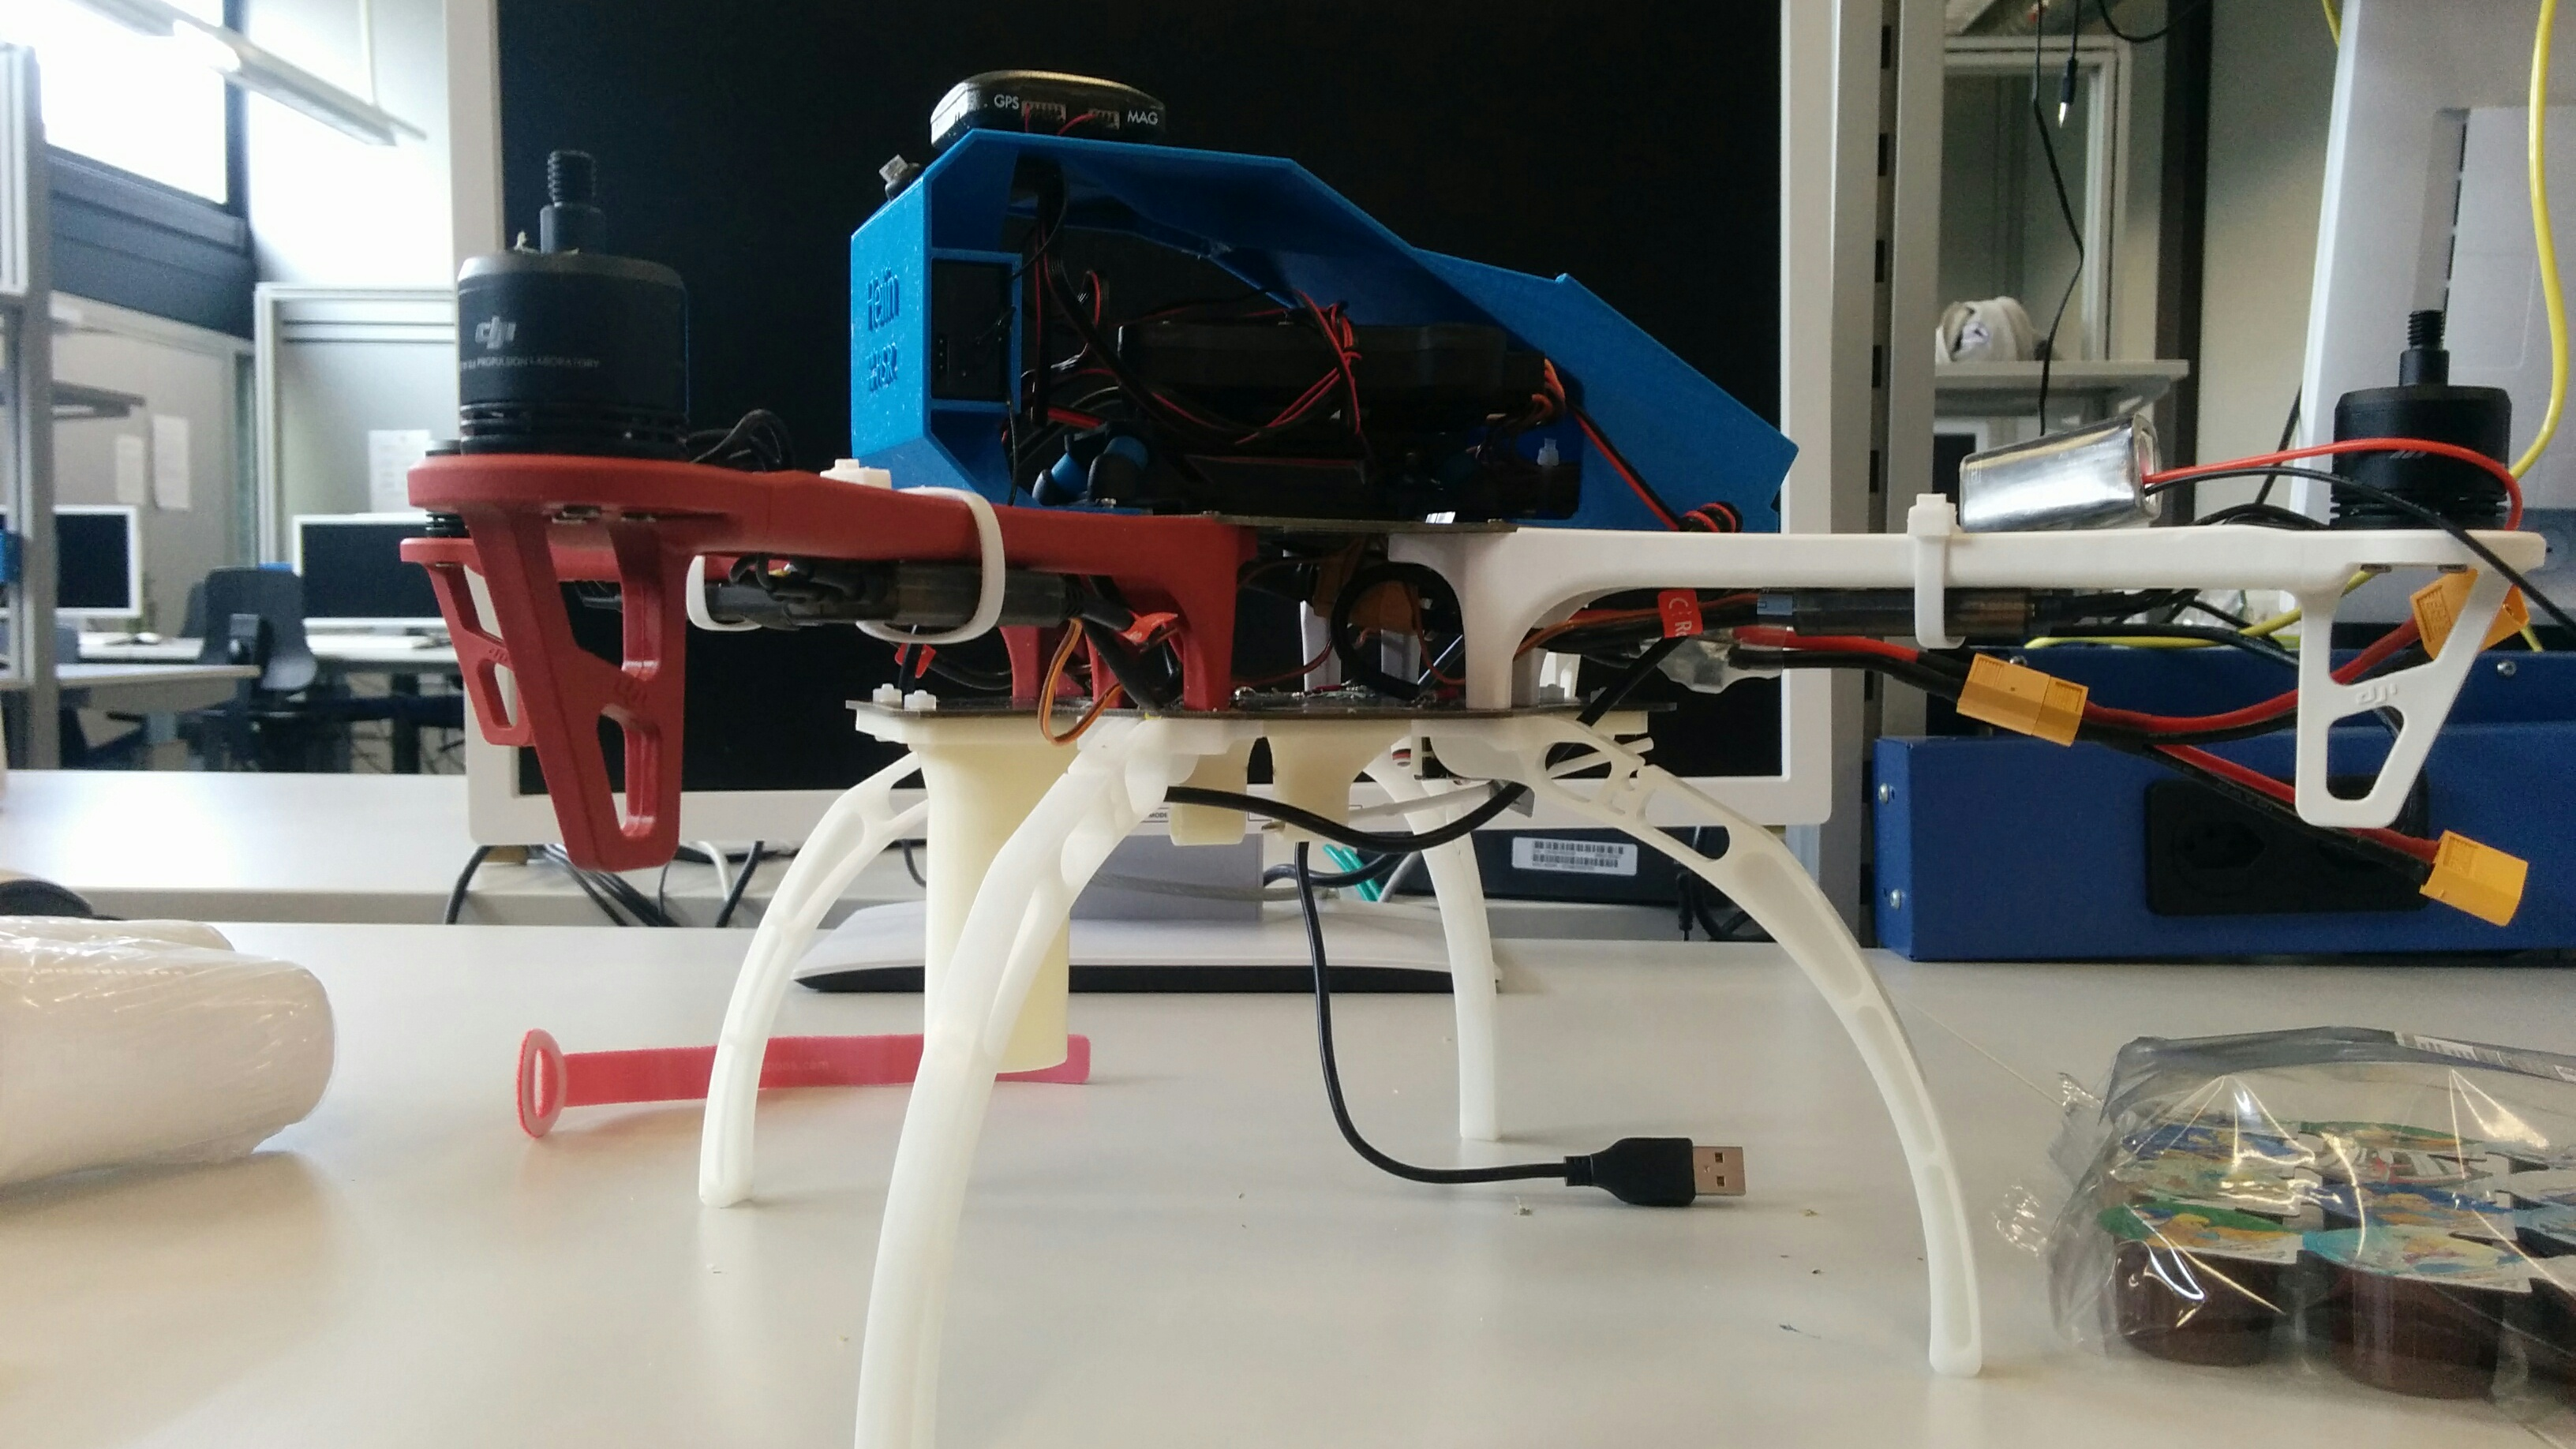
\includegraphics[width=\textwidth]{images/hardware/drone-with-servo.jpg}
		\caption{Drohne mit dem Abwurfsmechanismus}
		\label{fig:drone-with-servo}
	\end{minipage}
\end{figure}


Es wurde ein einfacher Mechanismus mit einem handelsüblichen Modelbau-Servo konstruiert. Die Abbildung \ref{fig:drone-with-servo} zeigt, den Mechanismus mit dem Stift, der vom Servo herausgezogen werden kann. Das Rohr auf der Vorrichtung dient zur Aufbewahrung des Fallschirms während des Flugs. Nach dem Lösen des Stifts zieht das Gewicht der Ladung den Fallschirm aus dem Rohr.\\

\subsection{Tests}
Um die Anwendungsmöglichkeiten eines solchen Multicopters auszuloten wurden diverse Experimente durchgeführt um die Leistungsfähigkeit und die Einschränkungen zu testen. 

\subsubsection{Akku Laufzeittest}
Um die maximale Akku Laufzeit zu testen wurde die Drohne ohne zusätzliches Gewicht gestartet, etwa 1.5m über dem Boden schweben gelassen und die Zeit gemessen. Dabei versucht die Drohne die Postion zu halten, bei Abweichung wurde aktiv korrigiert. \\

\begin{tabularx}{\textwidth}{|c|c|X|}
	\hline
	\textbf{Akku} & \textbf{Zuladung} & \textbf{Laufzeit} \\ \hline \hline 
	3S & keine & 16min 29s\\ \hline 
	2x 4S & 500g & 19min\\ \hline 
\end{tabularx}

\subsubsection{Tragfähigkeitstests}
Um das maximale Gewicht zu prüfen, welches auf unsere Drohnen geladen werden kann, wurden Tests mit dem Zielgewicht von ca. 500g durchgeführt. Dies Entspricht dem Gewicht einer $1/2$-Liter Flasche oder einem leichten Defibrilator. Ausserdem war das Mobiltelefon (ca. 150g) während des Tests auf der Drohne angebracht.  \\

\begin{tabularx}{\textwidth}{|c|c|c|c|X|}
	\hline
	\textbf{Nutzlast} & \textbf{Akku Typ} & \textbf{Nötige Leistung }& \textbf{Erwartete Flugzeit } & \textbf{Subjektives Flugverhalten }\\
	\hline \hline
	500g & 3S & ca. 75\%  & n.A. & Ziemlich Träge, mehr Gewicht wäre kritisch\\\hline
	500g & 4S & ca. 45\%  & n.A. & Gewicht kaum Spürbar\\
	\hline
\end{tabularx}\\

Auch mit 3S Akkus ist es also möglich eine PET-Flasche zu transportieren. Allerdings empfehlen wir für Gewichte über 300 Gramm 4S-Akkus zu verwenden.\\

Aus den Tragfähigkeitstests schliessen wir, dass auch ein Defibrillator (siehe Aufgabenstellung) mit einer von uns erstellten Drohne transportierbar ist. Folgende Textpassage \cite[p.3]{FleckUAV} bestätigt, dass in einem ähnlichen Gewichtsbereich bereits Produkte existieren.

\blockquote{I identified the two lightest weight defibrillators on the market in the U.S. at the time of the exploration (March 2013): the Schiller FRED EasyPort (600 grams) and the HeartSine samaritan PAD 300P (1100 grams). The former model is not designed for layperson use, but is far and away the lightest defibrillator available.} 



\newpage
	
\section{Alternative Drohnenarten}

Grundsätzlich können, über das von uns verwendete \Gls{MAVLink} Protokoll, alle Arten von Drohnen angesteuert werden. Wie in Abbildung \ref{fig:arduScreenshot} ersichtlich, bietet die Autopilot-Software 'ArduPilot' Varianten für Multicopter, Flugzeuge und Fahrzeuge an.\\
\begin{figure}[H]
\centering
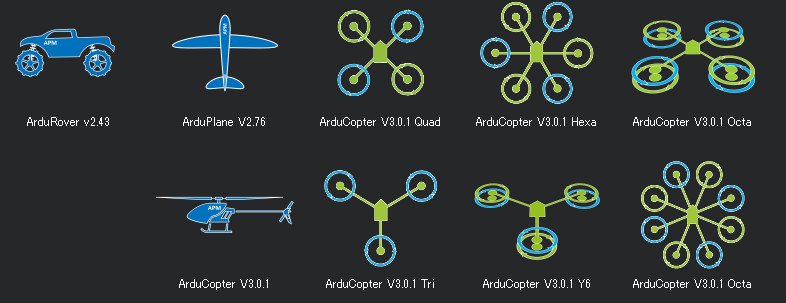
\includegraphics[width=0.8\textwidth] {images/arduScreenshot.jpg}
\caption{Screenshot der verschiedenen Firmwarevarianten.}
\label{fig:arduScreenshot}
\end{figure}

Auch andere Projekte könnten von unserem System profititeren. Uplift Aero beispielsweise, ist ein Startup, dass Hilfsgüter mit Hilfe von Drohnen von der Türkei aus nach Syrien fliegen wollte. Sie haben für ihre Flugzeuge (Grafik \ref{fig:uplift}) die selben Flugcontroller wie wir verwendet, mussten lediglich eine andere Firmware aufspielen. Dies beweist wie flexibel und vielseitig die von uns eingesetzte Hardware verwendet werden kann.

\begin{figure}[H]
\centering
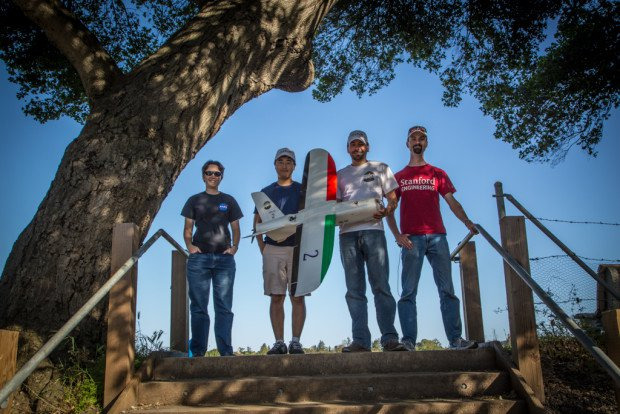
\includegraphics[width=0.8\textwidth] {images/SyriaUplift.jpg}
\caption{Uplift Team und die Syrien-Drohne Quelle: \protect\url{http://uplift.aero/}}
\label{fig:uplift}
\end{figure}





\chapter{Zusammenfassung und Ausblick}

\section{Impressionen der Ergebnisse}

Um den Einstieg für die Zielgruppe zu erleichtern, wurde eine Webseite erstellt, die die wichtigsten Funktionen erklärt und eine Übersicht über die Funktionsweise der Plattform bietet.

\begin{figure}[H]
	\centering
	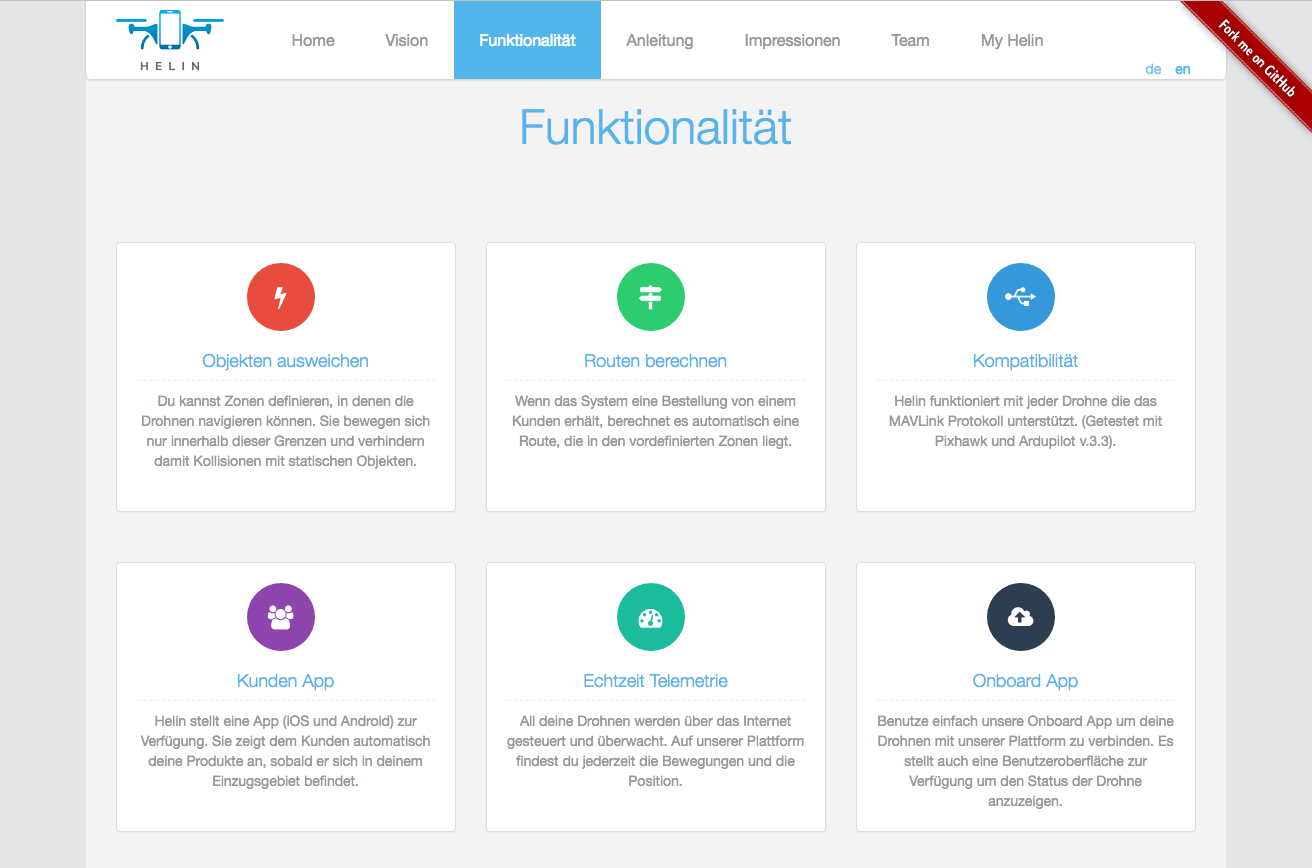
\includegraphics[width=1\textwidth] {images/website.png}
	\caption{Ausschnitt der Webseite \url{https://my.helin.ch/}}
\end{figure}
\newpage

Ausserdem wurde die Plattform auf \url{https://my.helin.ch/} freigeschaltet und kann frei genutzt werden.

\begin{figure}[H]
	\centering
	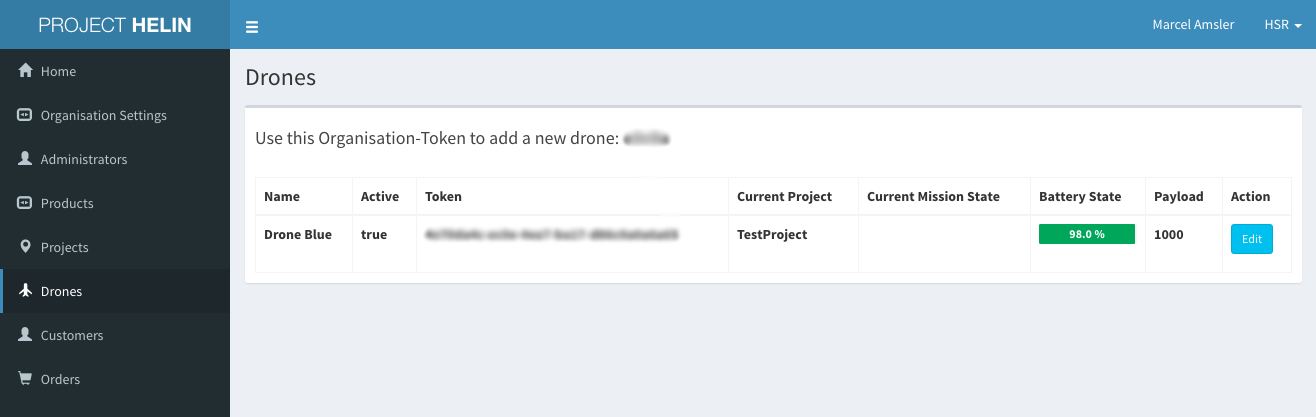
\includegraphics[width=1.0\textwidth] {images/myhelin.png}
	\caption{Drohnenliste von MyHelin}
\end{figure}

Die \Gls{Single-Page-Applications} für das Zeichnen von Zonen, das Testen eines Zonensetups und die Überwachung der Lieferungen stehen dann sofort zur Verfügung.

\begin{figure}[H]
	\centering
	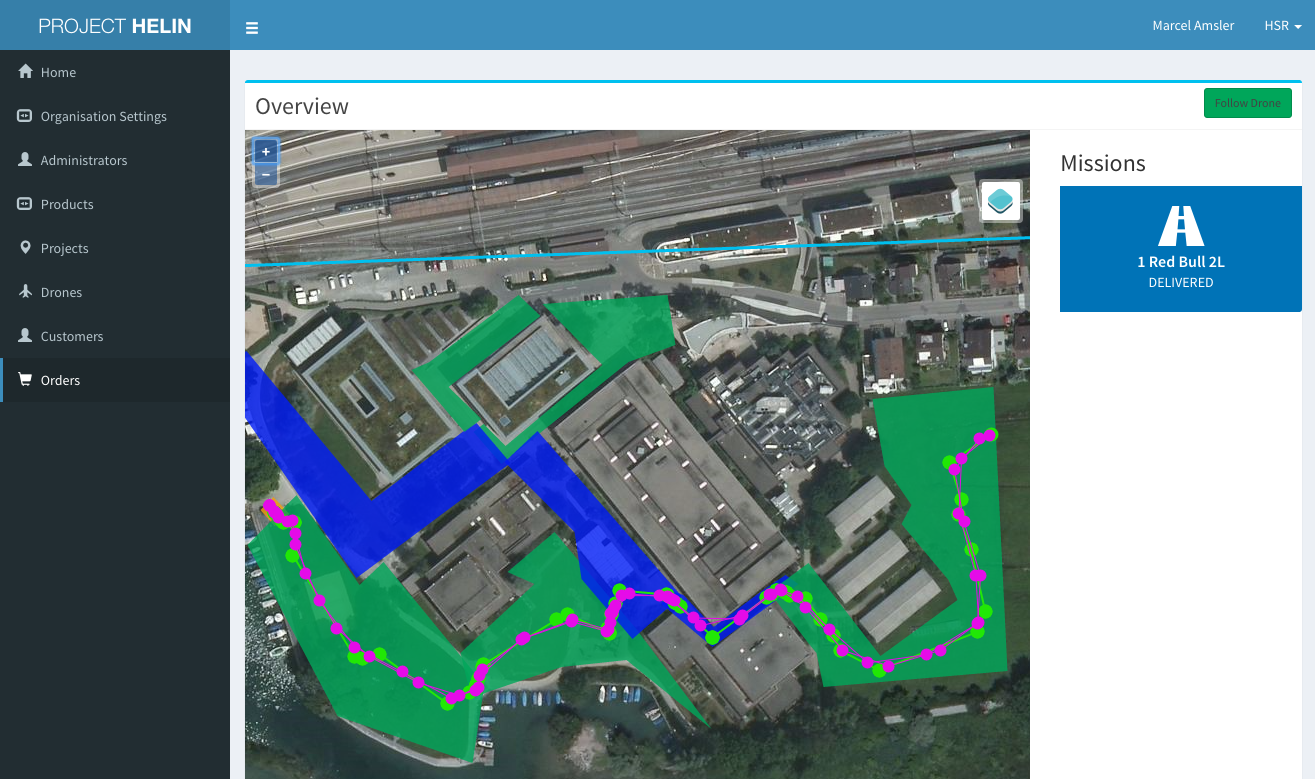
\includegraphics[width=1.0\textwidth] {images/map-ui.png}
	\caption{Kartenansicht bei der Verfolgung einer Drohne während der Mission}
\end{figure}

\newpage
Das Customer-App für Android (links), das Customer-App für iOS (mitte) und das Onboard-App (rechts) können verwendet werden.

\begin{figure}[H]
	\centering
	\begin{minipage}[b]{0.2\textwidth}
			\centering
		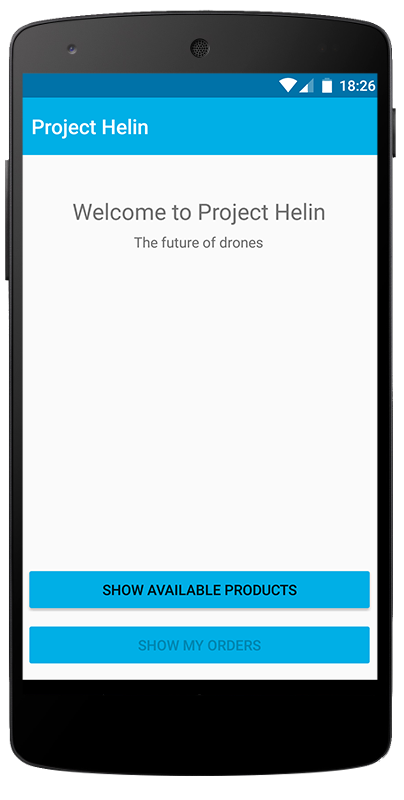
\includegraphics[width=\textwidth]{images/customer-app-android.png}
		\label{fig:customer-app-android}
	\end{minipage}
	\hfill
	\begin{minipage}[b]{0.2\textwidth}
		\centering
		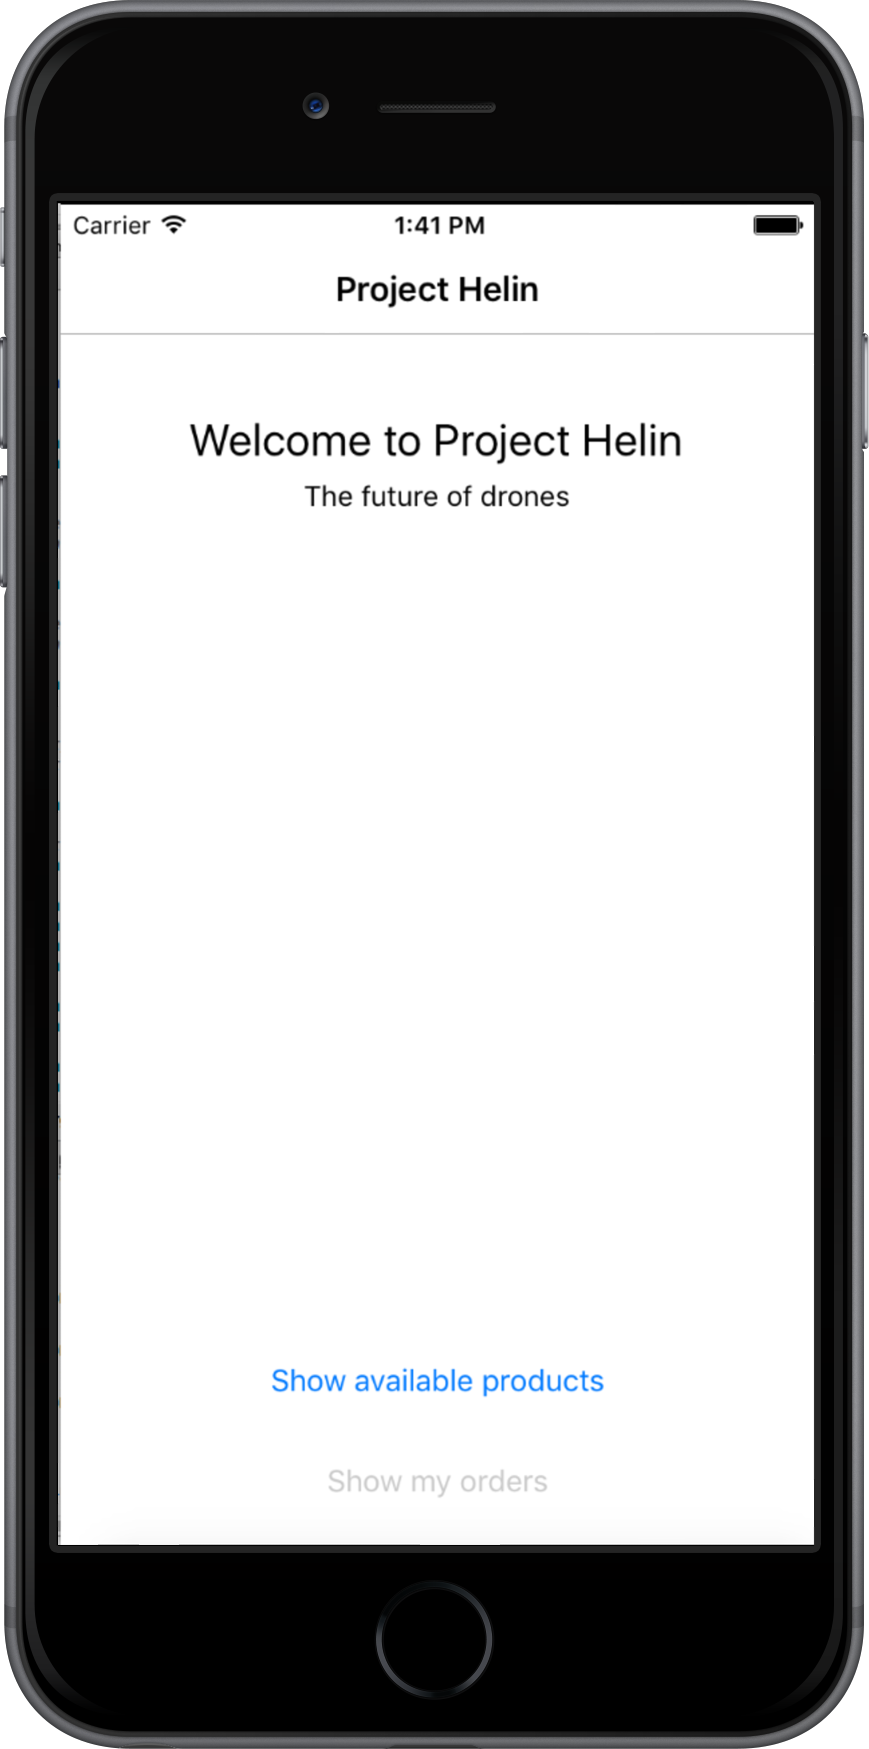
\includegraphics[width=\textwidth]{images/customer-app-ios.png}
		\label{fig:customer-app-ios}
	\end{minipage}
	\hfill
	\begin{minipage}[b]{0.2\textwidth}
			\centering
		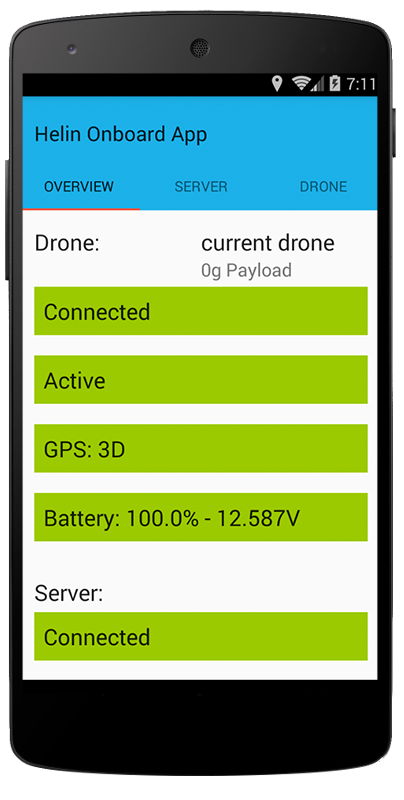
\includegraphics[width=\textwidth]{images/onboard-app.png}
		\label{fig:onboard-app-android}
	\end{minipage}
\end{figure}


Die Drohne zusammen mit dem Onboard-App konnte auf einen Stand gebracht werden, mit dem sie mehrere Lieferungen hintereinander ohne Schwierigkeiten ausführen kann.

\begin{figure}[H]
	\centering
	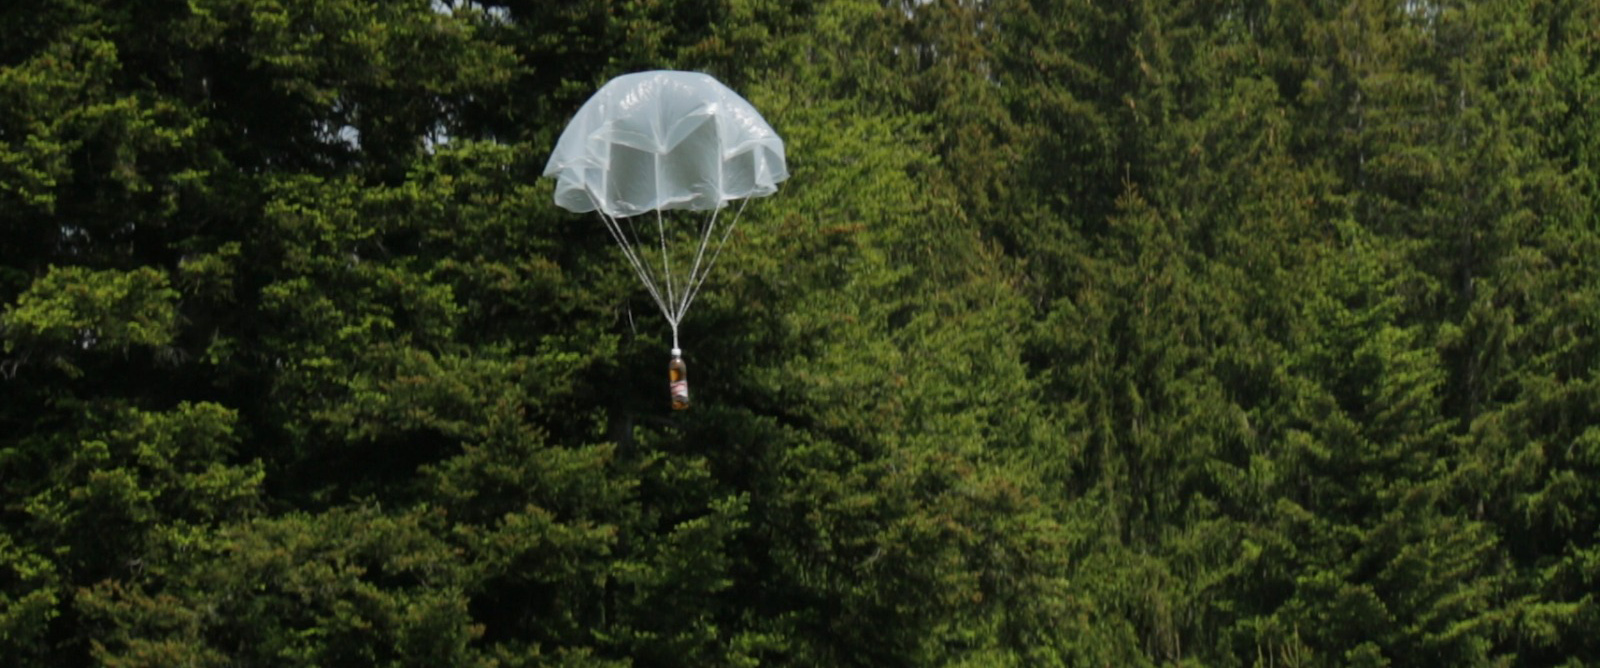
\includegraphics[width=1.0\textwidth] {images/parachute-test.jpeg}
	\caption{Diverse erfolgreiche Tests mit dem autonomen Abwurf der Ladung}
\end{figure}

\begin{figure}[H]
	\centering
	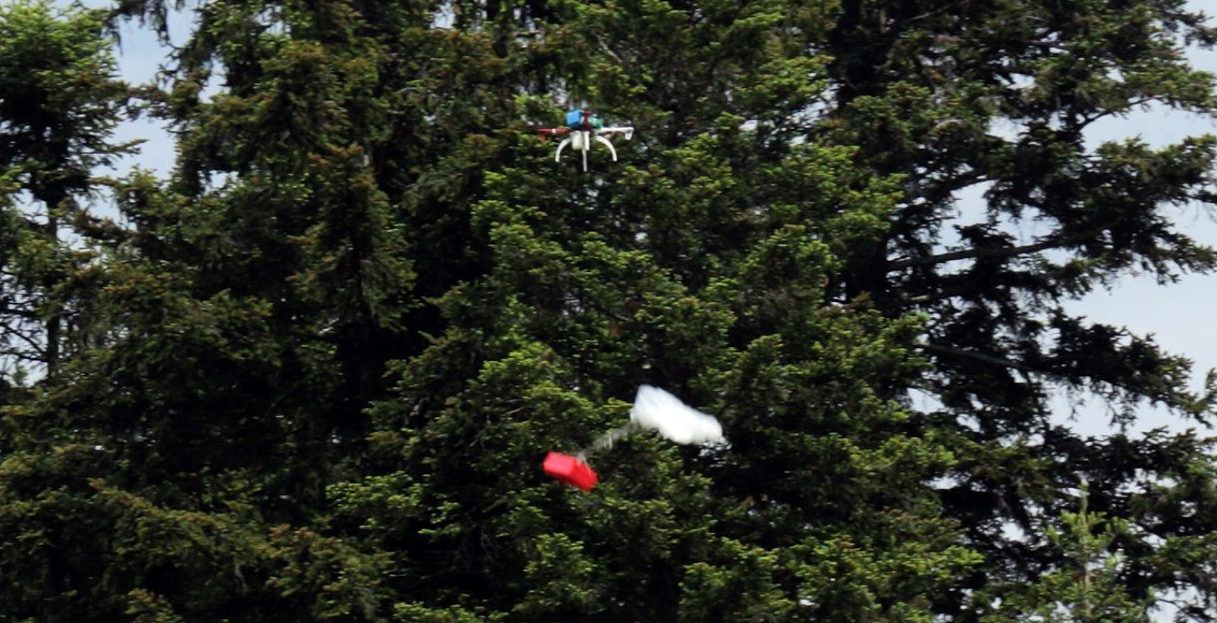
\includegraphics[width=0.95\textwidth] {images/drone-drop.jpg}
	\caption{Liefertest mit einem Verbandskasten}
\end{figure}
\begin{figure}[H]
	\centering
	\includegraphics[width=0.95\textwidth] {images/drone-drop2.jpg}
	\caption{Liefertest nach dem Öffnen des Fallschirms}
\end{figure}


\begin{figure}[H]
	\centering
	\includegraphics[width=1.0\textwidth] {images/drone.jpg}
	\caption{Drohne mit Onboard-App in der finalen Ausbaustufe}
\end{figure}


\newpage
\subsection{Zusammenfassung der Ergebnisse}

Während dieser Arbeit hat das Team eine Plattform konzipiert und entwickelt, die es jedem Anbieter ermöglicht, einen autonomen Drohnen-Lieferservice für ein von ihm definiertes Gebiet aufzubauen. Die Plattform wurde auf einem Server als Software as a Service zur Verfügung gestellt. Ausserdem wurde der gesamte Code des Projekts auf GitHub veröffentlicht und steht unter einer \Gls{MIT-Lizenz} als Open Source Software zur Verfügung. Die Tests mit den zwei eigens aufgebauten Drohnen zeigen, dass das System als Ganzes funktioniert. \\

Folgende Ergebnisse sind besonders hervorzuheben:

\begin{itemize}
	\item Webseite für Administratoren zur Verwaltung von Organisationen, Drohnen, Produkten und Bestellungen
	\item Cross-Plattform Bestell-App (iOS, Android) für Kunden
	\item Android App zur Steuerung der Drohne über das Internet
	\item Verfolgung der Drohnen-Telemetrie während, vor und nach der Lieferung einer Bestellung
	\item Automatisierte dynamische Routenberechnung über vordefinierte Flugzonen, abhängig von der Position des Kunden
	\item Automatisierte Verteilung von Lieferaufträgen an die Drohnen
	\item Getestete Vorlage für den Aufbau einer Lieferdrohne
	\item Vorgefertigte 3D-Modelle für den 3D-Druck der Smartphone-Halterung und der Abwurfvorrichtung
\end{itemize}

\newpage
\section{Ausblick}

Die entwickelte Plattform zeigt erst einen Bruchteil der Möglichkeiten, die in Zukunft von autonomen Drohnen übernommen werden können. Beispielsweise können Videoaufnahmen, Infrastruktur-Überwachung oder Katastrophenhilfe als Angebote integriert werden. 

\subsection{Empfohlene Weiterentwicklungen}

Während des Projekts sind weitere Ideen entstanden: 

\subsubsection{Plattform}

\begin{itemize}
	\item Services hinzufügen (Drone-Selfie, Follow-Me Video, geographische Vermessung)
	\item Aktion am Zielort wählbar oder vom Produkt abhängig machen
	\item Test, ob es auch mit Radio-Telemetry am Onboard-App funktioniert
	\item \Gls{Flight-Controller} ohne \Gls{MAVLink} auch unterstützen (z.B. DJI-Onboard-SDK \cite{dji-sdk})
	\item Globale Flugzonen die in allen Projekten sichtbar sind
	\item Kollisionsvermeidung von Drohnen auf denselben Routen
	\item Objekte mit Kollisionspotential (z.B. Gebäude, Bäume) automatisiert aus Flugzonen ausschliessen
\end{itemize}

\subsubsection{Drohnen Hardware} 
\begin{itemize}
	\item Testen in Kombination mit Obstacle Avoidance (z.B. Intel RealSense\cite{realsense}) Hardware
		\item Tests mit anderen Arten von Drohnen (siehe Abschnitt \ref{sec:drone-alternatives})
	\item Smartphone ersetzen durch Embedded-System (siehe Alternativen im Abschnitt \ref{sec:communication-architecture}) 

	\item Automatisches Beladungssystem für Drohnen
	\item Automatisches Batterieaustauschsystem für Drohnen
\end{itemize}  



\subsection{Known-Issues}

Alle bekannten kleineren Probleme und zusätzlichen Features, die vor einem produktiven Einsatz des Systems umgesetzt werden sollten, werden im Server-GitHub-Repository als Issues erfasst. Dies ermöglicht es auch anderen Entwicklern an dem Projekt weiterzuarbeiten und dessen Limitierungen zu kennen.

\newpage
\section{Schlussfolgerung}

Während dieser Arbeit haben wir aus unserer Vision ein Produkt entwickelt und fertiggestellt. Damit konnten wir beweisen, dass man mit verfügbaren Technologien Liefersysteme mit autonomen Drohnen schon heute realisieren kann. Die entstandene Plattform kann nun zu Testzwecken von allen Interessierten genutzt und weiterentwickelt werden.\\

Die erarbeiteten funktionalen- und nicht-funktionalen Anforderungen konnten alle erfüllt und teilweise übertroffen werden, trotz der vielfältigen und teilweise interdisziplinären Aufgaben, die dieser Arbeit innewohnten. \\

Unserer Meinung nach ist unsere Plattform ein Beispiel für die Drohnen-Projekte der Zukunft. Vor allem in Bezug auf die Verwendung einer zentralen Instanz, zur Steuerung und Überwachung einer Drohnenflotte. Dadurch gewinnen viele Projekte, wie das Überwachen von Haien \cite{shark}, die Lieferung von Defibrillatoren \cite{defibrillator-drone} oder das Finden von Überlebenden in einem Katastrophengebiet \cite{catastrophic-drone}, deutlich an praktischer Relevanz und können flächendeckend eingesetzt werden. Wir hoffen, dass die entwickelte Plattform als Anstoss für die Stakeholder in dieser Branche dienen kann und sich die Technologien und Gesetzeslagen insoweit verbessern, dass Dienstleistungen von autonomen Drohnen bald für eine grössere Anzahl von Kunden zur Verfügung stehen werden.







\part{Anhang}
\newpage
\renewcommand \thechapter{\Alph{chapter}}

\newpage

\chapter{Infrastruktur}

\section{Server}

Für die Helin Applikation wird ein physischer Server verwendet. Wie in der Abbildung \ref{fig:communication-architecture-overview} dargestellt, wird dieser als Build-, Test- und Applikations-Server verwendet. 
Auf dem Server läuft eine PostgreSQL Datenbank mit einer PostGIS Extension, welche für die Routenberechnung benötigt wird. Gleichzeitig ist ein RabbitMQ-Message-Broker und eine Instanz der Helin Server Applikation installiert. Aus Resourcengründen wird alles auf einem Server ausgeführt, könnte aber bei Leistungsproblemen ohne weiteres auf mehrere Server verteilt werden. Als Build- und Test-Server für alle Applikationen wird TeamCity verwendet. 

Neben dem Server werden auch Apps für Android Geräte veröffentlicht. Beide kommunizieren primär mit der RabbitMQ Instanz auf dem Server.

\begin{figure}[h]
	\includegraphics[width=1.0\textwidth]{images/DeploymentDiagram.png}
	\caption{Deployment Diagram}
	\label{fig:deployment-diagram}
\end{figure}




\definecolor{boxred}{RGB}{234,99,99}
\definecolor{boxorange}{RGB}{255,242,204}
\definecolor{boxgreen}{RGB}{217,234,211}


\newcommand{\greenbox}{
\begin{tikzpicture}
\draw[line width=0pt, fill=boxgreen]
(0, 0) rectangle (0.3, 0.3);
\end{tikzpicture}}

\newcommand{\orangebox}{
\begin{tikzpicture}
\draw[line width=0pt, fill=boxorange]
(0, 0) rectangle (0.3, 0.3);
\end{tikzpicture}}

\newcommand{\redbox}{
\begin{tikzpicture}
\draw[line width=0pt, fill=boxred]
(0, 0) rectangle (0.3, 0.3);
\end{tikzpicture}}


\chapter{Projektplan}
\section{Änderungsgeschichte}
\begin{tabularx}{\textwidth}{|c|c|X|c|}
  \hline
  \textbf{Datum} & \textbf{Version} & \textbf{Änderung} & \textbf{Autor} \\
  \hline \hline
  26.02.2016 & 1.0 & Erstellen des Projektplans & Martin Stypinski \\
  \hline
\end{tabularx}

\section{Einleitung}
\subsection{Ziel und Zweck}
Ziel dieser Arbeit ist es, eine Web-Applikation zu entwickeln, die es ermöglicht Drohnenflotten zu verwalten und damit vollautomatisierte Lieferungen auszuführen. Nutzer dieser Applikation können dazu Flugzonen definieren, in denen ein sicherer Flug von Drohnen möglich ist. Kunden hingegen sollen durch eine App die Möglichkeit erhalten, Güter zu bestellen, welche an ihre aktuelle Position ausgeliefert werden.

\subsection{Lieferumfang}
Der Lieferumfang dieser Arbeit entspricht den Vorgaben der HSR:
\begin{itemize}
	\item{Zu Handen des Betreuers:
	\begin{itemize}
		\item{Ein gedrucktes Exemplar der Dokumentation}
		\item{Dokumentation, sämtliche Dokumente und Sourcen auf CD}
	\end{itemize}}
	\item{Poster - Enthält Zusammenfassung der Arbeit}
	\item{Abstract für die Bachelorarbeitsbrochure}
\end{itemize}
Zusätzlich ist es uns ein Anliegen, dass der Sourcecode und die Erfahrungen über den Zeitraum der Bachelorarbeit hinaus bestehen bleiben. Daher wurde ein GitHub-Repository eingerichtet, dass nach Beendigung der Arbeit sämtliche Teile enthält: \textbf{\url{https://github.com/Project-Helin}}

\subsection{Annahmen und Einschränkungen}
Es kann angenommen werden, dass der Zeitplan im Rahmen der regulären Bachelorarbeit Zeit gültig ist. Es wird dabei berücksichtigt das ein Zeithorizont von 17 Wochen zur Verfügung steht und die maximale Arbeitszeit von 360 Stunden pro Person nicht überschritten werden soll.

\newpage

\section{Projektorganisation}
\subsection{Organisationsstruktur}
\begin{figure}[ht]
%\begin{figure}[H]
	\centering
	\includegraphics[width=\textwidth]{images/organigram.png}
	\caption{Grobübersicht über den Projektplan}
	\label{Risk result}
\end{figure}
\noindent
\begin{tabularx}{\textwidth}{|c|c|X|}
  \hline
  \textbf{Name} & \textbf{E-Mail} & \textbf{Verantwortung} \\
  \hline \hline
  Prof. Dr. Markus Stolze & \url{markus.stolze@hsr.ch} & Betreuer der Arbeit\\
  \hline \hline
  Marcel Amsler & \url{marcel.amsler@hsr.ch} & \\
  \hline
  Kirusanth Poopolasingam & \url{kirusanth.poopalasingam@hsr.ch} & \\
  \hline
  Martin Stypinski & \url{martin.stypinski@hsr.ch} & \\
  \hline
\end{tabularx}
\subsection{Meetings}
In der Regel wird ein Meeting jeweils am Donnerstag um 10.30 in der Mensa abgehalten. In Ausnahmefällen können die Termine von der Planung abweichen.
  \\[1\normalbaselineskip]
\begin{tabularx}{\textwidth}{|c|c|c|X|}
  \hline
  \textbf{SW} & \textbf{Datum} & \textbf{Zeit} & \textbf{Art der Sitzung} \\
  \hline \hline
  1 & 25.02.2016 & 10:00 - 11:00 &  Kick-off meeting \\
  2 & 03.03.2016 & 15:00 - 16:00 &  Meeting mit Betreuer \\
  \hline
\end{tabularx}
\newpage
\section{Meilensteinplanung}
Grundsätzlich wird während der gesamten Arbeit Agiles-Projektmanagement mit Scrum als Methode eingesetzt. Ein Scrum-Sprint dauert in der Regel 2 Wochen. Die Meilensteine dienen nur zu Priorisierungszwecken.

\begin{figure}[ht]
%\begin{figure}[H]
	\centering
	\includegraphics[width=\textwidth]{images/projplan.png}
	\caption{Grobübersicht über den Projektplan}
	\label{Risk result}
\end{figure}

\begin{itemize}
	\item{\textbf{Ende Einarbeitung: (MS-1)} 
		\begin{itemize}
			\item{\textbf{Datum:} 11.03.2016}
			\item{\textbf{Ziel:} Entwicklungsumgebung und Prozesse stehen.}
			\item{\textbf{Erfüllungskriterium:} Sämtliche prozessbegleitenden Massnahmen sind lauffähig. Projektmanagement-Tool, IDEs, CI}
		\end{itemize}
	}
	
	\item{\textbf{Ende Proof of Concept: (MS-2)} 
		\begin{itemize}
			\item{\textbf{Datum:} 25.03.2016}
			\item{\textbf{Ziel:} Die Machbarkeit ist bewiesen.}
			\item{\textbf{Erfüllungskriterium:} Prototyp ist lauffähig, zeigt Machbarkeit und allfällige Einschränkungen.}
		\end{itemize}
	}
	
	\item{\textbf{Ende Implementierung: (MS-3)} 
		\begin{itemize}
			\item{\textbf{Datum:} 03.06.2016}
			\item{\textbf{Ziel:} Code Freeze}
			\item{\textbf{Erfüllungskriterium:} Alle zwingenden funktionalen- und nicht-funktionalen Anforderungen sind erfüllt.}
		\end{itemize}
	}	
	\item{\textbf{Abgabe: (MS-4)} 
			\begin{itemize}
				\item{\textbf{Datum:} 17.06.2016}
				\item{\textbf{Ziel:} Abgabe der Arbeit}
				\item{\textbf{Erfüllungskriterium:} Alle im Lieferumfang geforderten Dokumente sind fertiggestellt.}
			\end{itemize}
	}
	
\end{itemize}

\newpage


\begin{landscape}
\section{Risikomanagement}
\subsection{Risiken}
\LTXtable{0.75\paperheight}{risk.tex}
\end{landscape}
\subsection{Umgang mit Risiken}
Die Risken wurden in einer Risiko Matrix aufgegliedert um besser zu verstehen, welche Risiken eine grosse Bedrohung darstellen.

\begin{figure}[ht]
%\begin{figure}[H]
	\centering
	\includegraphics[scale=0.7]{images/risk_result.png}
	\caption{Risiko Matrix}
	\label{Risk result}
\end{figure}

Als Konsequenz der Matrix kann folgende Aufteilung getroffen werden:
\begin{itemize}
	\item{\textbf{Risiko hoch:} R03, R06}
	\item{\textbf{Risiko mittel:} R01, R04, R05, R07, R08, R09, R10, R12 }
	\item{\textbf{Risiko klein:} R02, R11, R13, R14}
\end{itemize}
\subsection{Massnahmen}
Für die Risiken der Kategorie mittel und hoch wurden folgende Massnahmen festgelegt:
\begin{itemize}
	\item{\textbf{R03 - Internet auf Mobilgerät:} \\
	\textbf{Massnahmen:} Es muss sichergestellt werden, dass die Drohne nicht auf eine permanente Serververbindung angewiesen ist. Monitor und Datenlogging dürfen Unterbrechungen aufweisen. Die Mission darf aber zu keinem Zeitpunkt gefährdet werden, die Drohne muss selbstständig ihre Aufgabe erfüllen können und danach wieder zurückkehren.}
	
	\item{\textbf{R06 - Absturz und Schäden:} \\
	\textbf{Massnahmen:} Bei der Wahl der Drohne wurde auf die Verfügbarkeit der Ersatzteile geachtet, sofern dies möglich war. }

	\item{\textbf{R01 - JMS auf Mobilgerät:} \\
	\textbf{Massnahmen:} Bei der Evaluierung der Komponenten wird eine JMS Implementierung gewählt, die auf einem Android Betriebssystem lauffähig ist. Dies wird in einem Proof of Concept überprüft.}
	
	\item{\textbf{R04 - Infrastruktur Probleme:} \\
	\textbf{Massnahmen:} Auf Grund von Erfahrungen aus früheren Projekten, wird auf die Serverinfrastruktur der HSR verzichtet, dies garantiert eine volle Kontrolle über den Server. Es muss jedoch berücksichtig werden, dass der administrative Aufwand höher ist und somit mehr Zeit in Anspruch nehmen wird.}
	
	\item{\textbf{R05 - Kapazität der Drohne:} \\
	\textbf{Massnahmen:} Es werden Güter verwendet, deren Gewicht von der Drohne transportiert werden kann.}	
	
	\item{\textbf{R07 - Positionsungenauigkeit:} \\
	\textbf{Massnahmen:} Bei Flugkorridoren und Landepunkten wird genügend Sicherheitsmarge eingerechnet um die Ungenauigkeit zu relativieren.}
	
	\item{\textbf{R08 - Ardupilot Handhabung:} \\
	\textbf{Massnahmen:}  Im Proof of Concept wird überprüft, wann und wie Updates gemacht werden können. Falls Updates während des Flugs nicht möglich sind, wird von Anfang an die gesamte Route an Ardupilot übertragen.}
	
	\item{\textbf{R09 - Ardupilot API:} \\
	\textbf{Massnahmen:} Früh in einem Proof of Concept die Möglichkeiten und Grenzen des APIs nachvollziehen.}
	
	\item{\textbf{R10 - Entwicklungsprozesse:} \\
	\textbf{Massnahmen:} Es wird während des Proof of Concepts versucht einen Simulator zu verwenden um Zeit zu sparen. Gegebenenfalls Arbeitsplatz im Freien, um Zeit während des Deployments auf die Drohne zu sparen.}
	
	\item{\textbf{R12 - Ablademanagement:} \\
	\textbf{Massnahmen:} Prüfung einer Abwurfmöglichkeit. Gegebenenfalls Benutzer mit GUI auf Mobile begleiten um einen sicheren und unfallfreien Ablad zu garantieren.}
\end{itemize}

\section{Qualitätsmassnahmen}	
\subsection{Dokumentation}
Die Dokumentation wird vollständig in Latex geschrieben und befindet sich zu jedem Zeitpunkt auf dem Project-Helin GitHub-Repository: \url{http:www.github.com/project-helin}. Alle grösseren Änderungen werden immer von einem anderen Teammitglied gelesen und überprüft.

\subsection{Projektmanagement}
Für das Projektmanagement wird Jira von Atlassian verwendet. \\
Als Projektmanagmenet Methodik wird Scrum verwendet, jedoch werden einige Meilensteine gesetzt um den Fokus nicht aus den Augen zu verlieren und sich über Teilziele bewusst zu sein.

\subsection{Entwicklung}
Die Qualität der Entwicklung wird durch folgende Massnahmen sichergestellt:
\begin{itemize}
	\item{\textbf{Code Review:} Bei kritischen Komponenten werden Code Reviews durchgeführt.}
	
	\item{\textbf{Feature Review:} Bei allen Features bzw. umgesetzten User-Stories führt ein anderes Teammitglied eine Qualitätskontrolle durch. Diese kontrolliert hauptsächlich die Erfüllung der Acceptance-Criterias.}
	
	\item{\textbf{Testing:} Das gesammte Projekt wird in Java entwickelt. Als Unit-Test Framework JUnit4 verwendet.}
	
	\item{\textbf{Versionierung:} Der gesammte Quellcode wird mit Hilfe von GitHub versioniert.}
	
	\item{\textbf{Deployment:} Die Serverkomponenten werden mithilfe eines Build Systems deployt. Die Komponenten auf den Mobiltelefonen werden manuell deployt. Jedoch wird auf dem Build-System für alle Komponenten die Ausführung von Unit-Tests garantiert.}
	
\end{itemize}

\newpage
\section{Systemtests}	

Die nachfolgenden Tests wurden mit den folgenden Komponenten durchgeführt: 

\begin{itemize}
	\item Server befindet sich auf www.helin.ch
	\item On-Board-App: läuft auf einem Nexus 4 mit Android 4.4
	\item Customer-App: läuft auf einem Neuxs 5 mit Android 6.1
	\item Customer-App wurde mit einem OTG Kabel an der Drohne verbunden
\end{itemize}

\subsection{Administrations Seite}	
\subsubsection{Funktionale Anforderungen}	
\begin{todolist}
	\item[\done] Es kann ein Administrator Account erstellt werden
	\item[\done] Es kann kein Account mit demselben Namen erstellt werden
	\item[\done] Administrator kann sich mit seinem Email und Passwort einloggen
	\item[\done] Administrator kann eine neue Organisation erstellen
	\item[\done] Administrator kann den Namen der Organisation ändern
	\item[\done] Administrator kann einen zusätzlichen Administrator zur Organisation hinzufügen
	\item[\done] Es kann ein Administrator aus der Organisation gelöscht werden
	\item[\done] Administrator kann ein neues Produkt erfassen
	\item[\done] Administrator kann ein vorhandenes Produkt editieren
	\item[\done] Administrator kann ein Produkt löschen
	\item[\done] Administrator kann ein neues Projekt erfassen
	\item[\done] Administrator kann ein Produkt erfassen
	\item[\done] Administrator kann eine Bestell-, Abwurfs-, Flug- und Ladezone definieren
	\item[\done] Administrator kann eine Zone anpassen und löschen
	\item[\done] Administrator kann ein Produkt zu einem Projekt zuweisen
	\item[\done] Administrator kann ein Produkt aus einem Projekt herauslöschen
	\item[\done] Administrator kann eine Test Flugroute generieren.

	\item[\done] Administrator kann die Bestellung ansehen.
	\item[\done] Administraotr kann die vorgeschlagene und geflogene Flugroute anschauen.

	\item[\done] Eine registrierte Drohne kann einem Projekt zugewiesen werden
	\item[\done] Eine registrierte Drohne kann angepasst werden
	\item[\done] Eine registrierte Drohne kann als inaktiv markiert werden
	\item[\done] Eine aktuell verbundene Drohne zeigt den letzten Akku stand an.

	\item[\done] Administrator kann alle Bestellungen ansehen
	\item[\done] Administrator kann die Missionen pro Bestllung ansehen
	\item[\xmark] Administrator kann eine Bestellunge ändern ( Funtkionale Anforderung )
	\item[\xmark] Administrator kann eine Bestellunge löschen ( Funtkionale Anforderung )

	\item[\xmark] Drohne kann herausgelöscht werden (Funktionale Anforderung)
	\item[\xmark] Administrator kann eine laufende Mission abbrechen
	\item[\xmark] Administrator kann Services definieren ( Funktioanle Anforderung )

\end{todolist}

\subsubsection{Nicht-Funktionale Anforderungen}	
\begin{todolist}
	\item[\done] Auf die Seite kann nur über HTTPS zugegriffen werden
\end{todolist}

\subsection{Drone-Operator}	
\subsubsection{Funktionale Anforderungen}	
\begin{todolist}
	\item[\done] Das OnBoard-App kann über ein APK heruntergeladen und installiert werden.
	\item[\done] Mit dem OnBoard-App kann ich die Drohne beim Server registrieren und einer Organisation hinzufügen
	\item[\done] Das OnBoard-App kann sich mit dem Server verbinden
	\item[\done] Das OnBoard-App kann auf Wunsch die Verbindung zum Server trennen
	\item[\done] Die Drohne kann auf dem OnBoardApp als inaktiv markiert werden
	\item[\done] Das OnBoard-App kann sich mit der Drohne über USB Kabel verbinden
	\item[\done] Das OnBoard-App kann die Verbindung mit der Drohne trennen
	\item[\done] Es kann der aktuelle Status des GPS, Batterie Status und der Verbindung zum Server angezeigt werden
	\item[\done] Eine vorgeschlagene Mission kann abgelehnt werden
	\item[\done] Drone-Operator kann eine Mission annehmen und sieht die zu belandende Produkte
	\item[\done] Bevor die Drohne startet erhalten ich eine Countdown
	\item[\done] Bevor die Drohne startet erhalte ich einen akustischen Signal 
	\item[\done] Während des Countdown kann der Start abgerochen werden
	\item[\done] Die Drohne kann mit den Produkten beladen und bestätigt werden
\end{todolist}

\subsubsection{Nicht-Funktionale Anforderungen}	
\begin{todolist}
	\item[\done] Die Verbindung zum Server beim Registrieren ist verschlüsselt ( Server kann nur https)
	\item[\done] Die Verbindung zum Server bei der Übertragung der Drohneninformation ist verschlüsselt (überprüft mittels RabbitMQ Management Konsole)
	\item[\done] Beim Verbindungsabbruch zum Server wird die Mission weitergeführt
	\item[\done] Nach einem Verbindungsabbruch wird die Verbindung automatisch wiederhergestellt
\end{todolist}

\subsection{Customer}	
\subsubsection{Funktionale Anforderungen}	
\begin{todolist}
	\item[\xmark] Der Kunde kann sich die App aus dem Google Play Store herunterladen
	\item[\done] Kunde kann sich die bestellbaren Produkte anschauen, ohne sich einzuloggen
	\item[\done] Kunde sieht nur nur Produkte innerhalb der Bestellzone
	\item[\done] Kunde kann eine Bestellung abschicken und sieht die voraussichtliche Lieferposition
	\item[\done] Kunde kann die Bestellung abbrechen
	\item[\done] Kunde kann sich über Google Anmelden und sieht welche Berechtigung von Google erforderlich sind
	\item[\done] Kunde kann die bestellte Ware mit PayPal bezahlen ( nur im Testmodus )
	\item[\done] Kunde kann die Bestellung bestätigen
	\item[\done] Kunde kann die seine Bestellungen anschauen und dessen Status ansehen
	\item[\done] Kunde kann die einzelnen Lieferung anschauen und dessen Status ansehen
	\item[\done] Kunde kann bei einer aktuellen Lieferung die Position der Drohne mitverfolgen
	\item[\xmark] Als Kunde kann ich  eine Bestellung stornieren
\end{todolist}

\subsubsection{Nicht-Funktionale Anforderungen}	
\begin{todolist}
	\item[\done] Die Verbindung zum Server ist verschlüsselt
	\item[\done] Ohne Internetverbindung wird beim Abruf der Produkte eine Fehlermeldung angzeigt.
	\item[\done] Ohne GPS Verbindung wird beim Abruf der Produkte eine Fehlermeldung angzeigt.
\end{todolist}



\chapter{Code Standards}
Im Team wurden folgende Code-Conventions eingeführt.

\subsubsection{Autorfreie Klassen}
In Java wird klassicherweise der Autor im Javadoc Kommentar in der Klasse angegeben.

\begin{lstlisting}
/**
 * @author Kirusanth Poopalasingam (pkirusanth@gmail.com)
 */
public class MyTestClass{
}
\end{lstlisting}
Der Autor in der Klasse suggeriert, dass nur ein Autor für diese Klasse existiert und für diese Klasse verantwortlich ist. Dies sollte aber nicht der fall sein, da jedes Teammitglied verantwortlich für die gesamte Code-Qualität ist und zudem ist die Angabe auf der Klasse heutzutage mit einem Version Control System redundant.

\subsubsection{Javadoc}
Generell sollte Javadoc nur dort verwendet werden, wo es nötig ist. Da es sich bei Projekt Helin nicht um eine API handelt, sollten auch die Methoden und Parameter nicht redundant dokumentiert werden. Ein Beispiel für eine schlechte Javadoc Dokumentation sieht folgendermassen aus:
\begin{lstlisting}
// Beispiel einer Play Klasse
public final class ConfigUtil {
    private ConfigUtil() { }

    /**
     * Quotes and escapes a string, as in the JSON specification.
     *
     * @param s
     *            a string
     * @return the string quoted and escaped
     */
    public static String quoteString(String s) {
        return ConfigImplUtil.renderJsonString(s);
    }
    // ...
}
\end{lstlisting}
Bei der Methode quoteString() kann der ganze Javadoc Kommentar weggelassen werden, da er nicht mehr Aussagekraft hat, als die Methode selbst. Stattdessen sollte die Methode so geschreiben werden, dass die Namen aussagekräftiger sind.
\\
Eine bessere Implementierung würde folgendermassen aussehen:
\begin{lstlisting}
public final class ConfigUtil {
    private ConfigUtil() { }

    public static String quoteStringAccordingToJsonSpecification(String unquotedJson) {
        return ConfigImplUtil.renderJsonString(unquotedJson);
    }
    // ...
}
\end{lstlisting}
\subsubsection{Code}
Für die Formatierung und den Static Check werden die 'Code Inspection' von IntelliJ IDEA verwendet.
\\
Es handelt sich bei den 'Code Inspections' um konfigurierbare Regeln, welche mit dem Projekt in das Repository eingecheckt werden (code-style.xml). Die Entwicklungsumgebung führt die 'Code Inspections' vor dem Einchecken aus und weist gegebenenfals auf Unstimmigkeiten hin.
Da sich die standard Regeln von IntelliJ bereits in anderen Projekten bewährt haben, wurde von einem eigenen Standard abgesehen.
\newpage

\newpage
\chapter{Systemtest}

Die nachfolgenden Tests wurden mit den folgenden Komponenten durchgeführt:

\begin{itemize}
	\item Server befindet sich auf www.helin.ch
	\item On-Board-App: läuft auf einem Nexus 4 mit Android 4.4
	\item Customer-App: läuft auf einem Nexus 5 mit Android 6.1
	\item Customer-App wurde mit einem OTG Kabel mit der Drohne verbunden
\end{itemize}

Es wurde jeweils nach dem Implementierungs-Meilensteinen ein kompletter Test ausgeführt.

\section{Ende Proof Of Concept}

Die Tests wurden am 25.03.2016 durchgeführt.

\begin{todolist}
	\item[\done] Der Administrator kann sich erfolgreich registrieren.
	\item Es kann kein Account mit demselben Namen erstellt werden
	\item[\done] Administrator kann sich mit seinem Email und Passwort einloggen
	\item[\done] Administrator kann eine neue Organisation erstellen
	\item[\done] Administrator kann den Namen der Organisation ändern
	\item Administrator kann einen zusätzlichen Administrator zur Organisation hinzufügen
	\item Es kann ein Administrator aus der Organisation gelöscht werden
	\item[\done] Administrator kann ein neues Produkt erfassen
	\item[\done] Administrator kann ein vorhandenes Produkt editieren
	\item[\done] Administrator kann ein Produkt löschen
	\item[\done] Administrator kann ein neues Projekt erfassen
	\item Administrator kann eine Bestell-, Abwurfs-, Flug- und Ladezone definieren
	\item Administrator kann eine Zone anpassen und löschen
	\item Administrator kann ein Produkt zu einem Projekt zuweisen
	\item Administrator kann ein Produkt aus einem Projekt herauslöschen
	\item Administrator kann eine Flugroute mit einem Kunden simulieren.
	
	\item Administrator kann die Bestellung ansehen.
	\item Administrator kann die vorgeschlagene und geflogene Flugroute anschauen.
	
	\item[\done] Eine registrierte Drohne kann einem Projekt zugewiesen werden
	\item Eine registrierte Drohne kann angepasst werden
	\item Eine registrierte Drohne kann als inaktiv markiert werden
	\item Eine aktuell verbundene Drohne zeigt den letzten Akku stand an.
	\item Administrator kann alle Bestellungen ansehen
	\item Administrator kann die Missionenen einer Bestellung ansehen
	
	\item Administrator kann eine Bestellung ändern ( Funtkionale Anforderung )
	\item Administrator kann eine Bestellung löschen ( Funtkionale Anforderung )
	\item Drohne kann herausgelöscht werden (Funktionale Anforderung) 
	
	\item Administrator kann eine laufende Mission abbrechen 
\end{todolist}

\subsubsection{Nicht-Funktionale Anforderungen}
\begin{todolist}
	\item Auf die Seite kann nur über HTTPS zugegriffen werden
\end{todolist}

\subsection{Drone-Operator}
\subsubsection{Funktionale Anforderungen}
\begin{todolist}
	\item Das Onboard-App kann über ein APK heruntergeladen und installiert werden.
	\item[\done] Mit dem Onboard-App kann ich die Drohne beim Server registrieren und einer Organisation hinzufügen
	\item[\done] Das Onboard-App kann sich mit dem Server verbinden
	\item Das Onboard-App kann auf Wunsch die Verbindung zum Server trennen
	\item Die Drohne kann auf dem Onboard-App als inaktiv markiert werden
	\item[\done] Das Onboard-App kann sich mit der Drohne über USB Kabel verbinden
	\item[\done] Das Onboard-App kann die Verbindung mit der Drohne trennen
	\item Es kann der aktuelle Status des GPS, der Batterie und der Verbindung zum Server angezeigt werden
	\item Eine vorgeschlagene Mission kann abgelehnt werden
	\item Drone-Operator kann eine Mission annehmen und sieht die zu belandende Produkte
	\item Bevor die Drohne startet erhalte ich einen Countdown
	\item Bevor die Drohne startet erhalte ich einen akustisches Signal
	\item Während des Countdowns kann der Start abgebrochen werden
	\item Die Drohne kann mit den Produkten beladen und bestätigt werden
\end{todolist}

\subsubsection{Nicht-Funktionale Anforderungen}
\begin{todolist}
	\item Die Verbindung zum Server beim Registrieren ist verschlüsselt ( Server kann nur HTTPS angesprochen werden )
	\item Die Verbindung zum Server bei der Übertragung der Drohneninformation ist verschlüsselt (überprüft mittels RabbitMQ Management Konsole)
	\item[\done] Beim Verbindungsabbruch zum Server wird die Mission weitergeführt
	\item[\done] Nach einem Verbindungsabbruch wird die Verbindung automatisch wiederhergestellt
\end{todolist}

\subsection{Customer}
\subsubsection{Funktionale Anforderungen}
\begin{todolist}
	\item Der Kunde kann sich die App aus dem Google Play Store herunterladen 
	\item Kunde kann sich die bestellbaren Produkte anschauen, ohne sich einzuloggen
	\item Kunde sieht nur nur Produkte innerhalb der Bestellzone
	\item Kunde kann eine Bestellung abschicken und sieht die voraussichtliche Lieferposition
	\item Kunde kann die Bestellung abbrechen
	\item Kunde kann sich über Google Anmelden und sieht welche Berechtigung von Google erforderlich sind
	\item Kunde kann die bestellte Ware mit PayPal bezahlen ( nur im Testmodus )
	\item Kunde kann die Bestellung bestätigen
	\item Kunde kann seine Bestellungen anschauen und dessen Status ansehen
	\item Kunde kann die einzelnen Lieferung anschauen und dessen Status ansehen
	\item Kunde kann bei einer aktuellen Lieferung die Position der Drohne mitverfolgen
	\item Als Kunde kann ich  eine Bestellung stornieren
\end{todolist}

\subsubsection{Nicht-Funktionale Anforderungen}
\begin{todolist}
	\item Die Verbindung zum Server ist verschlüsselt
	\item Ohne Internetverbindung wird beim Abruf der Produkte eine Fehlermeldung angzeigt
	\item Ohne GPS Verbindung wird beim Abruf der Produkte eine Fehlermeldung angzeigt
\end{todolist}



\section{Ende Implementierung}

Dies folgenden Tests wurden, nach dem Abschluss der Implementierung durchgeführt, am 06.06.2016 durchgeführt.

\subsection{Administrations Seite}
\subsubsection{Funktionale Anforderungen}

\begin{todolist}
	\item[\done] Der Administrator kann sich erfolgreich registrieren.
	\item[\done] Es kann kein Account mit demselben Namen erstellt werden
	\item[\done] Administrator kann sich mit seinem Email und Passwort einloggen
	\item[\done] Administrator kann eine neue Organisation erstellen
	\item[\done] Administrator kann den Namen der Organisation ändern
	\item[\done] Administrator kann einen zusätzlichen Administrator zur Organisation hinzufügen
	\item[\done] Es kann ein Administrator aus der Organisation gelöscht werden
	\item[\done] Administrator kann ein neues Produkt erfassen
	\item[\done] Administrator kann ein vorhandenes Produkt editieren
	\item[\done] Administrator kann ein Produkt löschen
	\item[\done] Administrator kann ein neues Projekt erfassen
	\item[\done] Administrator kann eine Bestell-, Abwurfs-, Flug- und Ladezone definieren
	\item[\done] Administrator kann eine Zone anpassen und löschen
	\item[\done] Administrator kann ein Produkt zu einem Projekt zuweisen
	\item[\done] Administrator kann ein Produkt aus einem Projekt herauslöschen
	\item[\done] Administrator kann eine Flugroute mit einem Kunden simulieren.

	\item[\done] Administrator kann die Bestellung ansehen.
	\item[\done] Administrator kann die vorgeschlagene und geflogene Flugroute anschauen.

	\item[\done] Eine registrierte Drohne kann einem Projekt zugewiesen werden
	\item[\done] Eine registrierte Drohne kann angepasst werden
	\item[\done] Eine registrierte Drohne kann als inaktiv markiert werden
	\item[\done] Eine aktuell verbundene Drohne zeigt den letzten Akku stand an.
	\item[\done] Administrator kann alle Bestellungen ansehen
	\item[\done] Administrator kann die Missionenen einer Bestellung ansehen

	\item Administrator kann eine Bestellung ändern ( Funtkionale Anforderung )
	\item Administrator kann eine Bestellung löschen ( Funtkionale Anforderung )
	\item Drohne kann herausgelöscht werden (Funktionale Anforderung) %TODO

	\item Administrator kann eine laufende Mission abbrechen %TODO begründbar

\end{todolist}

\subsubsection{Nicht-Funktionale Anforderungen}
\begin{todolist}
	\item[\done] Auf die Seite kann nur über HTTPS zugegriffen werden
\end{todolist}


\subsection{Drone-Operator}
\subsubsection{Funktionale Anforderungen}
\begin{todolist}
	\item[\done] Das Onboard-App kann über ein APK heruntergeladen und installiert werden.
	\item[\done] Mit dem Onboard-App kann ich die Drohne beim Server registrieren und einer Organisation hinzufügen
	\item[\done] Das Onboard-App kann sich mit dem Server verbinden
	\item[\done] Das Onboard-App kann auf Wunsch die Verbindung zum Server trennen
	\item[\done] Die Drohne kann auf dem Onboard-App als inaktiv markiert werden
	\item[\done] Das Onboard-App kann sich mit der Drohne über USB Kabel verbinden
	\item[\done] Das Onboard-App kann die Verbindung mit der Drohne trennen
	\item[\done] Es kann der aktuelle Status des GPS, der Batterie und der Verbindung zum Server angezeigt werden
	\item[\done] Eine vorgeschlagene Mission kann abgelehnt werden
	\item[\done] Drone-Operator kann eine Mission annehmen und sieht die zu belandende Produkte
	\item[\done] Bevor die Drohne startet erhalte ich ein Countdown
	\item[\done] Bevor die Drohne startet erhalte ich einen akustischen Signal
	\item[\done] Während des Countdown kann der Start abgebrochen werden
	\item[\done] Die Drohne kann mit den Produkten beladen und bestätigt werden
\end{todolist}

\subsubsection{Nicht-Funktionale Anforderungen}
\begin{todolist}
	\item[\done] Die Verbindung zum Server beim Registrieren ist verschlüsselt ( Server kann nur HTTPS angesprochen werden )
	\item[\done] Die Verbindung zum Server bei der Übertragung der Drohneninformation ist verschlüsselt (überprüft mittels RabbitMQ Management Konsole)
	\item[\done] Beim Verbindungsabbruch zum Server wird die Mission weitergeführt
	\item[\done] Nach einem Verbindungsabbruch wird die Verbindung automatisch wiederhergestellt
\end{todolist}

\subsection{Customer}
\subsubsection{Funktionale Anforderungen}
\begin{todolist}
	\item Der Kunde kann sich die App aus dem Google Play Store herunterladen %TODO Auf done setzuen und Datum richtig setzen
	\item[\done] Kunde kann sich die bestellbaren Produkte anschauen, ohne sich einzuloggen
	\item[\done] Kunde sieht nur nur Produkte innerhalb der Bestellzone
	\item[\done] Kunde kann eine Bestellung abschicken und sieht die voraussichtliche Lieferposition
	\item[\done] Kunde kann die Bestellung abbrechen
	\item[\done] Kunde kann sich über Google Anmelden und sieht welche Berechtigung von Google erforderlich sind
	\item[\done] Kunde kann die bestellte Ware mit PayPal bezahlen ( nur im Testmodus )
	\item[\done] Kunde kann die Bestellung bestätigen
	\item[\done] Kunde kann seine Bestellungen anschauen und dessen Status ansehen
	\item[\done] Kunde kann die einzelnen Lieferung anschauen und dessen Status ansehen
	\item[\done] Kunde kann bei einer aktuellen Lieferung die Position der Drohne mitverfolgen
	\item Als Kunde kann ich  eine Bestellung stornieren 
\end{todolist}

\subsubsection{Nicht-Funktionale Anforderungen}
\begin{todolist}
	\item[\done] Die Verbindung zum Server ist verschlüsselt
	\item[\done] Ohne Internetverbindung wird beim Abruf der Produkte eine Fehlermeldung angzeigt
	\item[\done] Ohne GPS Verbindung wird beim Abruf der Produkte eine Fehlermeldung angzeigt
\end{todolist}





\newpage
\chapter{Code-Reviews} 

\section{20.04.16 - Review Prototyp Routing}
Folgende Code-Änderungen wurden reviewed von KP und MS :
\begin{itemize}
	\item{Anbindung Hibernate Spatial}
	\item{Verwendung von SFCGAL: SFCGAL ist eine Library, welches von PostGIS verwendet wird. Es musste geprüft werden ob SFCGAL richtig installiert wurde.}
	\item{Helper Klasse für WKT und Polygon Verarbeitung}
\end{itemize}

Während dem Code-Review wurden die folgenden Anpassungen gemacht:
\begin{itemize}
	\item{Fehlende Test hinzugefügt}
	\item{Kommentar hinzugefügt, wo Kontext nicht klar war}
	\begin{lstlisting}
	/**
     * SFCGAL is a library used by PostGis. It is not part of PostGis and must therefore
     * be installed separately. This tests verifies - that SFCGAL ist correctly installed.
     */
    public class AssertSfcgalInstallationTest extends AbstractIntegrationTest {
      //...
    }
	\end{lstlisting}
	\item{Methoden unbenannt nach Java Standard: WGS84Helper -> Wgs84Helper }
	\item{In manchen Tests wurde WKT ( Well Known Text ) statt WKB ( Well Known Binary ) für Polygone verwendet. WKT ist viel besser lesbar, weshalb wir dies überall geändert haben.}
	\begin{lstlisting}
    geometry = GisHelper.convertFromWkbToGeometry("0103000020E6100000010000000F00000" +
                                                  "0FFBE7D4109A2214002A052D59E9E9C4740");
    // korrigiert zu
    String pointTypeString = "POLYGON ((35 10, 45 45, 15 40, 10 20, 35 10))";
    Polygon pointType = (Polygon) GisHelper.convertFromWktToGeometry(pointTypeString);
	\end{lstlisting}
\end{itemize}
\newpage

\section{13.05.2016 - Review Message Handling \& Message Queue}
Folgende Code-Änderungen wurden reviewed von MS und MA:
\begin{itemize}
	\item{Message Handling Server}
	\item{Server Message Persistence}
	\item{Message Handling Onboard-App}
\end{itemize}
Während dem Code-Review wurden die folgenden Anpassungen gemacht:
\begin{itemize}
	\item{Queue mit Exception-Implementierung verbessert:
	\begin{lstlisting}
    if (connection.isOpen()) {
        while (messagesToSend.peek() != null) {
            String messageToSend = messagesToSend.peek();
            channel.basicPublish("", ConnectionUtils.getDroneSideProducerQueueName(droneToken), null, messageToSend.getBytes());
            messagesToSend.remove();
        }
    }
	\end{lstlisting}
	An dieser Stelle wurde messagesToSend.get() durch peek() und remove() ersetzt, damit beim Werfen der Exception, durch möglichen Verbindungsabbruch die Meldung nicht verloren geht.}

\end{itemize}

\newpage
\section{03.06.2015 - Gesamt Code Review}

Dieses Code Review wurde von Mirko Stocker durchgeführt und betrifft den ganzen Server-Code sowie die Android Onboard-App.

\subsection{Onboard-App}
	 
Die wichtigsten Findings betrafen potentielle Concurrency-Probleme, sowie Unschönheiten in den Android-Lifecycle Methoden.

\subsubsection{Concurrency}

Beim Herstellen einer Verbindung mit dem Messagingserver wurde ein neuer Thread gestartet und dort die Variablen "'connection"' und "'channel"' zugewiesen.
Dies könnte potentiell Probleme verursachen und die Variablen wurden deshalb mit volatile Ergänzt, was den Zugriff von mehreren Threads ermöglicht.

\subsubsection{Lifecycle}

In vielen Fragments und Activities wurde die OnDestroy Methode verwendet um Ressourcen abzuräumen.\\
Die Ausführung von OnDestroy ist aber nicht garantiert.
Deshalb wurde der Code in die OnPause-Methode verschoben und wird nun garantiert ausgeführt, wenn die Activity oder das Fragment vom Betriebssystem beendet wird.

Einige Methoden, die Handler registrieren, wurden sowohl in den OnCreate-Methoden, wie auch in den OnResume Methoden ausgeführt. Dieser Code wird nun deshalb nur noch im OnResume ausgeführt.

\subsection{Server}

Der Code wurde als gut lesbar und verständlich bewertet, es wurden wenige Inkonsistenzen aufgezeigt:

\subsubsection{Transaction}
An manchen Stellen wurde die Datenbank-Transaktion mittels einer Annotation deklariert, an anderen Stellen mit Hilfe eines Methodenaufrufs. 
\begin{lstlisting}
@Transactional
public Result addDrone(UUID projectId) {
    Project foundProject = getProject(projectId);
    // ... skipped
    return redirect(routes.ProjectsDronesController.index(projectId));
}
\end{lstlisting}

\begin{lstlisting}
public void onDroneInfoReceived(UUID droneId, DroneInfoMessage droneInfoMessage) {
    jpaApi.withTransaction(()-> {
        // ... skipped
    });
}
\end{lstlisting}

An den meisten Stellen war es nötig die Methodenvariante zu verwenden, da normale Klassen die Annotation nicht verwenden können. In einzelnen Controllern waren Annotationen aber möglich und wurden nicht eingesetzt.

\subsubsection{Neue Java 8 Methoden verwenden}
Bei den Collections wurden in Java 8 nützliche Methoden hinzugefügt. So kann etwa die folgende Methode gekürzt werden:

\begin{lstlisting}
public void addWebSocketConnection(UUID missionId, WebSocketConnection webSocketConnection) {
    List<WebSocketConnection> connections = missionIdToOpenConnections.get(missionId);
    if (connections == null) {
        connections = new ArrayList<>();
        missionIdToOpenConnections.put(missionId, connections);
    }
   //  ... continue with connection
}

// replaced with
public void addWebSocketConnection(UUID missionId, WebSocketConnection webSocketConnection) {
    List<WebSocketConnection> connections =
            missionIdToOpenConnections.computeIfAbsent(missionId, key -> new ArrayList<>());
   //  ... continue with connection
}
\end{lstlisting}


\subsubsection{Long running jobs innerhalb der Consumer}
In der DroneConnection Klasse wird auf einer Messaging-Queue ein Consumer registriert, welche eintreffende Messages verarbeitet:
\begin{lstlisting}
Consumer consumer = new DefaultConsumer(channel) {
    @Override
    public void handleDelivery(String consumerTag,
                               Envelope envelope,
                               AMQP.BasicProperties properties,
                               byte[] body) throws IOException {
        String message = new String(body, "UTF-8");
        droneMessageDispatcher.dispatchMessageToController(drone.getId(), message);
    }
};
\end{lstlisting}

Im Interface von Consumer steht folgendes:
\begin{quote} 
The Consumers on a particular Channel are invoked serially on one or more dispatch threads. Consumers should avoid executing long-running code because this will delay dispatch of messages to other Consumers on the same Channel	
\end{quote}

In unserem Fall wird beim Eintreffen der Messages vieles angestossen. Da die Queues pro Drohne sind, ist das Blockieren der Queues von Vorteil und beschränkt sich auf eine Drohne. Als Long-Runing Code kann nur die Transkation betrachtet werden, welche allenfalls blockieren kann. Dies ist aber auch der Fall bei einem eventbasierten System. Am Code wurde nicht verändert, jedoch wurde der Code dokumentiert.

\subsubsection{Fehlende Security Annotation bei den REST Controllern}
\begin{lstlisting}
@Security.Authenticated(SecurityAuthenticator.class)
public Result index() {
   List<Drone> all = droneDao.findByOrganisation(getOrganisation());
   
   String organisationToken = getOrganisation().getToken();
   return ok(index.render(all, organisationToken));
}}
\end{lstlisting}

Im oberen Beispiel wird eine Route mit dem Security Annotation versehen, welche überprüft, ob ein Benutzer bereits eingeloggt ist. In diesem Fall wird die Methode aufgerufen. Die Annotation wurde nicht überall deklariert, dies wurde nachgeholt.


\subsubsection{Sonstige Anregungen}
\begin{itemize}
	\item{Code ist gut lesbar}
	\item{Message Controller in ein separates Package verschieben, damit diese klar von den restlichen Controllern getrennt sind}
	\item{Optional als Alternative zu Methoden mit der Namensgebung xxxOrNull()}
	\item{
	Beim Play Framework könnten in der Routendefinition eigene Datentypen verwendet werden }
\end{itemize}

\chapter{Pitfalls Play mit Java Framework}
\label{ch:play_pitfalls}

\subsubsection{Dokumentation}

Viele neue Komponenten, die in Play 2.5.1 hinzukamen sind nicht ausführlich oder gar nicht Dokumentiert.

Ein Beispiel sind die WebSockets:

Bis anhin funktionierten die WebSockets über folgende einfache Schnittstelle:
\begin{lstlisting}
    return WebSocket.whenReady((in, out) -> {
        // do logic
    });
\end{lstlisting}

Dies wurde nach dem Update auf die Version 2.5.1 als deprecated markiert. Doch leider fand sich in der Dokumentation der Version 2.5.1 immer noch die veraltete Version und eine neue Dokumentation gab es nicht. Nach einer Suche im Internet fanden sich zwar Codebeispiele mit der neuen Version, allerdings benötigte die neue Version etwa 10-20 mal soviel Code und ohne viel Wissen im Bereich von AKKA-Streams hatte man keine Chance das neue Interface in einer sinnvollen Zeit zu integrieren.

\subsubsection{Community}
Normalerweise bieten solche Frameworks eine hohe Untersützung in der Community (z.B. RubyOnRails). Bei Play hingegen existieren viele Antworten, doch aufgrund der ständig änderenden APIs sind viele nicht aktuell oder es gibt sie nur für Play mit Scala. 
Es musst meist direkt bei den Entwicklern nachgefragt ( z.b. IRC Chat ) oder über Github Issues \cite{github-ticket} um an die fehlenden Informationen zu kommen.


\subsubsection{Play mit Java}
Bei allen den Negativen Punkte stellt sich die Frage, warum Play nach neun Jahren Entwicklung bei uns einen so schlechten Eindruck hinterlassen hat. 

Ein Grund könnte sein, dass Play ein Framework für zwei Sprachen (Java und Scala) zugleich ist. 

\chapter{Sprints}

\section{Sprint 1 24.02.16 - 11.03.16}
\begin{figure}[H]
	\includegraphics[width=1\textwidth] {chapter/60_sprints/sprint-1.png}
	\caption{Sprint 1}
\end{figure}
\newpage
\section{Sprint 2 11.03.16 - 26.03.16}
\begin{figure}[H]
	\includegraphics[width=1\textwidth] {chapter/60_sprints/sprint-2.png}
	\caption{Sprint 2}
\end{figure}
\newpage
\section{Sprint 3 26.03.16 - 12.04.16}
\begin{figure}[H]
	\includegraphics[width=1\textwidth] {chapter/60_sprints/sprint-3.png}
	\caption{Sprint 3}
\end{figure}
\newpage
\section{Sprint 4 12.04.16 - 28.04.16}
\begin{figure}[H]
	\includegraphics[width=1\textwidth] {chapter/60_sprints/sprint-4.png}
	\caption{Sprint 4}
\end{figure}
\newpage
\section{Sprint 5 28.04.16 - 04.06.16}
\begin{figure}[H]
	\centering
	\includegraphics[width=0.85\textwidth] {chapter/60_sprints/sprint-5-completed.png}
	\caption{Abgeschlossene Tasks in Sprint 5}
\end{figure}
\begin{figure}[H]
	\includegraphics[width=1\textwidth] {chapter/60_sprints/sprint-5-not-completed.png}
	\caption{Nicht abgeschlossene Tasks in Sprint 5}
\end{figure}
\chapter{Zeitkontrolle}

Für die Zeitkontrolle wurden die Daten aus Jira ausgewertet und im foglenden analysiert.

\section{Zeitaufwand pro Person }

\begin{figure}[H]
	\centering
	\includegraphics[width=0.8\textwidth] {images/time-per-person.png}
	\caption{Zeitaufwand pro Person in Stunden}
	\label{fig:time}
\end{figure}

Die Grafik \ref{fig:time} zeigt die total aufgewendeten Stunden pro Teammitglied.
Es wurden deutlich mehr Stunden geleistet, als die geforderten 350h gemäss ECTS.
Dies ist darauf zu begründen, dass für die Implementierung mehr Stunden als geplant aufgewendet wurden.
Denn es wurde im Team entschieden das die Applikation als Software as a Service zu entwickeln.
Um in verwendbares Ergebnis vorzeigen zu können, wurde auch eine Version für den Testzweck online gestellt.

\section{Zeitaufwand nach Task}
\begin{figure}[H]
	\centering
	\includegraphics[width=0.4\textwidth] {images/time-per-category.png}
	\caption{Zeitaufwand pro Person in Stunden}
	\label{fig:time-per-category}
\end{figure}

Wie aus der Grafik \ref{fig:time-per-category} zu sehen ist, wurde für die Implementierung die meiste Zeit aufgewendet.
Da das Testing bei uns zur Implementierung gehört (siehe Kapitel \ref{quality-assurance} Qualitätssicherung ), ist dies nicht separat erfasst.
Zum Meeting gehören, neben dem Treffen mit dem Betreuer, und der Präsentation, auch jeweils längere interen Diskussion im Team.




\chapter{Sitzungsprotokolle}
\includepdf[pages=-]{chapter/52_protocol/protokoll_w01.pdf}
\includepdf[pages=-]{chapter/52_protocol/protokoll_w02.pdf}
\includepdf[pages=-]{chapter/52_protocol/protokoll_w03.pdf}
\includepdf[pages=-]{chapter/52_protocol/protokoll_w04.pdf}
\includepdf[pages=-]{chapter/52_protocol/protokoll_w05.pdf}
\includepdf[pages=-]{chapter/52_protocol/protokoll_w07.pdf}
\includepdf[pages=-]{chapter/52_protocol/protokoll_w08.pdf}
\includepdf[pages=-]{chapter/52_protocol/protokoll_w09.pdf}
\includepdf[pages=-]{chapter/52_protocol/protokoll_w10.pdf}
\includepdf[pages=-]{chapter/52_protocol/protokoll_w12.pdf}
\includepdf[pages=-]{chapter/52_protocol/protokoll_w13.pdf}
\includepdf[pages=-]{chapter/52_protocol/protokoll_w14.pdf}
\includepdf[pages=-]{chapter/52_protocol/protokoll_w15.pdf}
\includepdf[pages=-]{chapter/52_protocol/protokoll_w16.pdf}

% Templates
%%%%%%%%%%%%%%%%%%%%%%%%%%%%
\newpage
\chapter{Demo and Template}
\section{Zitieren}
\begin{itemize}
	\item{So zitiere ich algemein, \cite{lin1973} yo}
	\item{So zitiere ich spezfifisch, \cite[S. 15]{lin1973}}
	\item{So zitiere ich Web... web \cite{learnHaskell}}
	\item{Quelle nachtragen: \textit{index/bibliography.bib}}
\end{itemize}


\section{Glossar}
Ein Eintrag in das Glossar wird wie folgt gemacht:
\begin{itemize}
	\item{\Gls{Clusteranalyse} - wird ins Glassar eingefügt}
	\item{Eintrag in \textit{index/glossar.tex}}
	\item{Es kann sein, dass der Eintrag nicht erscheint. Dann das build script ausführen, damit die Index Dateien neu hinzugefügt werden...}
\end{itemize}

% List of figures & glossary
%%%%%%%%%%%%%%%%%%%%%%%%%%%%

\listoffigures

\clearpage

\printglossary[style=altlist,title=Glossar]

% Bibliography
%%%%%%%%%%%%%%
\bibliographystyle {alpha}
\bibliography{index/bibliography}



\end{document}

% Templates
%%%%%%%%%%%%%%%%%%%%%%%%%%%%
\newpage
\chapter{Demo and Template}
\section{Zitieren}
\begin{itemize}
	\item{So zitiere ich algemein, \cite{lin1973} yo}
	\item{So zitiere ich spezfifisch, \cite[S. 15]{lin1973}}
	\item{So zitiere ich Web... web \cite{learnHaskell}}
	\item{Quelle nachtragen: \textit{index/bibliography.bib}}
\end{itemize}


\section{Glossar}
Ein Eintrag in das Glossar wird wie folgt gemacht:
\begin{itemize}
	\item{\Gls{Clusteranalyse} - wird ins Glassar eingefügt}
	\item{Eintrag in \textit{index/glossar.tex}}
	\item{Es kann sein, dass der Eintrag nicht erscheint. Dann das build script ausführen, damit die Index Dateien neu hinzugefügt werden...}
\end{itemize}

% List of figures & glossary
%%%%%%%%%%%%%%%%%%%%%%%%%%%%

\listoffigures

\clearpage

\printglossary[style=altlist,title=Glossar]

% Bibliography
%%%%%%%%%%%%%%
\bibliographystyle {alpha}
\bibliography{index/bibliography}



\end{document} 